
\PassOptionsToPackage{table}{xcolor}  % cell shading in tables (\cellcolor); must come before the class
\documentclass[en]{telereport}   % visual style; [en] = English captions

% ---------------------------------------------------------------- extra packages
% The class already loads fontenc, babel, geometry, graphicx, tikz, hyperref...
% Anything else the report needs goes here.

\usepackage{booktabs}            % \toprule, \midrule, \bottomrule for clean tables
\usepackage{amsmath}             % equation environment, \qquad, math spacing
\usepackage{amssymb}             % \mathbb{R} and other symbols (affine registration)
\usepackage{xurl}                % let long URLs break across lines
\usepackage[round]{natbib}       % \cite{key} -> (Zhang et al., 2023), author-year style
\bibliographystyle{apalike-nd}   % APA-like layout (local copy of apalike: keeps "n.d." in citations)
\let\cite\citep                 % \cite{key} -> (Zhang et al., 2023); use \citet for "Zhang et al. (2023)"
\renewcommand{\bibsection}{%           % reference list heading:
  \section*{List of References}%        %   never numbered, even when sections are
  \addcontentsline{toc}{section}{List of References}%  %   but still listed in the table of contents
  \markboth{List of References}{}}      %   and shown in the page header

% ---- code listings (used in the Registration section)
\usepackage{listings}            % typeset source code blocks
\lstset{%
  language=Python,               % keyword highlighting for Python
  basicstyle=\ttfamily\small,    % monospaced, slightly smaller than the text
  keywordstyle=\bfseries,        % keywords in bold
  stringstyle=\color{black!70},  % strings in dark grey
  frame=single,                  % thin box around the code
  framesep=4pt,                  % space between box and code
  xleftmargin=6pt, xrightmargin=6pt,  % keep the box inside the text width
  columns=fullflexible,          % natural spacing, copy-paste friendly
  aboveskip=0.8em, belowskip=0.8em}   % air around each block

% ---- TikZ libraries (used for the registration flowchart)
\usetikzlibrary{positioning,fit,arrows.meta}  % node placement, grouping boxes, arrow tips

% ---- monospaced font: Latin Modern Mono (vector) when installed, e.g. on Overleaf
\IfFileExists{t1lmtt.fd}{\renewcommand{\ttdefault}{lmtt}}{}  % otherwise keep the default

\usepackage{placeins}                  % \FloatBarrier: print pending figures before going on           % booktabs, amsmath, natbib...
% ---------------------------------------------------------------- helpers
% Small tools used across the report (like a Python "utils" module).

\newcommand{\hint}[1]{\textit{[#1]}}  % guidance from the guide -- delete each \hint once written
\newcommand{\TODO}[1]{\textbf{\textcolor{red}{[TODO: #1]}}}  % visible placeholder, red in the PDF
\newcommand{\secref}[1]{Section~``\nameref{#1}''}  % sections are unnumbered: cite them by title
\addto\captionsenglish{\renewcommand{\contentsname}{Table of Contents}}  % babel-safe rename
\makeatletter
\newcommand{\tocpage}{%                  % table of contents with "Table of Contents" in every page header
  \markboth{\contentsname}{}%            % header text, set before the list starts
  \begingroup\let\@mkboth\@gobbletwo%    % stop LaTeX from replacing it with CAPITALS
  \tableofcontents\endgroup}             % the list itself
\makeatother
\newcommand{\figplaceholder}[2][4cm]{%   % grey box standing in for a figure: [height]{what goes here}
  \fbox{\parbox[c][#1][c]{0.9\textwidth}{\centering\color{tpgrey}[#2]}}}
% ---- per-cluster statistics tables (sections/clustering/cluster-tables.tex)
\definecolor{hiRed}{HTML}{E8606A}        % cluster mean above the overall mean
\definecolor{loBlue}{HTML}{5B8FE0}       % cluster mean below the overall mean
\definecolor{dotA}{HTML}{2F7FF7}         % cluster 0 legend dot (same colours as the projections)
\definecolor{dotB}{HTML}{B5410F}         % cluster 1
\definecolor{dotC}{HTML}{1ED69A}         % cluster 2
\definecolor{dotD}{HTML}{F2B21B}         % cluster 3
\newcommand{\stat}{\scriptsize\color{black!60}}  % small grey statistics lines inside a cell
\newcommand{\clustertablesetup}{%        % spacing for these tables only (local to the table)
  \renewcommand{\arraystretch}{1.15}%    % a little vertical breathing room
  \setlength{\aboverulesep}{0pt}%        % shaded cells touch the rules, no white gaps
  \setlength{\belowrulesep}{0pt}}            % \hint, references list, TOC name
% ------------------------------------------------------------------ paragraph heading styles
% Every \paragraph{...} heading in the report is drawn by ONE style, chosen in main.tex with
%     \setparagraphstyle{<name>}
% Styles: tricolour, tricolour-title, accent, fade, tag, spaced, flag, minimal, original.
% Write titles WITHOUT a final full stop: the run-in styles add their own separator.
% Colours come from the class: tpgrey, black and tpred (the footer bar).

\usepackage{microtype}                   % \textls{} = letter spacing, used by the "spaced" style
\makeatletter

% ---- user setting
\newlength{\paragraphtextgap}          % space between the tricolour underline and the text below it
\setlength{\paragraphtextgap}{0.9em}   % default; change it in main.tex with \setlength

% ---- building blocks
\newcommand{\tp@lineunder}[1]{%        % put #1 (a line) right under the title, no extra blank line
  \par\nointerlineskip\vspace{0.45ex}% % small fixed gap instead of a full line of spacing
  \hbox{#1}}                            % the line itself, as a box in the vertical list
\newcommand{\tp@tricolourrule}[2]{%      % #1 total width, #2 thickness: grey | black | red, equal thirds
  {\color{tpgrey}\rule{\dimexpr#1/3\relax}{#2}}%  % first third
  {\color{black}\rule{\dimexpr#1/3\relax}{#2}}%   % second third
  {\color{tpred}\rule{\dimexpr#1/3\relax}{#2}}}   % last third
\newcommand{\tp@miniflag}{%              % tiny footer-like flag for run-in headings
  \raisebox{0.32ex}{\tp@tricolourrule{16pt}{2.6pt}}}  % sits at mid x-height
\newcommand{\tp@titleunderrule}[1]{%     % title with a tricolour rule exactly as wide as the title
  \sbox\@tempboxa{#1}%                   % measure the title
  \vtop{\offinterlineskip\copy\@tempboxa\kern0.45ex%  % title on the baseline, small fixed gap below
        \hbox{\tp@tricolourrule{\wd\@tempboxa}{1.2pt}}}}  % rule of the same width
\newcommand{\tp@tagtitle}[1]{%           % title inside a light label with a red left edge
  \tikz[baseline=(t.base)]{%             % align the label with the text baseline
    \node[fill=tpgrey!10, inner xsep=7pt, inner ysep=3.5pt, font=\small\bfseries] (t) {#1};  % label
    \fill[tpred] (t.north west) rectangle ([xshift=2.2pt]t.south west);}}  % red edge on the left
\newcommand{\tp@spacedtitle}[1]{%        % letter-spaced red capitals followed by a grey line
  {\color{tpred}\small\bfseries\textls[110]{\MakeUppercase{#1}}}%  % the title
  \hspace{0.8em}{\color{tpgrey!45}\leaders\hrule height 2.9pt depth -2.5pt\hfill}}  % line to the margin

% ---- the styles (each one redefines \paragraph with titlesec)
\newcommand{\tp@defstyle}[2]{%        % register a style under any name, hyphens allowed
  \expandafter\def\csname tp@pstyle@#1\endcsname{#2}}
\tp@defstyle{tricolour}{%      % YOUR IDEA: title above a full-width tricolour line
  \titleformat{\paragraph}[block]{\normalfont\normalsize\bfseries}{}{0pt}{}%
    [\tp@lineunder{\tp@tricolourrule{\linewidth}{0.8pt}}]%
  \titlespacing*{\paragraph}{0pt}{1.4em}{0.25em}}
\tp@defstyle{tricolour-title}{% title underlined by a tricolour rule as wide as the title
  \titleformat{\paragraph}[block]{\normalfont\normalsize\bfseries}{}{0pt}{\tp@titleunderrule}%
  \titlespacing*{\paragraph}{0pt}{1.4em}{\paragraphtextgap}}  % gap below = the user setting
\tp@defstyle{accent}{%         % title above a grey hairline that starts with a tricolour flag
  \titleformat{\paragraph}[block]{\normalfont\normalsize\bfseries}{}{0pt}{}%
    [\tp@lineunder{\rlap{\tp@tricolourrule{1.5cm}{1.6pt}}%
     {\color{tpgrey!35}\rule[0.6pt]{\linewidth}{0.4pt}}}]%
  \titlespacing*{\paragraph}{0pt}{1.4em}{0.25em}}
\tp@defstyle{fade}{%           % title above a red line that fades out to the right
  \titleformat{\paragraph}[block]{\normalfont\normalsize\bfseries}{}{0pt}{}%
    [\tp@lineunder{\tikz{\shade[left color=tpred, right color=white]
       (0,0) rectangle (\linewidth,1pt);}}]%
  \titlespacing*{\paragraph}{0pt}{1.4em}{0.25em}}
\tp@defstyle{tag}{%            % title in a small label, text below
  \titleformat{\paragraph}[block]{\normalfont}{}{0pt}{\tp@tagtitle}%
  \titlespacing*{\paragraph}{0pt}{1.3em}{0.6em}}
\tp@defstyle{spaced}{%         % red spaced capitals + thin line to the right margin
  \titleformat{\paragraph}[block]{\normalfont}{}{0pt}{\tp@spacedtitle}%
  \titlespacing*{\paragraph}{0pt}{1.3em}{0.45em}}
\tp@defstyle{flag}{%           % run-in: mini tricolour flag + bold title, text continues
  \titleformat{\paragraph}[runin]{\normalfont\normalsize\bfseries}{}{0pt}{\tp@miniflag\hspace{0.45em}}%
  \titlespacing*{\paragraph}{0pt}{1.1em}{0.7em}}
\tp@defstyle{minimal}{%        % run-in: red bold title, text continues
  \titleformat{\paragraph}[runin]{\normalfont\normalsize\bfseries\color{tpred}}{}{0pt}{}%
  \titlespacing*{\paragraph}{0pt}{1.1em}{0.7em}}
\tp@defstyle{original}{%      % LaTeX default look: bold run-in title with a full stop
  \titleformat{\paragraph}[runin]{\normalfont\normalsize\bfseries}{}{0pt}{}[.]%
  \titlespacing*{\paragraph}{0pt}{3.25ex plus 1ex minus .2ex}{1em}}

% ---- the switch
\newcommand{\setparagraphstyle}[1]{%     % \setparagraphstyle{tricolour}, {tag}, ...
  \@ifundefined{tp@pstyle@#1}%           % unknown name -> clear error message
    {\PackageError{paragraph-styles}{Unknown paragraph style '#1'}%
      {Use tricolour, tricolour-title, accent, fade, tag, spaced, flag, minimal or original.}}%
    {\csname tp@pstyle@#1\endcsname}}    % apply the chosen style
\makeatother

\setparagraphstyle{tricolour-title}      % default; main.tex can override it
   % designs for \paragraph headings
% ------------------------------------------------------------------ heading number styles
% Numbers for \section, \subsection and \subsubsection, drawn between the barettes and the title.
% Choose one in main.tex with
%     \setheadingstyle{<name>}
% Styles: none, plain, red, divider, pill, outline, badge, underline, editorial.
% \section* (Executive Summary, ...) stays unnumbered with every style.

\makeatletter

% ---- building blocks
\newcommand{\tp@hnum}[1]{#1}             % how a number is drawn (redefined by each style)
\newcommand{\tp@hsep}{0.55em}            % space between the number and the title
\newcommand{\tp@htri}[2]{%               % tricolour rule: #1 width, #2 thickness (grey | black | red)
  {\color{tpgrey}\rule{\dimexpr#1/3\relax}{#2}}%  % first third
  {\color{black}\rule{\dimexpr#1/3\relax}{#2}}%   % second third
  {\color{tpred}\rule{\dimexpr#1/3\relax}{#2}}}   % last third
\newcommand{\tp@hbox}[2]{%               % number in a small box: #1 TikZ options, #2 number
  \tikz[baseline=(n.base)]\node[inner xsep=0.32em, inner ysep=0.14em, #1] (n) {#2};}

\newcommand{\tp@applyheadings}{%         % install the chosen number look on the three levels
  \setcounter{secnumdepth}{3}%           % number sections, subsections and subsubsections
  \titleformat{\section}{\Large\tp@semibold}{\tp@barettes{1}\tp@hnum{\thesection}}{\tp@hsep}{}%
  \titleformat{\subsection}{\large\tp@semibold}{\tp@barettes{2}\tp@hnum{\thesubsection}}{\tp@hsep}{}%
  \titleformat{\subsubsection}{\normalsize\tp@semibold}{\tp@barettes{3}\tp@hnum{\thesubsubsection}}{\tp@hsep}{}}
\newcommand{\tp@defhstyle}[2]{%          % register a style under any name
  \expandafter\def\csname tp@hstyle@#1\endcsname{#2}}

% ---- the styles
\tp@defhstyle{none}{%                    % no numbers (the original look)
  \setcounter{secnumdepth}{0}}
\tp@defhstyle{plain}{%                   % number in the title's own font and colour
  \renewcommand{\tp@hnum}[1]{##1}\renewcommand{\tp@hsep}{0.6em}\tp@applyheadings}
\tp@defhstyle{red}{%                     % number in the report's red
  \renewcommand{\tp@hnum}[1]{{\color{tpred}##1}}\renewcommand{\tp@hsep}{0.6em}\tp@applyheadings}
\tp@defhstyle{divider}{%                 % grey number, thin vertical line, title
  \renewcommand{\tp@hnum}[1]{{\color{tpgrey}##1}\hspace{0.5em}%
    {\color{tpgrey!45}\vrule width 0.07em height 0.78em depth 0.12em}}%
  \renewcommand{\tp@hsep}{0.5em}\tp@applyheadings}
\tp@defhstyle{pill}{%                    % white number on a red rounded label
  \renewcommand{\tp@hnum}[1]{\tp@hbox{fill=tpred, text=white, rounded corners=0.18em}{##1}}%
  \renewcommand{\tp@hsep}{0.5em}\tp@applyheadings}
\tp@defhstyle{outline}{%                 % red number in a red outlined label
  \renewcommand{\tp@hnum}[1]{\tp@hbox{draw=tpred, line width=0.06em, text=tpred, rounded corners=0.18em}{##1}}%
  \renewcommand{\tp@hsep}{0.5em}\tp@applyheadings}
\tp@defhstyle{badge}{%                   % white number on a black square label
  \renewcommand{\tp@hnum}[1]{\tp@hbox{fill=black, text=white}{##1}}%
  \renewcommand{\tp@hsep}{0.5em}\tp@applyheadings}
\tp@defhstyle{underline}{%               % number underlined with the tricolour rule
  \renewcommand{\tp@hnum}[1]{\sbox\@tempboxa{##1}%
    \vtop{\offinterlineskip\copy\@tempboxa\kern0.22em\hbox{\tp@htri{\wd\@tempboxa}{0.1em}}}}%
  \renewcommand{\tp@hsep}{0.6em}\tp@applyheadings}
\tp@defhstyle{editorial}{%               % light grey, regular-weight number next to the bold title
  \renewcommand{\tp@hnum}[1]{{\color{tpgrey!60}\fontseries{m}\selectfont ##1}}%
  \renewcommand{\tp@hsep}{0.55em}\tp@applyheadings}

% ---- the switch
\newcommand{\setheadingstyle}[1]{%       % \setheadingstyle{pill}, {red}, ...
  \@ifundefined{tp@hstyle@#1}%           % unknown name -> clear error message
    {\PackageError{heading-styles}{Unknown heading style '#1'}%
      {Use none, plain, red, divider, pill, outline, badge, underline or editorial.}}%
    {\csname tp@hstyle@#1\endcsname}}    % apply the chosen style
\makeatother

\setheadingstyle{none}                   % default = original look; main.tex can override it
     % numbers for sections, subsections, subsubsections
\setheadingstyle{pill}           % or: none, plain, red, divider, outline, badge, underline, editorial
\setparagraphstyle{tricolour-title}  % or: tricolour, accent, fade, tag, spaced, flag, minimal, original
\setlength{\paragraphtextgap}{0.009em} % space between the underline and the text (e.g. 0.5em tighter, 1.5em looser)
% ---------------------------------------------------------------- title page (guide section III)
% Fill in your own details here -- this is the only file to touch for the cover.

\title{Internship Report}                                  % fixed title required by the guide
\subtitle{LTCI -- IMAGES team}                             % host team, grey, under the title
\projecttitle{Unsupervised Clustering of 3D Airway Shapes\\
              using \mbox{Deep Learning} and Alignments}     % internship topic, red, under the tricolour rule
\shorttitle{Internship Report -- LTCI, IMAGES team}          % text shown in the page header
\addauthor{George Margaritis\\[0.2em]\small IPP M2 student}{}  % name + status
\addsupervisor{Elsa Angelini}{}                           % supervisor
\date{Academic Year 2025--2026}                            % academic year, bottom of the cover
\sidebartext{TELECOM PARIS}                   % vertical text on the red cover bar          % cover-page details (name, supervisors, year...)

\begin{document}

\maketitle                       % cover page (not numbered, as the guide asks)

% ---------------------------------------------------------------- front matter
% \section*{Executive Summary}     % unnumbered and kept out of the table of contents
\markboth{Executive Summary}{}   % starred sections don't update the header, so set it by hand

\hint{Summarise the whole report: state all the major points of your project, and outline
the report's scope, purpose and conclusions.}

% \clearpage                       % each front-matter item on its own page
% \section*{Acknowledgements}      % OPTIONAL -- remove its \input line in main.tex if unused
\markboth{Acknowledgements}{}    % header text for this page

\hint{Optional. If used, it must come after the Executive Summary and before the
Table of Contents.}
  % optional -- comment out to drop it
% \clearpage
\tocpage                          % table of contents (setup/helpers.tex), header on every page

% ---------------------------------------------------------------- main text
\clearpage                       % main text starts on a new page
\section{Introduction}           % obligatory

\hint{Briefly outline the company and/or department you worked for. Summarise the work
you have done and clearly state the objectives of your project. You can also state the
importance of your project and its relevance.}

% Background -- parent section; each part is a subsection in its own file.

\section{Background}                     % anatomy, data representations, then prior work
\label{sec:background}                   % \secref{sec:background}

This section first describes the anatomy of the pulmonary airways and what current imaging can
resolve of it (\secref{sec:anatomy}), then the ways a 3D airway tree can be represented
(\secref{sec:data_representation}), and finally reviews related work (\secref{sec:related}).

% Anatomy of the pulmonary airways -- structure, function, nomenclature, what imaging resolves,
% and how the complete tree is estimated. Subsection of "Background" (sections/02-background.tex).
% Figures in figures/airway_*.png are cropped from the cited publications (captions removed);
% figures/airway_bronchial_alveolar_trees.jpg is the Anatomy.app image, used unmodified.

\subsection{Anatomy of the pulmonary airways}  % what the object of this work is
\label{sec:anatomy}                      % \secref{sec:anatomy}

The pulmonary airways form a branching tree of tubes that carries air from the trachea to the
alveoli, where gas exchange takes place (Figure~\ref{fig:anatomy_overview}). This subsection summarizes how the tree is organized,
how its branches are named, which part of it current imaging can resolve, and how the part
that cannot be imaged is estimated.

\begin{figure}[htbp]                     % overview of the bronchial and alveolar trees
  \centering                             % center the figure
  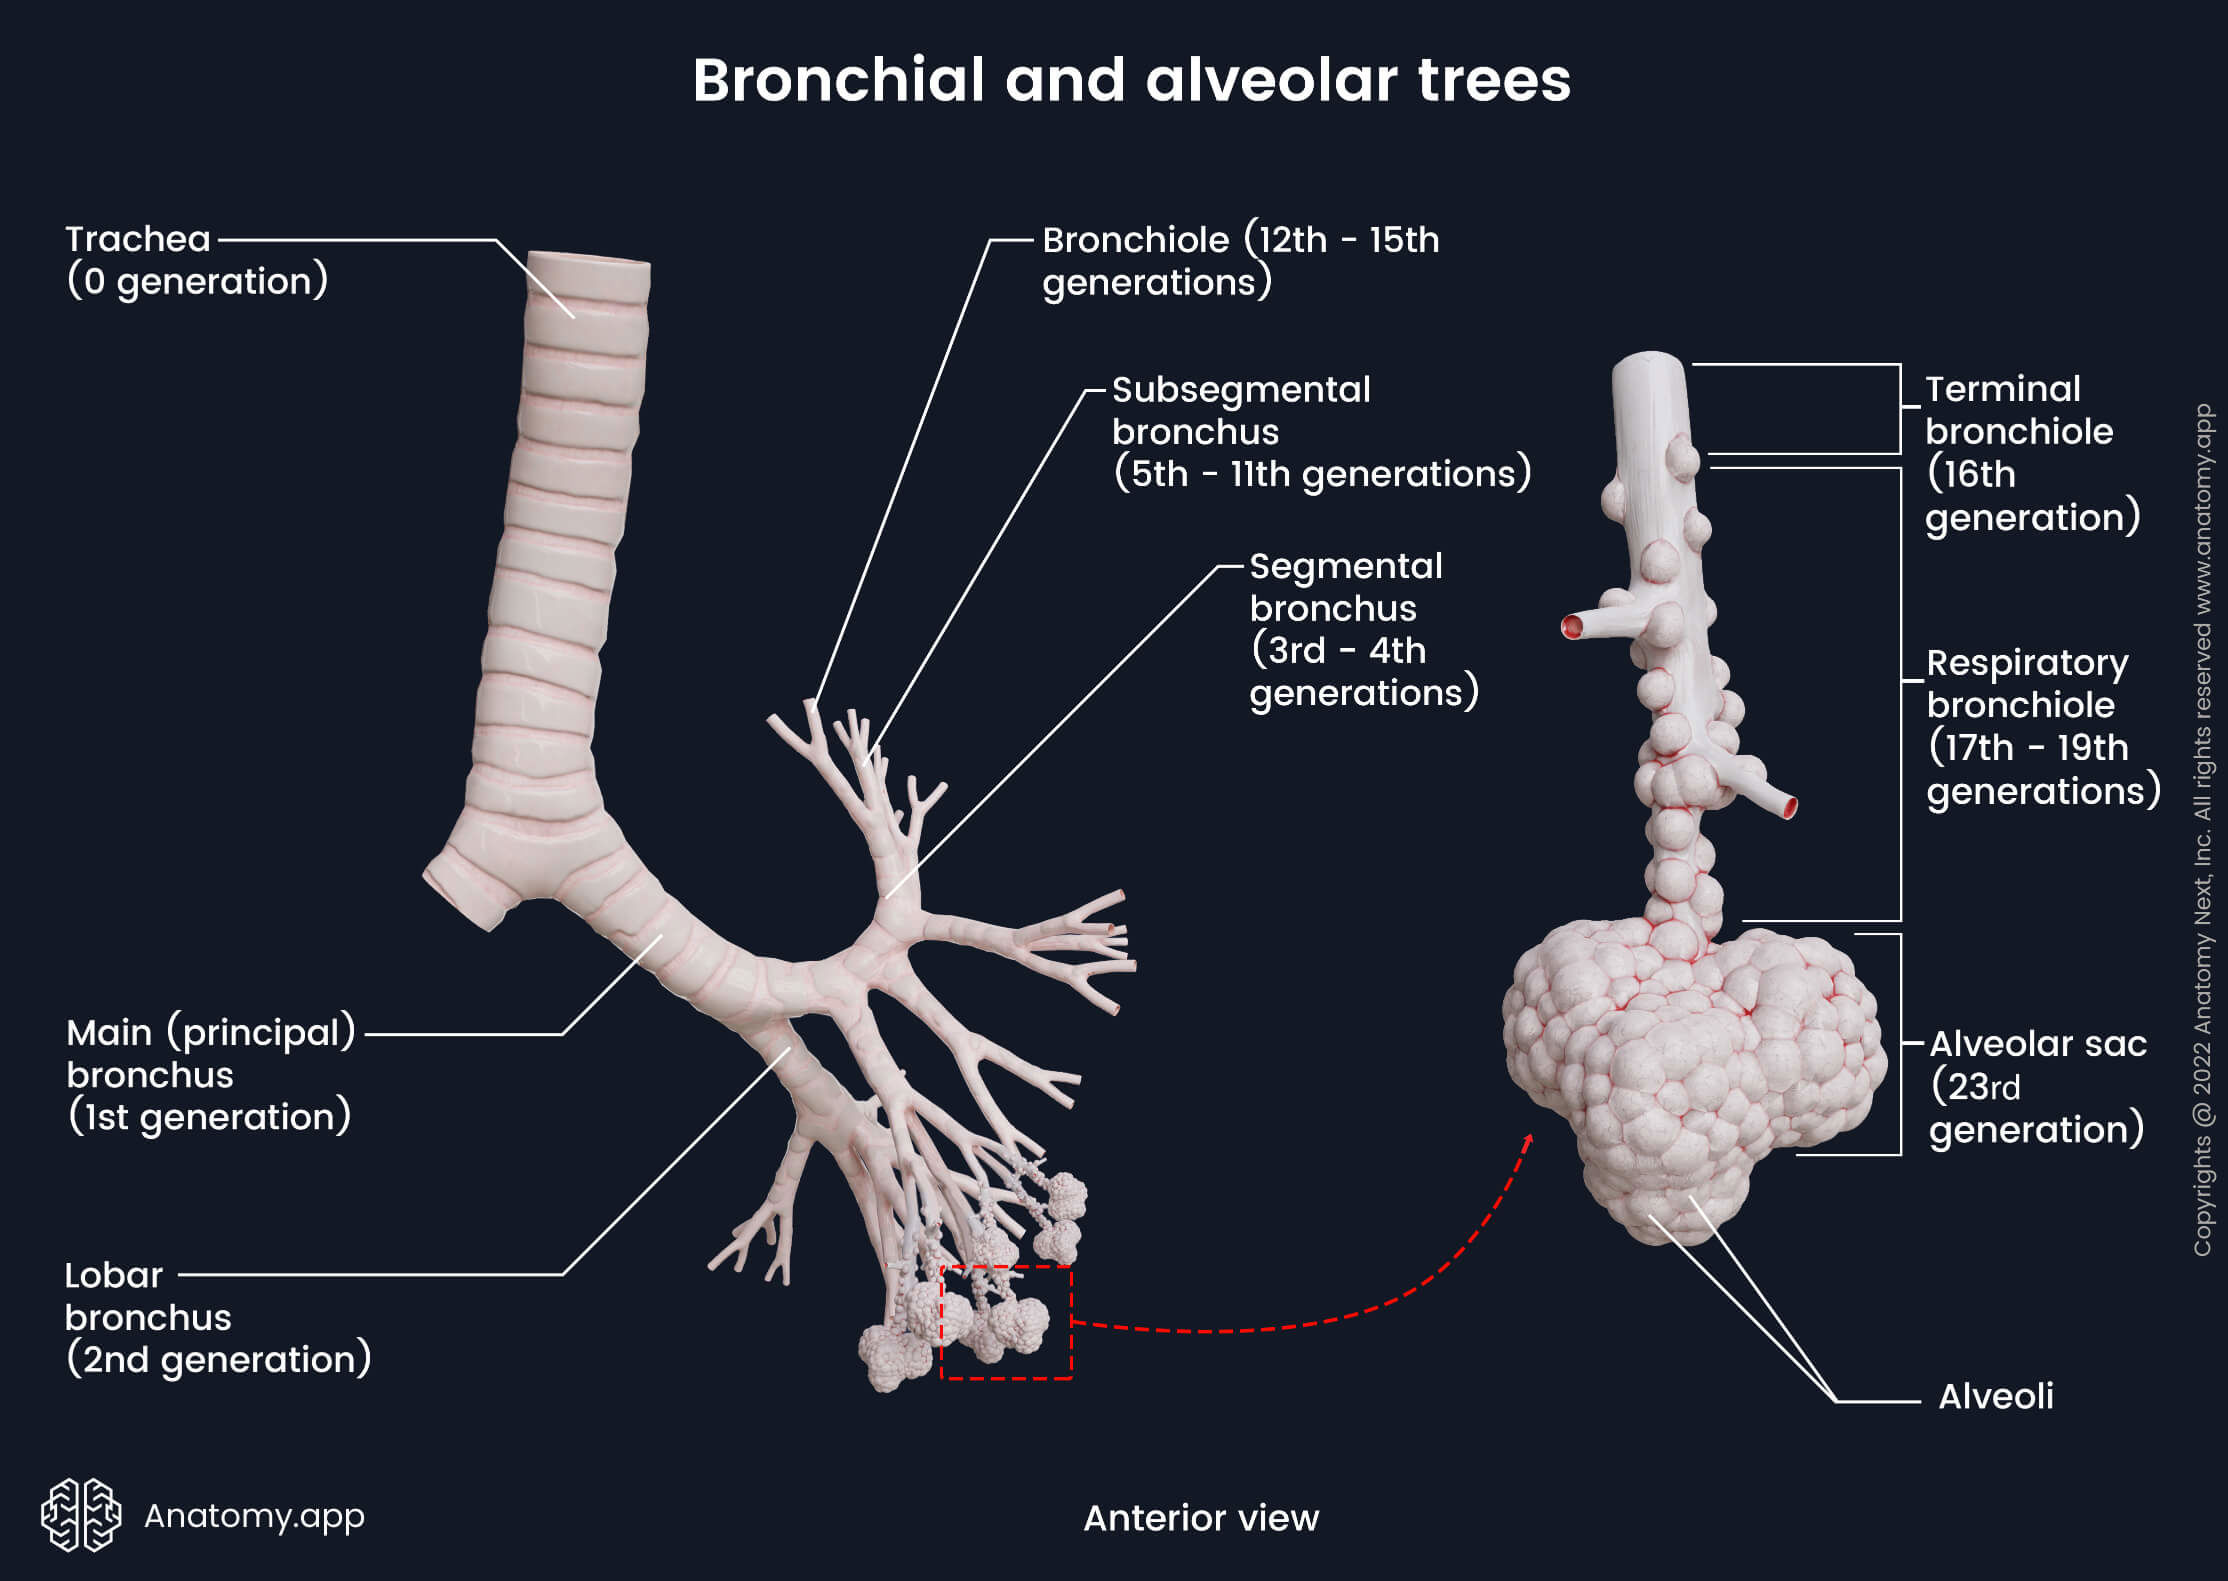
\includegraphics[width=\textwidth]{figures/airway_bronchial_alveolar_trees.jpg}  % user-supplied image, unmodified
  \caption{Bronchial and alveolar trees (anterior view). The conducting airways run from the
           trachea (generation 0) through the main, lobar, segmental and subsegmental bronchi and
           the bronchioles to the terminal bronchioles (generation 16); the enlarged detail shows
           the respiratory zone, with respiratory bronchioles (generations 17--19) and an
           alveolar sac (generation 23) covered with alveoli. The generation ranges differ
           slightly between sources (compare Table~\ref{tab:weibel_generations}). Image
           \copyright~2022 Anatomy Next, Inc., reproduced from Anatomy.app \cite{anatomyapp}.}
  \label{fig:anatomy_overview}           % referenced as Figure~\ref{fig:anatomy_overview}
\end{figure}

\paragraph{Structure and function.}      % conducting vs respiratory zone, generations
Starting from the trachea, each airway divides into daughter branches of smaller diameter and
length. The branching level is counted in \emph{generations}: in the classical symmetric model
of \citet{weibel1963}, the trachea is generation~0 and every airway splits into two, so that
generation $z$ contains $2^z$ airways and the tree ends after 23 generations
(Table~\ref{tab:weibel_generations}). Generations 0 to 16 form the \emph{conducting zone}:
the trachea, bronchi and bronchioles down to the terminal bronchioles. They take no part in gas
exchange; they conduct, warm, humidify and filter the inspired air, and their volume forms the
anatomical dead space. Generations 17 to 23 form the \emph{respiratory zone}, whose
respiratory bronchioles, alveolar ducts and alveolar sacs carry the alveoli in which oxygen and
carbon dioxide diffuse between air and blood \cite{weibel1963}. Because the number of airways
doubles at each generation while their diameter shrinks by only about a fifth, the total
cross-section grows quickly towards the periphery and the air slows down, so that transport in
the deepest generations is dominated by diffusion. The bronchi are supported by cartilage,
whereas the bronchioles are not; the non-cartilaginous airways with an internal diameter below
about 2~mm, found from roughly the eighth generation onwards, are called the \emph{small
airways} \cite{burgel2013small}. Real airway trees are not symmetric: the two daughters of a
bifurcation usually differ in diameter, length and angle, and the number of generations
between the trachea and a terminal bronchiole varies from one path to another
\cite{horsfield1971models,kitaoka1999}.

\begin{table}[htbp]                      % Weibel's symmetric model, grouped by zone
  \centering                             % center the table
  \small                                 % slightly smaller font so the table fits
  \caption{Airway generations in the symmetric model of \citet{weibel1963}. Diameters are
           approximate model values for an adult lung; real trees are asymmetric, so the
           correspondence between generation and airway type is only indicative. The last
           column indicates which airways clinical CT can resolve
           \cite{burgel2013small}.}
  \label{tab:weibel_generations}         % referenced as Table~\ref{tab:weibel_generations}
  \begin{tabular}{llccc}                 % zone, airway, generation, diameter, CT
    \toprule
    Zone & Airway & Generation $z$ & Diameter (mm) & Clinical CT \\
    \midrule
    Conducting  & Trachea                & 0       & 18        & Yes \\
                & Main bronchi           & 1       & 12        & Yes \\
                & Lobar bronchi          & 2       & 8         & Yes \\
                & Segmental bronchi      & 3       & 6         & Yes \\
                & Subsegmental bronchi   & 4       & 4.5       & Yes \\
                & Small bronchi          & 5--11   & 3.5--1.1  & Partly \\
                & Bronchioles            & 12--15  & 1.0--0.7  & No \\
                & Terminal bronchioles   & 16      & 0.6       & No \\
    \midrule
    Respiratory & Respiratory bronchioles & 17--19 & 0.5       & No \\
                & Alveolar ducts         & 20--22  & 0.4       & No \\
                & Alveolar sacs          & 23      & 0.4       & No \\
    \bottomrule
  \end{tabular}
\end{table}

\paragraph{Anatomical nomenclature.}     % lobes and segments (Table)
Below the generation count, airways are named after the lung region they supply. At the carina
the trachea divides into the right and left main bronchi. The right lung has three lobes
(upper, middle and lower) and the left lung two (upper, including the lingula, and lower), each
supplied by a lobar bronchus. The lobar bronchi divide into \emph{segmental bronchi}, each
ventilating one bronchopulmonary segment. The right lung has ten segmental bronchi, RB1 to
RB10; in the left lung, the apical and posterior segments and the anterior and medial basal
segments usually share a bronchus (LB1+2 and LB7+8), which gives eight segmental bronchi
(Table~\ref{tab:segmental_bronchi}). This nomenclature goes back to systematic studies of the
bronchopulmonary segments \cite{boyden1949}, which also documented how frequent anatomical
variations are, for example trifurcations of the right upper lobe bronchus in almost half of
the subjects \cite{boyden1949} and of the left upper division and lower lobar bronchi in about
a fifth \cite{zhao2009}. The $10+8=18$ segmental bronchi, together with the trachea and main
bronchi, are the classes predicted by the labelling model used in this work
(\secref{sec:labeling}) \cite{xie2025}.

\begin{table}[htbp]                      % segmental bronchi per lobe
  \centering                             % center the table
  \small                                 % slightly smaller font so the table fits
  \caption{Lobar and segmental bronchi of the human airway tree.}
  \label{tab:segmental_bronchi}          % referenced as Table~\ref{tab:segmental_bronchi}
  \begin{tabular}{lll}                   % lung, lobe, segmental bronchi
    \toprule
    Lung  & Lobe   & Segmental bronchi \\
    \midrule
    Right & Upper  & RB1 apical, RB2 posterior, RB3 anterior \\
          & Middle & RB4 lateral, RB5 medial \\
          & Lower  & RB6 superior, RB7 medial basal, RB8 anterior basal, \\
          &        & RB9 lateral basal, RB10 posterior basal \\
    \midrule
    Left  & Upper  & LB1+2 apicoposterior, LB3 anterior, \\
          &        & LB4 superior lingular, LB5 inferior lingular \\
          & Lower  & LB6 superior, LB7+8 anteromedial basal, \\
          &        & LB9 lateral basal, LB10 posterior basal \\
    \bottomrule
  \end{tabular}
\end{table}

\paragraph{What current imaging can resolve.}  % CT resolution limits
Clinical CT has a spatial resolution of about 0.6 to 1~mm, which allows direct assessment of
airways down to a diameter of about 2 to 2.5~mm; normal bronchioles are not visible
\cite{burgel2013small}. The datasets used in this work fall in this range, with in-plane
resolutions of 0.5 to 0.92~mm and slice thicknesses of 0.45 to 1~mm for ATM'22
(\secref{sec:atm22}). In Weibel's model, the airway diameter falls below 2~mm around the eighth
generation (Table~\ref{tab:weibel_generations}); in real, asymmetric trees this happens
earlier along many paths, and in patients with COPD most sixth-generation airways of the
apical and posterior basal segments are already narrower than 2~mm \cite{tanabe2019peripheral}.
A lumen that spans only one or two voxels is also blurred by the partial volume effect, so
segmentations lose branches and suffer breakages towards the periphery \cite{zhang2024}.
Ultra-high-resolution CT, with 0.25~mm slices and $1024 \times 1024$ matrices, can measure
airways of 1 to 2~mm in vivo \cite{tanabe2018uhrct,tanabe2019peripheral}, and smaller airways
have so far been studied mainly with histology and micro-CT on excised lungs
\cite{tanabe2018uhrct}. MRI, with hyperpolarized gases or ultrashort echo times, avoids
ionizing radiation but has a lower resolution and reaches at most the segmental and
subsegmental bronchi \cite{lewis2005,genkin2024}. In practice, an airway tree segmented from CT
therefore contains the central airways and a limited number of further generations, only a
small fraction of the tens of thousands of terminal bronchioles of the real tree.

\paragraph{Estimating the complete tree.}  % models beyond CT resolution
Because the peripheral airways cannot be imaged in vivo, the complete tree is estimated with
models. Anatomically based models grow the tree inside the lung volume with fractal-like or
volume-filling rules that reproduce morphometric data \cite{kitaoka1999,tawhai2000}
(Figure~\ref{fig:anatomy_fractal}). Patient-specific models combine both: the lobes and the
central airways are segmented from CT, and the tree beyond CT resolution is generated inside
each lobe, guided by the resolved airways and the lobar boundaries
\cite{tawhai2004,bordas2015,pennati2024modeling} (Figure~\ref{fig:anatomy_pipeline}). AVATREE
follows the same idea and can extend a CT-derived tree to any number of generations
\cite{nousias2020avatree} (Figure~\ref{fig:anatomy_generations}). The comparison between the
central airways and the estimated tree in these figures shows how small the CT-visible part of
the airway tree is. All the airway trees used in this work, and therefore all the
representations and models of the following sections, are limited to this CT-resolved part.

\begin{figure}[htbp]                     % fractal-like 3D model of the complete tree
  \centering                             % center the figure
  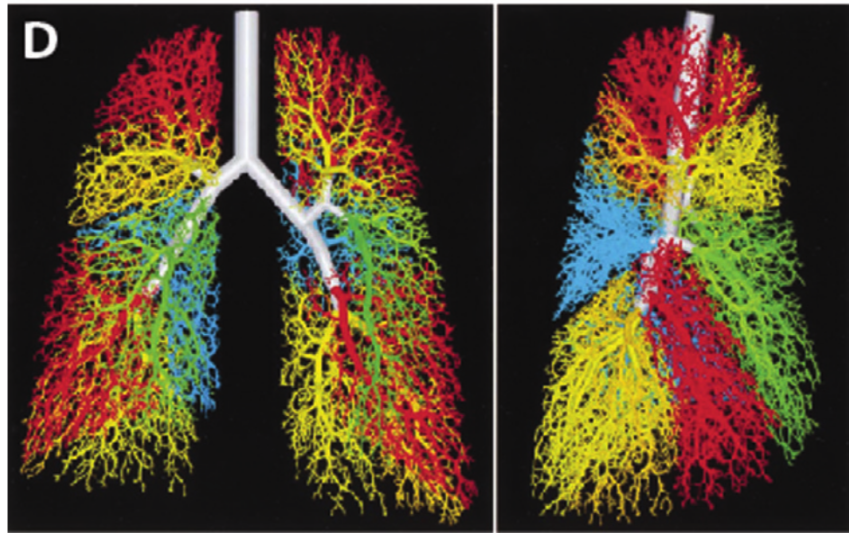
\includegraphics[width=0.75\textwidth]{figures/airway_fractal_model.png}  % front and side views
  \caption{Three-dimensional model of the human airway tree generated with fractal-like rules,
           in front and side views. The model contains more than 50,000 branches and matches
           morphometric data from human lungs. Reproduced from
           \citet{varner2017computational}, who adapted it from earlier work.}
  \label{fig:anatomy_fractal}            % referenced as Figure~\ref{fig:anatomy_fractal}
\end{figure}

\begin{figure}[htbp]                     % CT -> segmentation -> complete tree
  \centering                             % center the figure
  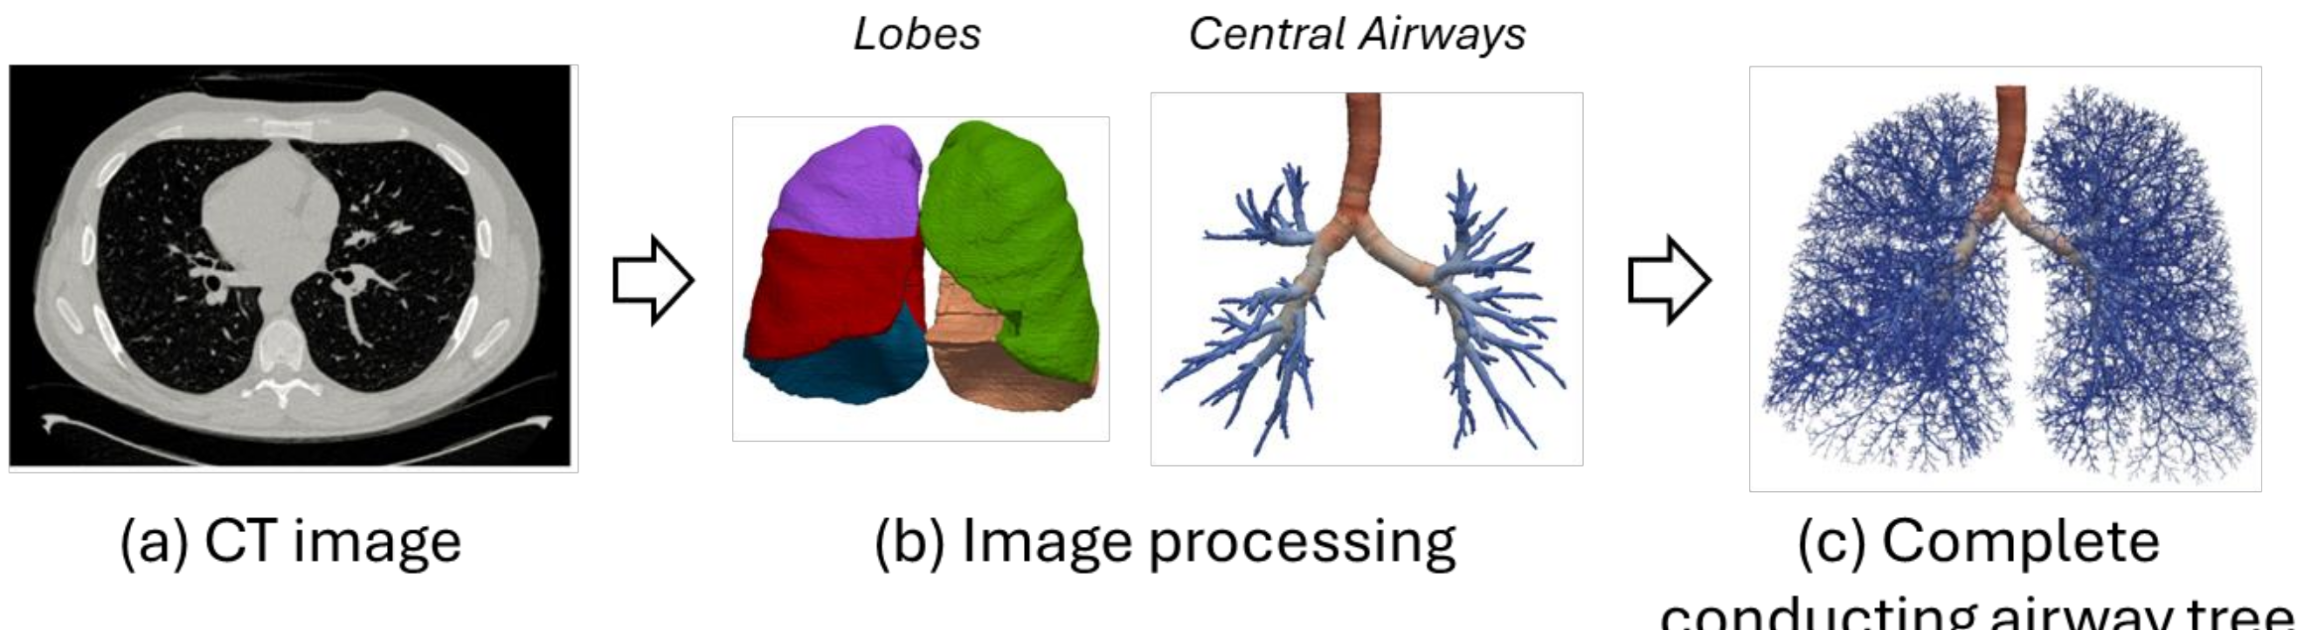
\includegraphics[width=\textwidth]{figures/airway_ct_to_complete_tree.png}  % three-step pipeline
  \caption{Patient-based model of the complete conducting airway tree: (a) CT image; (b) lobes
           and central airways segmented from the CT image; (c) airway tree beyond CT
           resolution generated with a lobe-filling algorithm, colour-coded by airway radius.
           Reproduced from \citet{pennati2024modeling}, who adapted it from earlier work.}
  \label{fig:anatomy_pipeline}           % referenced as Figure~\ref{fig:anatomy_pipeline}
\end{figure}

\begin{figure}[htbp]                     % 12 vs 23 estimated generations
  \centering                             % center the figure
  \begin{minipage}[b]{0.49\textwidth}    % left panel
    \centering                           % center inside the panel
    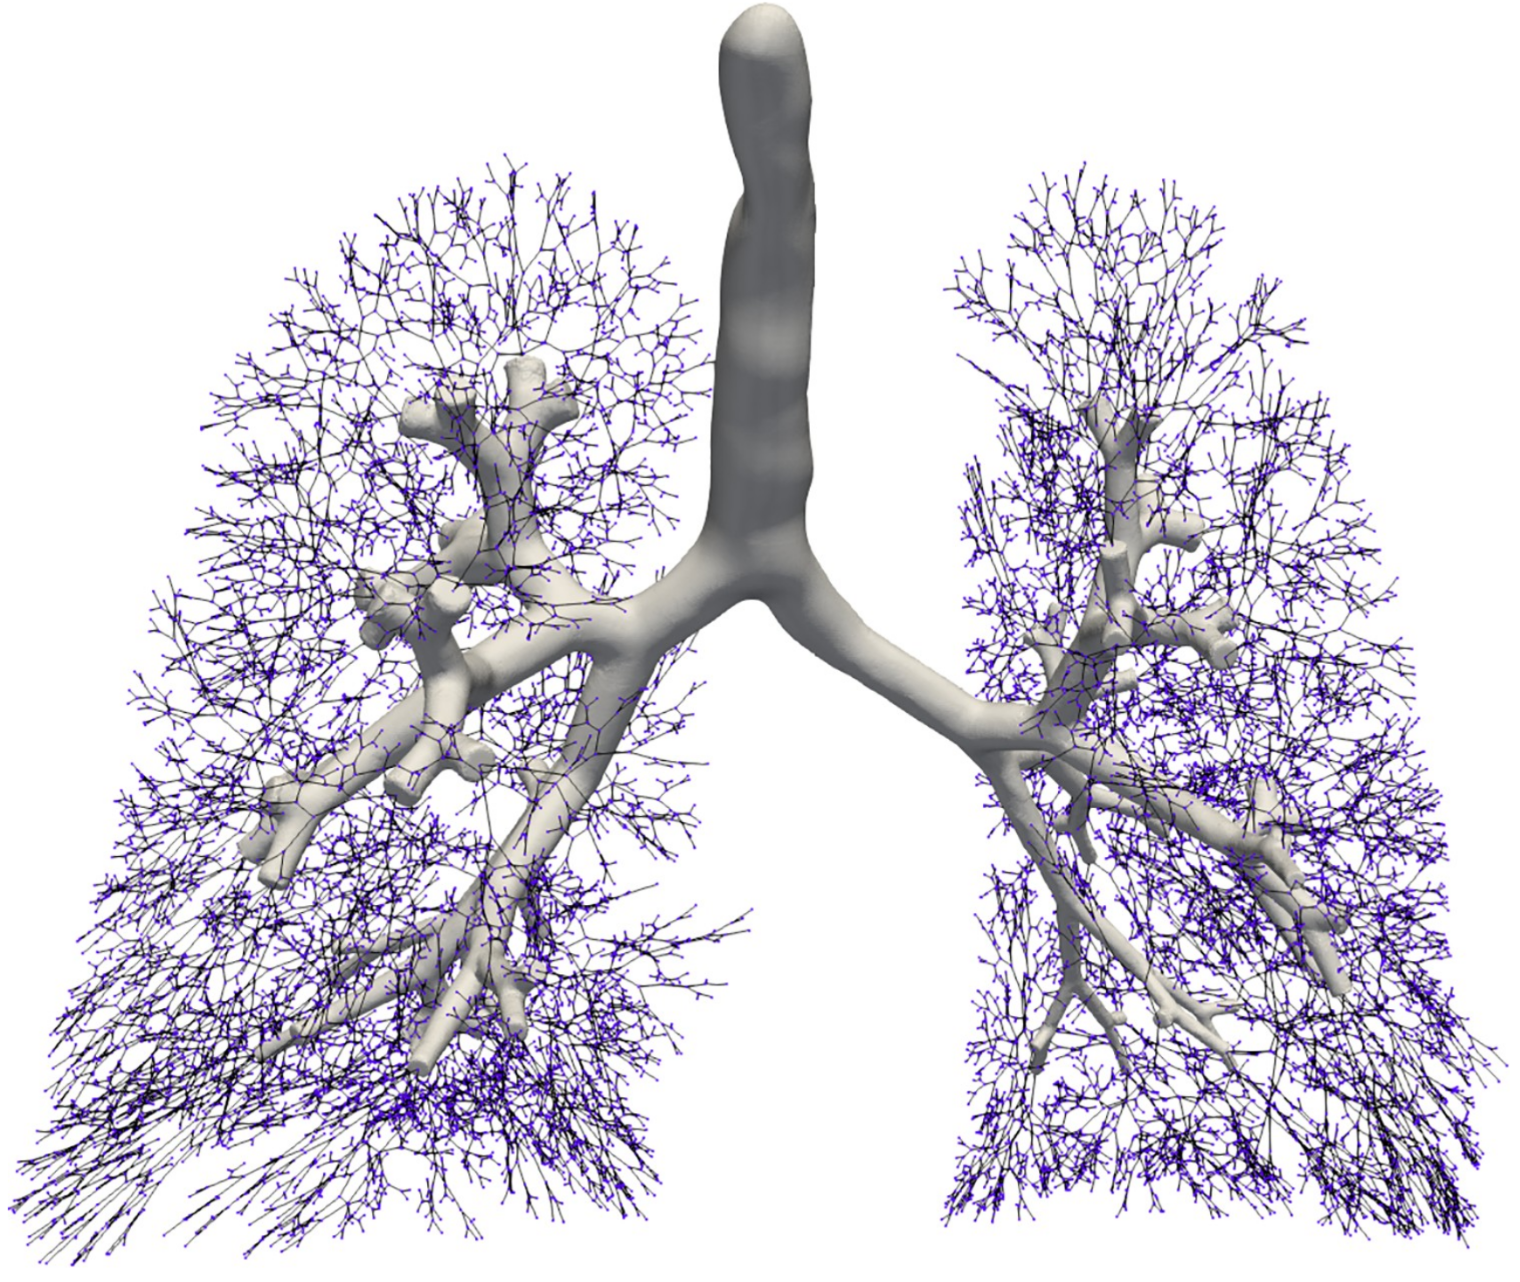
\includegraphics[width=\textwidth]{figures/airway_estimated_12gen.png}  % 12 generations
    \par\small (a) 12 generations        % panel label
  \end{minipage}\hfill                   % space between the panels
  \begin{minipage}[b]{0.49\textwidth}    % right panel
    \centering                           % center inside the panel
    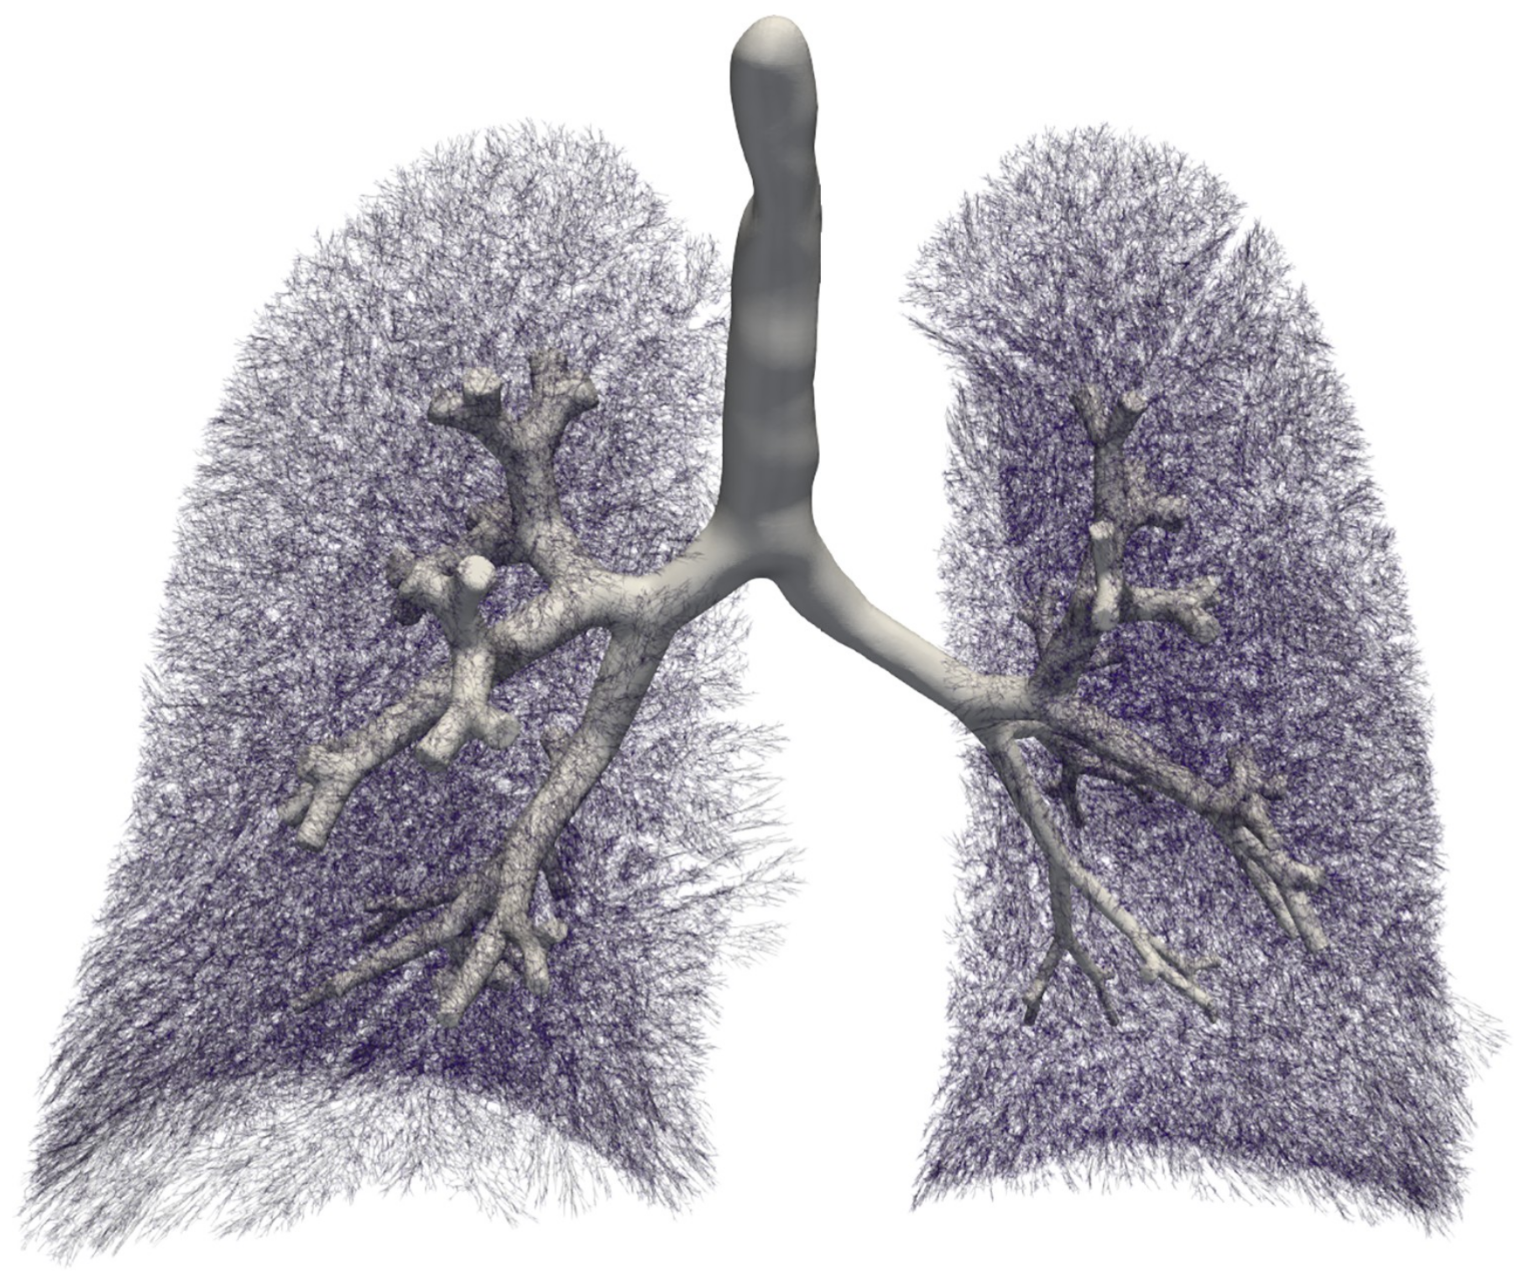
\includegraphics[width=\textwidth]{figures/airway_estimated_23gen.png}  % 23 generations
    \par\small (b) 23 generations        % panel label
  \end{minipage}
  \caption{Bronchial tree estimated from a CT-derived airway tree up to (a) 12 and (b) 23
           generations. The surface is reconstructed for the first 7 generations; deeper
           generations are shown as centerlines. Reproduced from
           \citet{nousias2020avatree}.}
  \label{fig:anatomy_generations}        % referenced as Figure~\ref{fig:anatomy_generations}
\end{figure}
              % Subsection "Anatomy of the pulmonary airways"
% Data representation -- the ways a 3D airway tree can be stored, and where each is used here.
% Subsection of "Background", pulled in by sections/02-background.tex.
% The figure is generated by figures/make_airway_representations.py (synthetic tree).

\subsection{Data representation}         % how a 3D airway tree can be stored
\label{sec:data_representation}          % \secref{sec:data_representation}

A 3D pulmonary airway tree can be stored in several ways. The choice matters as it fixes what a
model sees (a volume, a surface, sample points or a skeleton), how much memory it needs, and
whether the branching structure is explicit or has to be inferred.
Figure~\ref{fig:airway_representations} shows the same tree in six common
representations, and Table~\ref{tab:airway_representations} summarizes their main properties.

\begin{figure}[htbp]                     % the six representations on one synthetic tree
  \centering                             % center the figure
  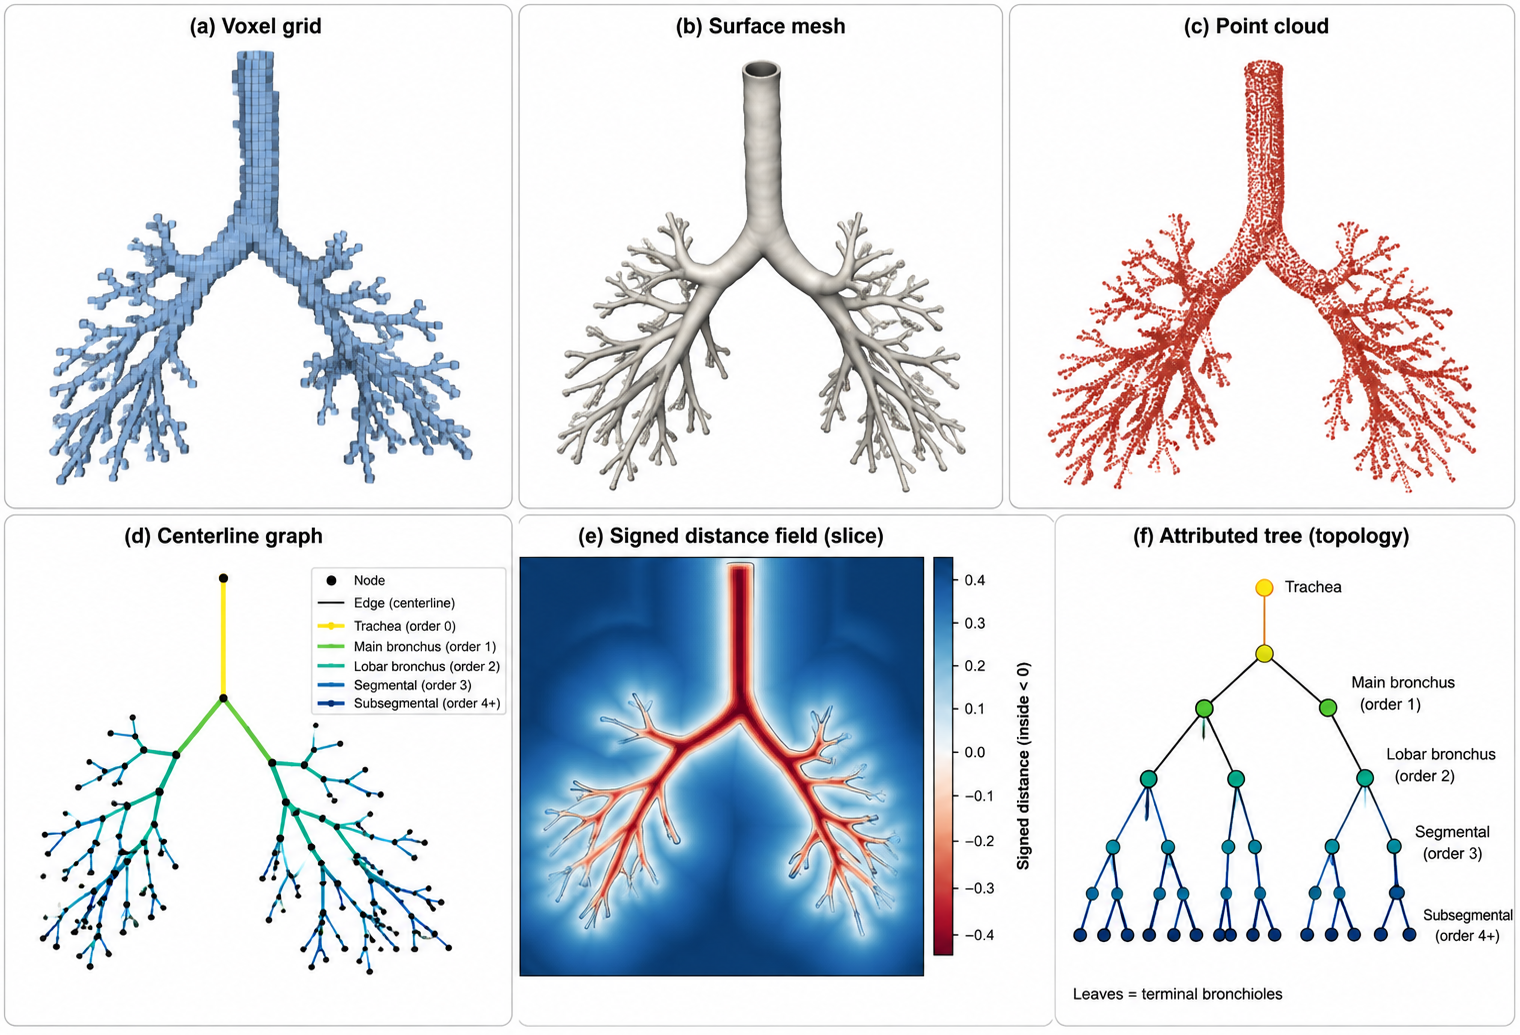
\includegraphics[width=\textwidth]{figures/airway_representations.png}  % made by figures/make_airway_representations.py
  \caption{The same synthetic airway tree (trachea and three generations) in six
           representations: (a) binary voxel grid, (b) triangulated surface mesh, (c) point
           cloud sampled on the surface, (d) centerline graph, with edge colour and width
           following the branch radius, (e) signed distance field on a slice through the first
           bifurcation, with the airway surface as the zero level set (black line), and
           (f) the abstract tree topology, whose edges carry attributes such as radius $r$ and
           length $\ell$.}
  \label{fig:airway_representations}     % referenced as Figure~\ref{fig:airway_representations}
\end{figure}

\paragraph{Voxel grid.}                  % (a) binary occupancy on a regular grid
The airway is a binary occupancy mask on a regular 3D grid, usually the grid of the CT scan
itself. This is the direct output of manual annotation and of segmentation networks, and the
format in which ATM'22 and AIIB23 are distributed (\secref{sec:datasets}). It fits 3D
convolutional networks naturally \cite{brock2016,garciauceda2021}, but memory grows with the
cube of the resolution while almost all voxels are empty, and the shape is limited by the voxel
spacing: thin distal branches cover only a few voxels and tend to look jagged or broken
\cite{zhang2024}. Sparse variants store only the occupied voxels, for example with the VDB
data structure \cite{museth2013} used by XCube \cite{ren2024}, or with sparse convolutions
\cite{prabhakar2026vaesselsparse}. In this work, voxel grids are used for registration
and by the dense and sparse autoencoders.

\paragraph{Surface mesh.}                % (b) triangulated lumen boundary
A surface mesh describes the boundary of the airway lumen with vertices and triangles. It is
usually extracted from the voxel mask with Marching Cubes \cite{lorensen1987}, or
reconstructed from points, e.g.\ by Poisson surface reconstruction in AVATREE
\cite{nousias2020avatree}. Meshes are compact, give sub-voxel smooth surfaces and are the
standard input for flow simulation \cite{lauria2022,ho2024}, but they carry no explicit branch
structure and can contain non-manifold elements, which is why their number is used as a
quality metric \cite{zhang2024}. In this work, meshes are extracted as the first step of the
implicit model's data preparation.

\paragraph{Point cloud.}                 % (c) unordered sample points
A point cloud is an unordered set of 3D points sampled on the surface of the airway tree. It
is sparse and independent of any grid, and it can be processed by point networks such as
PointNet++ \cite{qi2017} and Point Transformer \cite{zhao2021}. It has no connectivity, however,
so thin branches may receive too few points to be recognized. 
% In this work, IPGN samples
% foreground voxels as a point cloud, and the implicit model is trained on
% points sampled on and around the surface.

\paragraph{Centerline graph.}            % (d) skeleton as nodes and edges
Thinning the binary mask gives a one-voxel-wide skeleton \cite{lee1994,palagyi2006}, which can
be converted into a graph whose nodes are bifurcations and end points and whose edges are the
branches between them \cite{bumgarner2022}. Each edge can carry attributes such as radius,
length and direction. The representation is very compact and makes the branching topology
explicit, which is why it underlies most work on branch labeling
\cite{tschirren2005matching,feragen2011airway,xie2025}, morphometry
\cite{kaji2024airway,zhang2025airmorph} and graph generation \cite{prabhakar2024vesselgraph}.
Its weaknesses are its sensitivity to skeletonization artefacts, such as spurious short branches,
and the loss of the lumen shape beyond the stored attributes. In this work, the centerline
graph is an input of IPGN - the model that used to generate the labels - and the basis of the morphological
descriptors.

\paragraph{Implicit function.}           % (e) zero level set of a continuous field
The surface can also be defined as the zero level set of a continuous function of space,
typically a signed distance field (SDF) that is negative inside the airway and positive
outside. Neural implicit representations learn this function with a small network conditioned
on a latent code \cite{park2019,sitzmann2020}, or store it in feature planes that can be queried
anywhere \cite{weng2026topofield}. The result is continuous, resolution-free and smooth, but a
mesh has to be extracted to visualize it, and the topology is not explicit; DGCI addresses this
by learning correspondences through a space shared by all trees \cite{zhang2024}. In this work,
the implicit representation is the one that produced the best reconstructions.

\paragraph{Attributed tree and parametric models.}  % (f) abstract topology with attributes
Finally, the airway can be reduced to a combinatorial tree whose edges carry geometric
attributes, such as radius, length or landmark points along the branch. Idealized airway
models describe the whole tree this way \cite{horsfield1971models,kitaoka1999}, tree-shape
spaces use it to compare and average trees \cite{feragen2011means,feragen2011airway}, and
generative models encode it recursively \cite{feldman2023vesselvae,batten2025vetta} or as a
sequence of nodes \cite{feldman2025vesselgpt}. Branch geometry can in turn be described
parametrically, e.g.\ with NURBS \cite{ortizpuerta2022} or B-spline cross-sections
\cite{feldman2025vesselgpt}. Such representations are compact and interpretable, but they
depend on a reliable extraction of the tree, and trifurcations or loops break the assumption of
a binary tree \cite{miyawaki2017automatic}. The morphological descriptors used in this work
operate on such a tree, whose nodes carry an anatomical label, a generation number and a length.

\begin{table}[htbp]                      % side-by-side comparison of the representations
  \centering                             % center the table
  \small                                 % slightly smaller font so the table fits
  \caption{Main properties of the airway tree representations, and where each one is used in
           this work.}
  \label{tab:airway_representations}     % referenced as Table~\ref{tab:airway_representations}
  \begin{tabular}{llcl}                  % name, geometry, explicit branching, use here
    \toprule
    Representation   & Geometry            & Branching explicit & Used in this work \\
    \midrule
    Voxel grid       & Discrete volume     & No  & Registration, VAE, autoencoders \\
    Sparse voxels    & Occupied voxels     & No  & Sparse encoder \\
    Surface mesh     & Continuous surface  & No  & Implicit model (data preparation) \\
    Point cloud      & Sampled points      & No  & Labelling (IPGN), Implicit model \\
    Centerline graph & 1D skeleton         & Yes & Labelling (IPGN), morphological metrics \\
    Implicit (SDF)   & Continuous field    & No  & Implicit encoding (DGCI) \\
    Attributed tree  & Abstract topology   & Yes & Morphological metrics \\
    \bottomrule
  \end{tabular}
\end{table}
  % Subsection "Data representation"
% Related work -- prior work grouped by scope, roughly oldest first within each group.
% Subsection of "Background", pulled in by sections/02-background.tex.

\subsection{Related work}                % prior work on airway geometry, segmentation, CFD, encoding, labelling, morphology
\label{sec:related}                      % \secref{sec:related}

% ==============================================================================
\subsubsection{Geometric models of the airway tree}  % morphometry, generation, casts, CT-based and hybrid models
\label{sec:related_geometry}             % \secref{sec:related_geometry}

\paragraph{Morphometry and idealized models.}  % from lung casts to mathematical descriptions
Early airway models are based on idealized morphometry rather than on individual anatomy.
Casts of human lungs were used to study branching patterns and the relation between airway
lengths and diameters \cite{horsfield1986}, and \citet{horsfield1971models} and
\citet{yeh1980models} proposed asymmetric models of the human bronchial tree.
\citet{kamiya1974} related airway diameter to branching angles, and \citet{wang1992} examined
deterministic bifurcating distributive systems with a Monte Carlo method.
\citet{kitaoka1999} proposed a 3D model of the human airway tree in which the branching
pattern is driven by a diameter--flow relationship within an organ boundary, relating
branching angle to flow rate and airway length to diameter. \citet{hegedus2004} gave a
detailed mathematical description of airway bifurcation geometry and used it to generate
surface models of idealized bifurcations, and \citet{florens2010} presented an anatomical and
functional model of the tracheobronchial tree. \citet{tawhai2011} reviewed computational
models of airway and pulmonary vascular structure and function towards a ``Lung Physiome''.

% \citet{varner2017computational} reviewed computational approaches to airway branching
% morphogenesis in the mammalian lung, grouping them into three classes: geometric,
% reaction--diffusion, and continuum mechanical models. Geometric models, inspired by
% Mandelbrot's fractal theory, show that simple recursive rules can generate space-filling,
% lung-like trees that match morphometric data, but they do not explain the biological
% mechanisms behind these rules. Physical models, including viscous fingering, buckling driven
% by constrained epithelial growth, and apical constriction, show that mechanical forces can
% also determine where branches form. The authors argue that each framework captures only part
% of the process, and that future models should combine biochemical and mechanical cues and be
% grounded in quantitative experimental data from embryonic lungs.

\paragraph{Algorithmic generation of airway trees.}  % volume filling and L-systems
Building on the Monte Carlo approach of \citet{wang1992}, \citet{tawhai2000} introduced a
volume-filling algorithm that grows a bifurcating tree inside each lung lobe.
\citet{davoodi2016} generated the human bronchial tree with a Lindenmayer system, and
\citet{abbasi2021} extended it to a stochastic parametric L-system with parallel growth of
bronchopulmonary segments. \citet{geronzi2024} proposed a parametric 3D model of human
airways for particle drug delivery and deposition.

% \paragraph{Lung casts and digital reference models.}  % physical replicas
% \citet{clinkenbeard2002} built hollow airway replicas of the first five generations using
% rapid prototyping. \citet{schmidt2004} created a digital reference model of the bronchial tree
% (17 generations) by segmenting a CT scan of a rubber lung cast, and \citet{lizal2012} derived
% realistic and semi-realistic airway geometries up to the seventh bifurcation from it.

\paragraph{Subject-specific models from CT.}  % CT-resolved airways, often extended algorithmically
Subject-specific airway trees can be extracted from CT images. \citet{palagyi2006} developed
the skeletonization used to obtain a 1D tree from a segmented airway, and
\citet{nakamura2008} presented automated segmentation and morphometric analysis of the airway
tree from multidetector CT. \citet{tawhai2004} combined CT-based geometry analysis with finite
element models of the human and ovine bronchial tree, using their volume-filling algorithm to
extend the CT-resolved tree to the terminal bronchioles, guided by the resolved airways and
the lobar boundaries. \citet{lin2009} and \citet{tawhai2009} combined CT-based central airways
with such artificial airways to build subject-specific models from the glottis to the
terminal bronchioles for CFD, but their pipeline required manual intervention to construct
trifurcations; \citet{lin2013} later reviewed multiscale image-based modeling of gas flow and
particle transport in the lungs. \citet{montesantos2013} reported HRCT-based airway
morphometry in healthy subjects and asthmatic patients, and \citet{montesantos2016} presented
an algorithm for an individualized 3D deterministic model of the human bronchial tree from
HRCT images, which they evaluated statistically. \citet{bordas2015} developed a pipeline for
patient-based complete conducting airway models of healthy and asthmatic subjects, covering
CT acquisition, lung, lobar and airway segmentation, centerline extraction, and algorithmic
generation of the distal airways beyond the CT-resolved tree.

Trifurcations are a frequent source of difficulty for these models, although they are common
in real airway trees. \citet{boyden1949} studied bronchopulmonary segments in 50 subjects and
reported a trifurcation at the right upper lobe bronchus in 46\% of them, and
\citet{zhao2009} examined the left-lung bronchial anatomy of 216 subjects with multi-detector
CT and found trifurcations at the left upper division bronchus and the left lower lobar
bronchus in 23\% and 18\% of subjects, respectively.

\citet{miyawaki2017automatic} proposed a centerline-based method that automatically
constructs subject-specific three-dimensional models of the human airways from a CT-segmented
airway skeleton and surface. Their approach systematically identifies and classifies
trifurcations, distinguishing true trifurcations from double bifurcations and fork-type from
tripod-type configurations, and uses dedicated geometric templates to reconstruct them. The
method produces models of increasing realism (straight-centerline, curved-centerline, and
fitted-surface), can be extended beyond CT resolution to the terminal bronchioles, and
partitions the geometry branch by branch, which facilitates automatic mesh generation for
computational fluid dynamics (CFD). Applied to 16 healthy and 16 severe asthmatic subjects,
the fitted-surface models achieved an average surface error of about 11\% of the image voxel
size, and an aerosol deposition simulation showed branch-wise deposition efficiencies within
5\% of those obtained with a CT-based model.

\citet{nousias2020avatree} presented AVATREE for generating
anatomically valid patient-specific airway tree models from CT scans. Their pipeline first
segments the lungs and the visible central airways and extracts the airway centerline as a
graph. It then extends the tree beyond the generations visible in the image using a
space-filling algorithm which splits the lung volume with PCA based planes. From the extended
centerline they reconstruct a 3D airway surface suitable for CFD simulations using Poisson
surface reconstruction. The framework also produces spatial probability maps of airway
generations overlaid on the CT images. It can simulate broncho-constriction as seen in asthma
and COPD, through Laplacian mesh contraction. The authors validated the generated trees
against published morphometric data comparing Strahler and Horsfield orders, branch lengths,
diameters and branching angles.

\paragraph{Meshing and hybrid models.}   % from segmented geometry to simulation-ready meshes
\citet{marchandise2013} proposed an automatic method to build and mesh tubular geometries,
including trifurcations, for cardiovascular and lung applications. However, it takes a surface
as input and is not centerline based, so the mesh patches are not linked to branches with
anatomical data. \citet{lauria2022} developed an automatic method to generate CFD compliant
triangulated meshes from segmented airways, \citet{ortizpuerta2022} introduced Snakes
Isogeometric Analysis based on NURBS for healthy and COPD airway trees and \citet{ho2024}
smoothed airway surface meshes with graph convolutional neural networks. Following the same
idea as \citet{bordas2015}, \citet{agujetas2020} and \citet{ilegbusi2023} built hybrid models
that couple image derived upper airways with idealized lower airways for CFD.

\citet{pennati2024modeling} presented a comprehensive review of geometrical models of the
human intrathoracic airways tracing their evolution from the early idealized mathematical
models of the 1960s such as the symmetric Weibel model and the asymmetric Horsfield model,
to modern image-based, patient-specific reconstructions derived from CT and to a lesser
extent. The authors surveyed airway segmentation strategies ranging from traditional
region-growing and knowledge-based methods to machine learning and deep learning approaches
such as 3D U-Net architectures and outlined the pipeline required to obtain CFD compliant
meshes including centerline extraction, surface smoothing and mesh generation. They also
discussed hybrid models that combine CT-resolved central airways with algorithmically
generated distal trees and reviewed applications in inter-subject variability studies,
diagnosis, surgical planning, drug delivery and environmental exposure. Finally, they
identified key open challenges including missing small airways in segmentation, limited
validation on pathological scans and the need for robust, automated mesh generation suitable
for clinical use.

% % ==============================================================================
% \subsubsection{Airway segmentation and benchmarks}  % extracting the tree from CT and MRI
% \label{sec:related_segmentation}         % \secref{sec:related_segmentation}

% \paragraph{Traditional methods.}         % region growing, rules, morphology, tubes
% Early methods segmented the airway tree from CT by region growing \cite{mori1995}, later
% combined with rule-based and knowledge-based strategies exploiting the relation between
% airways and vessels \cite{sonka1996}, fuzzy logic \cite{park1998}, mathematical morphology
% and topology \cite{pisupati1996,fan2000}, tube detection \cite{bauer2009tube} and gradient
% vector flow \cite{bauer2009gvf}. \citet{lo2009} extracted airway trees via locally optimal
% paths, and \citet{irving2011} segmented obstructed airway branches using airway topology and
% statistical shape analysis. \citet{smistad2014} introduced a GPU-accelerated segmentation and
% centerline extraction framework for tubular structures, and later the FAST framework for
% heterogeneous medical image computing and visualization \cite{smistad2015}. \citet{pu2012}
% reviewed CT-based identification and analysis of human airways.

% \paragraph{Machine learning and deep learning.}  % voxel classification to CNNs
% Voxel-classification approaches with kNN classifiers \cite{lo2008,lo2010} and AdaBoost with
% minimum spanning trees \cite{inoue2013} reduced leakage and improved the detection of small
% branches. Deep learning approaches include CNN-based leak detection \cite{charbonnier2017},
% 2.5D CNNs \cite{yun2019} and 3D U-Net architectures \cite{garciauceda2021}, as well as
% freeze-and-grow propagation combined with deep learning \cite{nadeem2021}, tubule-sensitive
% CNNs \cite{qin2021}, bronchiole-sensitive networks with attention distillation
% \cite{qin2020}, context scale fusion \cite{qin2020airwaynet}, and neural networks with linear
% programming \cite{zhao2019}. \citet{tan2022} reviewed the segmentation of lung airways with
% deep learning.

% \paragraph{Benchmarks and datasets.}     % public data for training and comparison
% The EXACT'09 challenge \cite{lo2009exact09,lo2012exact} compared fifteen airway extraction
% algorithms on a common set of CT scans. More recent datasets provide larger benchmarks: ATM'22
% \cite{zhang2023atm22}, AIIB23 \cite{nan2024aiib23} and AeroPath \cite{stoverud2023aeropath}
% cover multi-site data, fibrotic lung disease and challenging pathology, respectively. ATM'22
% and AIIB23 are the datasets used in this work (\secref{sec:datasets}).

% \paragraph{MRI-based reconstruction.}    % airways without ionising radiation
% \citet{lewis2005} and \citet{peterson2011} used hyperpolarized $^3$He MRI to measure airway
% diameters and reconstruct the airway tree in three dimensions, \citet{wang2004} proposed
% scale-based fuzzy connectedness for 3D airway segmentation on hyperpolarized gas MRI, and
% \citet{genkin2024} segmented airways from the trachea to the tertiary bronchi with ultrashort
% echo time MRI in pediatric patients.

% ==============================================================================
% \subsubsection{Airway geometries for flow simulation}  % CFD and particle deposition
% \label{sec:related_cfd}                  % \secref{sec:related_cfd}

% \paragraph{Idealized and early computational models.}  % geometry built from morphometric models
% The idealized models of \citet{horsfield1971models} and \citet{yeh1980models} were used by
% \citet{vanertbruggen2005} and \citet{tian2011sip} to build centerline-based 3D airway
% geometries for CFD and particle deposition. These models are not subject-specific and do not
% include trifurcations. \citet{gemci2008} and \citet{walters2011} also built computational
% airway models for airflow simulation, but without an automatic construction procedure, and
% \citet{jiang2020} proposed a voxel image-based airflow simulation with automatic detection of
% the airway outlets.

% \paragraph{Patient-specific CFD and particle deposition.}  % CT-based geometries in simulation
% CT-based patient-specific airway geometries have been used for CFD studies of airflow,
% including steady inspiration in reconstructed proximal airway trees \cite{vial2005}, flow
% analysis in the lower airways with patient-specific boundary conditions \cite{debacker2008},
% bifurcating flow in a CT-scanned airway \cite{luo2008}, airflow with subject-specific boundary
% conditions \cite{yin2010}, and airflow and particle transport in generations three to six
% \cite{srivastav2011}. \citet{swan2012} modelled the topographic distribution of ventilation in
% healthy lungs. Other works address aerosol distribution in a CT-based airway model
% \cite{miyawaki2012}, pharmaceutical aerosol deposition validated against in vivo data
% \cite{tian2015}, static versus dynamic imaging for particle transport
% \cite{miyawaki2016static}, large-scale CFD of airflow and particle deposition \cite{soni2013},
% and direct numerical simulation of particle-laden flow in an airway bifurcation
% \cite{stylianou2016}. \citet{kolanjiyil2016} developed a computationally efficient
% whole-lung-airway model for particle transport and deposition. Studies of obstructive
% conditions and further flow effects include normal versus obstructed airways \cite{sul2014},
% dynamic flow in normal and asthmatic lungs \cite{kim2015}, the turbulent laryngeal jet
% \cite{lin2007}, 4DCT-based breathing lung models \cite{miyawaki2016dynamic}, and airflow in
% the acinar region \cite{kumar2009}. \citet{nousias2016} and \citet{lalas2017} simulated
% broncho-constriction through geometry contraction of CT-extracted airways and used it to
% assess substance deposition in obstructed lungs.

% ==============================================================================
\subsubsection{Representation learning and generative models of vascular trees}  % encoding / synthesis
\label{sec:related_representation}       % \secref{sec:related_representation}

Data-driven approaches have recently emerged as an alternative to rule-based (fractal and
space-filling) methods for synthesizing 3D vascular geometry. \citet{feldman2023vesselvae}
proposed VesselVAE, a recursive variational neural network (RvNN) that encodes vessels as
binary trees where each node stores a centerline point and its radius. The encoder
recursively aggregates the tree into a low-dimensional latent space while the decoder
reconstructs node attributes and predicts through a node classifier, whether each node
branches. New vessels are obtained by sampling the latent space and converting the generated
centerlines into surface meshes. Trained on the IntrA dataset the method produced samples
whose radius, length and tortuosity distributions closely match real data. However, it
assumes circular cross-sections and has difficulty scaling to deep trees. To overcome these
limitations, the same group introduced VesselGPT \cite{feldman2025vesselgpt}, which treats
vascular trees as sequences of nodes obtained through a preorder traversal. A VQ-VAE first
learns a discrete vocabulary of node embeddings and a GPT-2 model is then trained to generate
vessels autoregressively over these tokens. Instead of a single radius each cross-section is
represented with a B-spline which preserves non-circular shapes such as aneurysms. The final
mesh is extracted from a signed distance field using marching cubes. Evaluated on the
Aneurisk dataset, VesselGPT generates deeper and more detailed vascular trees than previous
recursive and diffusion-based approaches. Graph-based generation has also been explored:
\citet{prabhakar2024vesselgraph,prabhakar2025semantic} proposed two-stage discrete diffusion
models that generate simplified metric graphs of vessels and airways.

Learning compact representations of vascular structures has recently gained attention with
approaches differing mainly in how the vessel geometry is represented.
\citet{batten2025vetta} proposed VeTTA, a two-stage Transformer-based autoencoder that encodes
vessel trees into a single vector representation. In the first stage a Vessel Autoencoder
embeds individual vessel segments described by centerline points and radii lifted to
sinusoidal Fourier features into compact latent codes. In the second stage a Vessel Tree
Autoencoder encodes the full set of tree edges into a global latent vector which is decoded
recursively with a slot-based Transformer decoder that guarantees a topologically valid tree.
Evaluated on a synthetic 2D tree dataset and a 3D coronary artery dataset, VeTTA outperformed
3D convolutional autoencoders in reconstruction accuracy required less GPU memory and
produced smooth, topologically consistent latent interpolations. However, it is restricted to
tree-structured data with at most two children per node.

In contrast, \citet{prabhakar2026vaesselsparse} proposed VAEsselSparse a variational
autoencoder that operates directly on high-resolution organ-level binary vessel segmentation
maps without assuming a tree structure. By combining sparse 3D convolutions with sparse
windowed self-attention their model exploits the inherent sparsity of vascular masks and
achieves an $8\times8\times8$ spatial compression while preserving vessel connectivity.
VAEsselSparse outperformed a dense VAE and MedVAE on topology-aware metrics such as clDice and
Betti number errors. The authors further showed that the learned latent space supports
downstream tasks including aneurysm/stenosis classification, circle of Willis subtype
classification and the generation of realistic vessel structures with a flow-matching model
trained in the latent space.

% ==============================================================================
\subsubsection{Branch matching and anatomical labeling of airway trees}  % correspondence and labels
\label{sec:related_labeling}             % \secref{sec:related_labeling}

Registration, branch matching and branch labeling of airway trees have been studied for over
a decade. Several successful methods are based on association graphs where branch matchings
are induced by maximal cliques of a graph combining information from two trees
\cite{kitaoka2002automated,tschirren2005matching,metzen2009matching};
\citet{tschirren2005matching} reported a labeling success rate of 97\%.
\citet{vanginneken2008robust} labeled airway branches recursively starting at the trachea
as part of the segmentation process assigning labels from radius, orientation and
bifurcation angle (90\% success rate); this approach is vulnerable to differences in tree
topology. \citet{kaftan2006novel} matched tree paths rather than branches which avoids
topological differences but discards the information stored in the tree structure and does
not yield branch labels. \citet{bulow2006point} matched airway branches using only branch
shape without connectivity information (69\% or 40\% success rate depending on the features
used).

In contrast to these methods which focus on either topology or branch geometry
\citet{feragen2011airway} proposed a geodesic tree-shape model for anatomical labeling of
airway branches that treats tree topology and branch geometry jointly. Each airway centerline
tree is represented as a combinatorial tree whose edges carry landmark points sampled along
the branches. Trees of different sizes and topologies are embedded in a common Euclidean
space and different representations of the same shape are identified giving a quotient
space equipped with the Quotient Euclidean Distance (QED). In this space any two trees are
connected by a shortest deformation (geodesic) that can change the tree topology along the
way. Since computing exact geodesics is NP-hard, the authors approximate them by limiting the
number of topological changes in each lobar subtree. Branch correspondences obtained from the
geodesics between an unlabeled tree and a set of expert-labeled trees are combined through
majority voting to assign anatomical labels. 
% Evaluated in a leave-one-out setting on the 20
% scans of the EXACT'09 test set \cite{lo2009exact09}, segmented with the voxel-classification
% method of \citet{lo2010}, the method correctly labeled 83\% of the branches on average,
% excluding one outlier case with missing upper lobes. 
\citet{feragen2012hierarchical} later
turned these geodesic distances into a hierarchical labeling scheme: a new airway tree is
labeled from the root toward the periphery by matching it against a set of manually labeled
training trees.

\citet{weng2026topofield} proposed TopoField, a topology-aware implicit modeling framework for
repairing incomplete pulmonary trees (airways, arteries, and veins) extracted from CT scans.
The pulmonary tree is represented by sparse surface and skeleton point clouds which are fused
through a surface-to-skeleton cross-attention module and projected onto a triplane implicit
field that can be queried at arbitrary spatial locations. To avoid the need for annotated
breakpoints the authors introduce TopoBreak a strategy that synthetically adds
disconnections to already-incomplete trees and trains the network to recover them providing
weak supervision for topology repair. On top of the shared implicit field, task-specific
decoders jointly perform tree repair, anatomical labeling and lung segment reconstruction in
a single forward pass. 
% This approach achieves accurate results on the Lung3D+ benchmark while
% running in about one second per case, roughly two orders of magnitude faster than previous
% implicit graph-based pipelines.

% ==============================================================================
\subsubsection{Morphological and topological analysis of airway trees}  % quantifying and comparing shape
\label{sec:related_morphology}           % \secref{sec:related_morphology}

\paragraph{Local airway geometry.}       % wall thickness and lumen shape
% Automatic extraction of the airway tree from CT is a prerequisite for morphological analysis
% (\secref{sec:related_segmentation}).
Early quantitative work focused on local airway
geometry. \citet{nakano2000airway} related the wall area percent of a segmental bronchus and
the extent of emphysema to lung function in smokers, and \citet{hasegawa2006airflow} extended
such measurements across airway generations using multiplanar reconstruction.
\citet{patel2008pi10} used Pi10, a standardized measure of airway wall thickness, to show that
wall thickening and emphysema aggregate independently in families. \citet{oguma2015irregularity}
quantified the irregularity of the lumen radius along a single airway path and found it
higher in COPD than in healthy subjects and asthma.

\paragraph{Global metrics of the tree.}  % one number per tree
Several global metrics have been derived from the segmented tree. \citet{kirby2018tac}
introduced the total airway count (TAC) and showed that fewer visible branches predict COPD
progression. \citet{bodduluri2018afd} characterized the complexity of the tree by its fractal
dimension and linked lower values to morbidity and mortality in COPD, and later proposed the
airway surface-area-to-volume ratio as a marker of airway remodeling associated with airflow
limitation \cite{bodduluri2021sav}. \citet{smith2020dysanapsis} defined the airway-to-lung
size ratio (dysanapsis) and showed that a smaller ratio is associated with COPD risk, while
\citet{maetani2023dysanapsis} studied the physiological effects of this ratio, fractal
dimension, and branch count in healthy never smokers.

\paragraph{Statistics on tree shapes.}   % comparing whole trees, including topology
\citet{feragen2011means} modeled anatomical trees as points in a space of tree-like shapes
that captures both branch geometry and topological structure, and studied how to compute mean
trees in this space, with airway trees as the application. \citet{sorensen2011dissimilarity}
represented airway trees as sets of attributed branches, matched the branches across
subjects and classified COPD using a dissimilarity-based embedding with a $k$-NN classifier.
\citet{feragen2013geometric} proposed a family of geometric tree kernels for comparing
anatomical trees whose branches carry vector-valued attributes such as branch shape, radius
or airway wall area percentage. Unlike classical graph and tree kernels which rely on
discrete node labels their path-based (all-pairs and root-path) and pointcloud kernels
incorporate continuous geometric information while remaining efficient enough to scale to
datasets of nearly 10{,}000 trees. Applying these kernels to airway trees segmented from
low-dose CT scans of 1966 subjects they used kernel-based two-sample tests to show that
airway trees of COPD patients and healthy individuals follow significantly different
distributions. They also showed using SVM classification that geometry-aware kernels
outperform average airway wall area percentage measures and state of the art graph kernels
such as the shortest path and Weisfeiler - Lehman kernels in detecting COPD.

\paragraph{Topological descriptors.}     % persistent homology
\citet{belchi2018topology} applied persistent homology to the airway tree using height as the
filtration and showed that the resulting ``upwards complexity'' correlates with COPD
severity. \citet{kaji2024airway} proposed two morphological metrics based on persistent homology to
quantify tubular structures in chest CT images and applied them to the airway trees of
patients with chronic obstructive pulmonary disease (COPD). They computed 0-dimensional
persistent homology under two distance based filtrations. The first, the geodesic distance
from the carina yields \emph{treeH$_0$}, which describes the complexity of the branching
structure. The second the distance from the lumen centerline yields \emph{radialH$_0$},
which captures irregularities of the luminal surface in the central (1st to 5th generation)
airways. On three cohorts acquired with different scanners and reconstruction kernels, both
metrics were higher in COPD patients than in non-COPD smokers. In addition, radialH$_0$
predicted longitudinal FEV$_1$ decline independently of conventional CT measures such as
emphysema extent (LAA\%), airway-to-lung size ratio, and total airway count.
         % Subsection "Related work"            % Background: Data representation + Related work
\section{Datasets}               % parent section; each dataset is a subsection in its own file
\label{sec:datasets}             % lets other sections write "see Section~\ref{sec:datasets}"

\hint{Optional short introduction: why these two datasets were used together, e.g.\ ATM'22
for the variety of sites and scanners, AIIB23 for fibrotic lungs.}

% ATM'22 dataset -- pulled in by sections/03-dataset.tex

\subsection{The ATM'22 dataset}  % first dataset
\label{sec:atm22}                % lets other sections write "see Section~\ref{sec:atm22}"

The Multi-site, Multi-domain Airway Tree Modeling dataset (ATM'22) was released
as part of an official challenge held in conjunction with MICCAI 2022
\cite{zhang2023atm22}. It targets the binary segmentation of the pulmonary
airway tree from chest CT, and at the time of its release it was the largest
publicly available airway dataset with complete voxel-wise annotations. The
reference benchmark that preceded it, EXACT'09, provided only 40 scans and
never released its manual annotations, which had long limited the training and
fair evaluation of data-driven methods.

The dataset contains 500 chest CT scans, partitioned into 300 training, 50
validation and 150 test cases. The test set is held privately by the organizers
and is accessible only through the submission of a Docker container, which
guarantees the fairness and reproducibility of the reported results. The scans
originate from three sources, as summarized in Table~\ref{tab:atm22_split}.

\begin{table}[htbp]              % htbp = let LaTeX choose a good spot for the table
  \centering                     % centre the table on the page
  \caption{Composition of the ATM'22 dataset by split and by source site.}
  \label{tab:atm22_split}        % target of the \ref above
  \begin{tabular}{lcccc}         % 1 left-aligned column + 4 centred ones
    \toprule
    Split & Shanghai Chest Hospital & LIDC-IDRI & EXACT'09 & Total \\
    \midrule
    Training   & 226                  & 54 & 20 & 300 \\
    Validation & 20                   & 30 & -- & 50  \\
    Test       & 84 (58 COVID-19)     & 66 & -- & 150 \\
    \midrule
    Total      & 330                  & 150 & 20 & 500 \\
    \bottomrule
  \end{tabular}
\end{table}

For the 20 cases taken from EXACT'09, only the airway annotations are
distributed; the corresponding CT volumes must be obtained separately from the
original source.

The acquisition parameters are heterogeneous, which is the basis of the
multi-site character of the dataset. The scans were acquired on Philips iCT 256,
GE LightSpeed16 and Toshiba Aquilion scanners, the last of which appears only in
the test set. Each slice is $512 \times 512$ pixels, and the number of slices per
scan ranges from 157 to 1125, with a slice thickness between 0.45 and 1.00~mm
and an in-plane resolution between 0.500 and 0.919~mm. The health status of the
subjects ranges from healthy volunteers to patients with severe pulmonary
disease. The multi-domain character comes from the 58 COVID-19 scans included in
the test set: ground-glass opacity, consolidation and septal thickening alter
the appearance of the lung parenchyma and blur the airway lumen, so these cases
form a noisy domain on which the generalization ability of a model trained on
clean scans can be assessed.

The annotations were produced in two stages. A preliminary segmentation was
first obtained by ensembling, through majority voting, several airway
segmentation models trained on the BAS dataset. These preliminary masks were
then reviewed by three radiologists with more than five years of experience: two
of them independently refined and cross-checked each scan, and the most senior
radiologist validated the final annotation. The manual refinement required 60 to
90 minutes per scan and focused mainly on repairing breakages in the peripheral
bronchi and removing small leakages into the surrounding parenchyma, using the
original CT intensities and anatomical prior knowledge. The whole collection and
annotation process took the organizers approximately one year.

The challenge evaluates submissions along two complementary axes. Topological
completeness is measured by the tree length detected rate (TD) and the branch
detected rate (BD),
\begin{equation}                 % numbered equation, referable with \eqref{eq:td_bd}
  \mathrm{TD} = \frac{T_{det}}{T_{ref}},
  \qquad
  \mathrm{BD} = \frac{B_{det}}{B_{ref}},
  \label{eq:td_bd}
\end{equation}
where $T_{det}$ and $B_{det}$ denote respectively the total length and the
number of branches correctly detected in the prediction, and $T_{ref}$ and
$B_{ref}$ the corresponding quantities in the ground truth. Both metrics are
computed on the largest connected component of the prediction, a branch being
counted as detected when more than 80\% of its centerline voxels lie within the
ground truth. Topological correctness is measured by the Dice similarity
coefficient (DSC) and the precision, with sensitivity and specificity reported
as complementary indicators. The official ranking is based on the unweighted
mean of TD, BD, DSC and precision. This dual evaluation reflects the fact that
overlap-based measures alone are insufficient for tubular structures: a
prediction may achieve a high Dice score while missing a substantial number of
distal branches, since the peripheral bronchi account for only a small fraction
of the total airway volume.

   % Section "The ATM'22 dataset"
% AIIB23 dataset -- pulled in by sections/03-dataset.tex
% Citation key nan2024aiib23 lives in references.bib

\subsection{The AIIB23 dataset}  % second dataset
\label{sec:aiib23}  % lets you write \ref{sec:aiib23} elsewhere

The AIIB23 dataset (Airway-Informed Quantitative CT Imaging Biomarker for
Fibrotic Lung Disease 2023) was released as part of an official challenge held
in conjunction with MICCAI 2023\cite{nan2024aiib23}. It is the first publicly available dataset dedicated to
airway segmentation in patients with fibrotic lung disease. Earlier public
airway datasets, such as EXACT'09, BAS and ATM'22, mainly contain scans from
healthy subjects or from patients with common pulmonary conditions such as
nodules or COVID-19.

Fibrotic lung disease is particularly challenging for automatic airway
segmentation for two reasons. First, honeycombing, the presence of small
cystic airspaces in the lung periphery, visually resembles distal airway
branches, so models often produce false-positive predictions known as airway
leakages. Second, traction bronchiectasis and the distortion of lung tissue
alter airway morphology, which frequently leads to missing or discontinuous
branches. AIIB23 was therefore designed to benchmark segmentation methods on
these difficult cases.

\paragraph{Data sources and composition.}  % run-in bold heading
The dataset gathers high-resolution computed tomography (HRCT) scans from
three cohorts, acquired with different vendors and scanning protocols. The
training and validation sets come from the Open Source Imaging Consortium
(OSIC), an open-access database of patients with interstitial lung disease
(ILD), idiopathic pulmonary fibrosis (IPF) and other respiratory diseases.
The test set combines 90 fibrosis cases from the Australian IPF Repository
(AIPFR) with 50 COVID-19 cases from the University Hospital of Parma. The
COVID-19 cases make it possible to assess generalization to a different
pathology. The patient populations are broadly comparable in age, with a
median age of 68 years for OSIC, 70 for AIPFR and 65 for Parma.
Table~\ref{tab:aiib23_splits} summarizes the data splits.  % ~ = no line break before number

\begin{table}[htbp]  % float: let LaTeX place it (here, top, bottom, page)
  \centering  % center the table horizontally
  \caption{Composition of the AIIB23 dataset \cite{nan2024aiib23}.}  % caption above table
  \label{tab:aiib23_splits}  % target for \ref
  \begin{tabular}{llcc}  % 2 left-aligned + 2 centered columns
    \toprule  % thick top rule (booktabs)
    Split & Source & Task I (segmentation) & Task II (mortality) \\
    \midrule  % thin rule under the header
    Training   & OSIC          & 120 & 95 \\
    Validation & OSIC          & 52  & 52 \\
    Test       & AIPFR + Parma & 140\textsuperscript{a} & 90 \\
    \bottomrule  % thick bottom rule
  \end{tabular}

  \smallskip  % small gap before the note
  {\footnotesize \textsuperscript{a}90 fibrosis (AIPFR) and 50 COVID-19 (Parma) cases.}  % table note
\end{table}

\paragraph{Image selection and preprocessing.}  % run-in bold heading
All scans were converted from DICOM to NIfTI format using SimpleITK. Only
scans with more than 120 slices and an in-plane resolution of at least
$512 \times 512$ pixels were retained. Despite this criterion, the number of
slices varies considerably between cases. The fibrosis test scans contain
significantly fewer slices than the training data, which results in lower
image quality in the coronal and sagittal planes. This represents a domain
shift between training and test data.

\paragraph{Annotation protocol.}  % run-in bold heading
The ground-truth airway masks were produced through a semi-automatic,
multi-stage process. Preliminary labels were first generated by a deep
learning model trained on the BAS dataset. Three junior radiologists then
revised these labels, and two senior radiologists refined them by correcting
breakages and mis-annotated voxels. When annotators disagreed, the most
experienced radiologist's annotation was retained. Annotation was performed in
ITK-SNAP using a drawing tablet. Inter-observer agreement on airway branches
was very high (Cohen's $\kappa = 0.937$).

\paragraph{Evaluation.}  % run-in bold heading
The binary airway segmentations are evaluated with overlap metrics (intersection over union,
IoU, and precision) and with topological metrics that are particularly
relevant for thin tubular structures:
\begin{itemize}  % bulleted list of the branch metrics
  \item the detected length ratio (DLR) is the fraction of the ground-truth
        branch length that the prediction recovers;
  \item the detected branch ratio (DBR) is the fraction of ground-truth
        branches that are correctly detected, a branch counting as detected
        when its IoU with the corresponding ground-truth branch is at least 0.8;
  \item the airway leakage ratio (ALR) quantifies false-positive predictions.
\end{itemize}
% The challenge's overall accuracy score is the mean of IoU, precision, DLR and
% DBR. For reference, the best-performing challenge submission reached an IoU of
% 0.905, a DLR of 0.937 and a DBR of 0.905 on the test set.

% % ---- OPTIONAL: keep this paragraph only if you used Task II ----
% Task~II is a binary classification problem: predicting whether a patient is
% alive or deceased 63 weeks after the first HRCT scan. The training set
% contains 59 survivors and 36 deceased patients, and the validation set is
% balanced (26/26). The test set is strongly imbalanced, with about 87\,\% of
% survivors. Performance is measured with accuracy, AUC, sensitivity,
% specificity and F1-score.
% % ---- END OPTIONAL ----
  % Section "The AIIB23 dataset"

% Registration -- parent section; each part is a subsection in its own file.

\section{Registration}           % parent section shown in the table of contents
\label{sec:registration}         % other sections can write \secref{sec:registration}

A common spatial reference was needed to explore and investigate how spatial alignment affects the learned shape representations and the subsequent unsupervised clustering, so we therefore first constructed a population template and then registered each airway tree to it. 

% Template construction -- groupwise SyGN template with ANTsPy (build_template).
% Subsection of "Registration", pulled in by sections/04-registration.tex.
% Sources: SyN = avants2008syn, SyGN = avants2010sygn, implementation = ANTsPy (tustison2021antsx).
% Lines marked "TODO" need a value or a check from your own run / log file.

% ==============================================================================
\subsection[Template construction]{Template construction}
\label{sec:template}             % new label for this section

To obtain a common spatial reference for the pulmonary airway trees, a
population-specific three-dimensional template was constructed from airway
segmentation volumes using the Advanced Normalization Tools (ANTs) framework and
its ANTsPy interface \cite{tustison2021antsx}. Template construction is a
\emph{groupwise registration problem}: a common template and a set of
transformations mapping the individual airway trees to it are estimated
together. Unlike pairwise registration to an arbitrarily selected subject,
groupwise registration does not designate one individual airway tree as the
anatomical reference; the reference itself is progressively optimised to
represent the population. The ANTs framework implements this as \emph{symmetric
groupwise normalization} (SyGN) \cite{avants2010sygn}. The registration of
individual airway trees to the finished template is described separately in
\secref{sec:affine}.

% \paragraph{Sources of the method description.}  % reader knows which claim comes from where
% The description combines three sources. (i)~The pairwise deformable registration
% algorithm Symmetric Normalization (SyN), (ii) the groupwise
% template-construction strategy, SyGN, were both introduced by \citet{avants2010sygn} and (iii) the template initialisation, the appearance
% update the parameter defaults and the order of operations are properties of the
% ANTsPy implementation (\texttt{ants.registration} and
% \texttt{ants.build\_template}) \cite{tustison2021antsx}; where the implementation
% differs from the published algorithms, this is stated explicitly. Both methods
% were developed and validated on T1-weighted brain MRI (cortical labelling in
% elderly and neurodegenerative brains, and hippocampus segmentation in epilepsy,
% respectively); neither was evaluated on airway segmentations.

% ==============================================================================
\subsubsection{Input data and image geometry}
\label{sec:tpl_data}             % data selection, physical space, notation

\paragraph{Selection of the input volumes.}  % what went into build_template
Eight airway segmentation volumes were used: four drawn at random from ATM'22 and
four from AIIB23.
%  The draw used Python's
% pseudo-random generator without a fixed seed, so the selected subset is not
% reproducible from the code alone; the file names were recorded in the run log
% and are listed in Table~\ref{tab:template_inputs}.
% \begin{table}[htbp]              % the 8 volumes given to ants.build_template
%   \centering                     % centre the table
%   \caption{Airway segmentations used to build the template, in input order.}
%   \label{tab:template_inputs}    % referenced in "Selection of the input volumes"
%   \begin{tabular}{clll}          % order, dataset, file name
%     \toprule
%     Order & Dataset & File name \\
%     \midrule
%     1 & ATM'22 & \TODO{file name} \\
%     2 & ATM'22 & \TODO{file name} \\
%     3 & ATM'22 & \TODO{file name} \\
%     4 & ATM'22 & \TODO{file name} \\
%     5 & AIIB23 & \TODO{file name} \\
%     6 & AIIB23 & \TODO{file name} \\
%     7 & AIIB23 & \TODO{file name} \\
%     8 & AIIB23 & \TODO{file name} \\
%     \bottomrule
%   \end{tabular}
% \end{table}
% TODO: fill in the 8 file names from the run log,
% TODO: or set `seed` in run_template_registration.py and report it here.
The volumes were passed to \texttt{ants.build\_template} in the order ATM'22
first, then AIIB23. This order matters for one implementation detail: the first
volume defines the voxel grid of the template (see \emph{Initialisation} in
\secref{sec:sygn}).

\paragraph{Representation in physical space.}  % voxel index vs physical coordinate
Each airway tree is a three-dimensional NIfTI image, a discrete voxel array
together with spatial metadata that positions the array in physical space. A
voxel is identified by a discrete index $\mathbf{i}=(i_x,i_y,i_z)^T$, whereas its
anatomical location is a continuous physical coordinate
$\mathbf{x}=(x,y,z)^T$, related by
\begin{equation}
  \mathbf{x} = \mathbf{o} + \mathbf{D}
  \begin{bmatrix}
    s_x & 0   & 0   \\
    0   & s_y & 0   \\
    0   & 0   & s_z
  \end{bmatrix}
  \mathbf{i},
  \label{eq:index_to_physical}   % voxel index -> physical coordinate
\end{equation}
where $\mathbf{o}$ is the image origin, $s_x,s_y,s_z$ are the voxel spacings and
$\mathbf{D}$ is the direction matrix of the voxel axes, in NIfTI terminology these
are encoded by the spatial affine in the image header. ANTs is built on ITK, in
which registration is performed in \emph{physical coordinates}, and ANTsPy
converts the NIfTI geometry into the ITK representation of origin, spacing and
direction. Differences in origin, orientation or voxel spacing between two
airway segmentations are therefore taken into account when their structures are
put into correspondence. The NIfTI affine defines the \emph{initial coordinate
system of each image}; it is not itself a registration.

  % direction of the maps used in all equations below
An image $I$ is treated as a function of physical position, and a transformation
is applied by composition. If $T$ is the fixed image (the template) and $I$ the
moving image, the warped image is defined on the domain of $T$:
\begin{equation}
  (I\circ\Phi)(\mathbf{x}) = I\big(\Phi(\mathbf{x})\big),
  \qquad \mathbf{x}\in\Omega_T .
  \label{eq:pullback}            % warping = resampling the moving image at mapped points
\end{equation}
Hence $\Phi$ maps each point of the \emph{template} domain to its corresponding
point in the \emph{subject} domain, where the subject image is resampled. This is
the convention used by ITK and ANTs; the inverse map $\Phi^{-1}$ takes subject
points to template points.

% ==============================================================================
\subsubsection{Pairwise registration with SyN}
\label{sec:syn}                  % one registration call inside the template loop

% think about saying 

% At the first template-building call, no template is supplied. 
% ANTsPy therefore constructs an initial template by equally weighting and averaging the 
% input images after resampling them to a common image geometry. This preliminary average is
% then used as the fixed image for the first set of pairwise SyN registrations. 
% The resulting warped images and estimated transformations are subsequently used to update the template.
% In subsequent calls, the template from the preceding iteration is supplied as initial_template and serves 
% as the starting point for the next iteration.

Within every template-building iteration $k$, each airway segmentation $I_i$ is
registered to the current template $T^{(k)}$, which serves as the fixed image.
The registration seeks $\Phi_i^{(k)}$ such that
\begin{equation}
  I_i \circ \Phi_i^{(k)} \approx T^{(k)},
  \label{eq:registration_goal}   % warped subject should resemble the template
\end{equation}
i.e.\ after warping, corresponding airway structures occupy similar physical
locations in template space. Inside \texttt{ants.build\_template} this is the call

\begin{lstlisting}
ants.registration(
    fixed=xavg,        # current template T^(k)
    moving=image_i,    # airway segmentation I_i
    type_of_transform='SyN'
)
\end{lstlisting}

\paragraph{The ANTsPy \texttt{SyN} preset.}  % what the preset contains
Despite its name, the ANTsPy preset \texttt{SyN} contains three stages. The two
images are first aligned by their centres of mass (a translation used as initial
transform), an affine transformation $A_i^{(k)}$ is then estimated, and finally
the deformable symmetric normalisation $\phi_i^{(k)}$ is estimated between the
template and the affinely transformed subject $I_i\circ A_i^{(k)}$. In
\citet{avants2008syn}, by contrast, ``SyN'' denotes only the deformable part, and
rigid and scaling differences are assumed to have been removed beforehand. With
the convention of Eq.~\eqref{eq:pullback}, the total transformation is
\begin{equation}
  \Phi_i^{(k)} = A_i^{(k)} \circ \phi_i^{(k)},
  \qquad
  I_i\circ\Phi_i^{(k)} = \big(I_i\circ A_i^{(k)}\big)\circ\phi_i^{(k)},
  \label{eq:affine_plus_syn}     % template point -> deformable -> affine -> subject point
\end{equation}
so a template point is moved first by the deformable map and then by the affine
map into subject space. The affine part accounts for global translation,
rotation, scaling and shear; the deformable part accounts for spatially varying
differences that no single affine map can represent. (The centre-of-mass
translation is folded into the affine stage.)

\paragraph{Registration parameters.}  % values needed to reproduce the registration
Apart from \texttt{type\_of\_transform}, no argument was specified, so all
other settings were ANTsPy defaults: Mattes mutual information as the similarity metric of both the
affine and the deformable stage; an affine stage with
$(2100,1200,1200,10)$ iterations on four resolution levels; a deformable stage
with $(40,20,0)$ iterations from coarse to fine; an optimiser step
\texttt{grad\_step} $=0.2$; and Gaussian smoothing of the update field
(\texttt{flow\_sigma} $=3$) and of the total field (\texttt{total\_sigma} $=0$).
Because the last entry of the deformable iterations is zero, no deformable
optimisation is performed at full image resolution, which limits how precisely
thin peripheral airway branches can be aligned. The SyN step \texttt{grad\_step}
is unrelated to the template shape-update step \texttt{gradient\_step} of
\secref{sec:sygn}, although both equal $0.2$.
% TODO: the defaults above were read from the ANTsPy source (master branch);
% TODO: check them against the ANTsPy version printed at the top of your run log.

\paragraph{Similarity metric.}  % where the pipeline differs from both papers
Mutual information (MI) measures the statistical dependence between the
intensity distributions of the fixed and warped moving image, estimated from
their joint histogram. It is \emph{not} the metric used in either reference
publication. \citet{avants2008syn} developed SyN with \emph{local
cross-correlation} (CC), arguing that MI is a global measure well suited to
rigid registration but potentially limiting for deformable registration, and
that a localised MI estimate becomes unreliable because joint probabilities need
many samples; local CC depends only on local means and variances, which can be
estimated from few samples. SyGN \cite{avants2010sygn} likewise uses local CC
both for the registrations and for the template appearance. With the
mean-subtracted images $\bar I = I-\mu_I$ and $\bar J = J-\mu_J$, the means being
computed in a small cubic neighbourhood of $\mathbf{x}$, local CC is
\begin{equation}
  CC(\bar I,\bar J,\mathbf{x})
  = \frac{\langle \bar I,\bar J\rangle^2}
         {\langle \bar I,\bar I\rangle\,\langle \bar J,\bar J\rangle},
  \label{eq:local_cc}            % inner products over the same neighbourhood
\end{equation}
with inner products over the same neighbourhood ($5^3$ voxels in
\citet{avants2008syn}, radius 4 in \citet{avants2010sygn}). Because the airway
volumes are segmentations, any metric compares the spatial patterns of the
label values rather than anatomical intensities.
% TODO: optionally justify MI for binary masks, or compare with syn_metric='CC' / 'meansquares'.

\paragraph{Registration as optimisation.}  % how SyN differs from elastic registration
Deformable registration is often written as
\begin{equation}
  \hat{\Phi} = \arg\min_{\Phi}\;
  D\!\left(T,\, I\circ\Phi\right) + \lambda\, R(\Phi),
  \label{eq:registration_objective}  % generic data term + weighted regulariser
\end{equation}
with a dissimilarity term $D$, a regulariser $R$ and a weight $\lambda$. This is
the classical elastic formulation. SyN departs from it: \citet{avants2008syn}
restrict the search to diffeomorphisms and optimise the similarity term
essentially without a competing penalty. Regularity comes from the diffeomorphic
path structure and from smoothing of the velocity field; the regularisation term
contributes little to the total energy but ensures that a path of minimal length
is found.

\paragraph{Diffeomorphisms generated by velocity fields.}  % the basic building block
A diffeomorphism is a differentiable map with a differentiable inverse. In SyN,
as in other large-deformation methods, it is generated by integrating a
time-dependent velocity field $\mathbf{v}(\mathbf{x},t)$:
\begin{equation}
  \frac{\partial \phi(\mathbf{x},t)}{\partial t}
  = \mathbf{v}\big(\phi(\mathbf{x},t),\,t\big),
  \qquad
  \phi(\mathbf{x},0) = \mathbf{x}.
  \label{eq:syn_flow}            % flow ODE starting from the identity
\end{equation}
The regularity of $\mathbf{v}$ is measured by a norm $\|\mathbf{v}\|_L$ induced
by a linear differential operator such as $L=a\nabla^2+b\,\mathrm{Id}$, and the
path length
\begin{equation}
  D\big(\phi(\cdot,0),\phi(\cdot,1)\big)
  = \int_0^1 \|\mathbf{v}(\cdot,t)\|_L\,dt
  \label{eq:shape_distance}      % geodesic (shape) distance between two images
\end{equation}
defines a distance between shapes; its infimum over admissible velocity fields is
a true metric, whose shortest paths are geodesics. This distance is what SyGN
later minimises to find the average shape (\secref{sec:sygn}).

\paragraph{Symmetric two-part formulation.}  % the core idea of SyN
SyN splits the path between two images $I$ and $J$ into two halves. Two
diffeomorphisms, $\phi_1$ acting on $I$ and $\phi_2$ acting on $J$, are generated
by Eq.~\eqref{eq:syn_flow} with their own velocity fields, each integrated from
the identity only over $t\in[0,0.5]$. The two images are deformed towards each
other and compared at the midpoint (figure~\ref{fig:syn_path}):
\begin{equation}
  \begin{split}
    E_{S}(I,J) = \inf_{\phi_1}\inf_{\phi_2}\;
      & \int_{0}^{0.5}
        \Big( \|\mathbf{v}_1(\cdot,t)\|_L^2 + \|\mathbf{v}_2(\cdot,t)\|_L^2 \Big)\,dt \\
      & + \int_{\Omega}
        \Pi\big( I\circ\phi_1(\cdot,0.5),\; J\circ\phi_2(\cdot,0.5) \big)\,d\Omega ,
  \end{split}
  \label{eq:syn_energy}          % SyN energy: two half-path lengths + midpoint dissimilarity
\end{equation}

  % first mention, right after Eq. syn_energy

\begin{figure}[htbp]                                   % float near the SyN paragraph
  \centering                                           % centre the image
  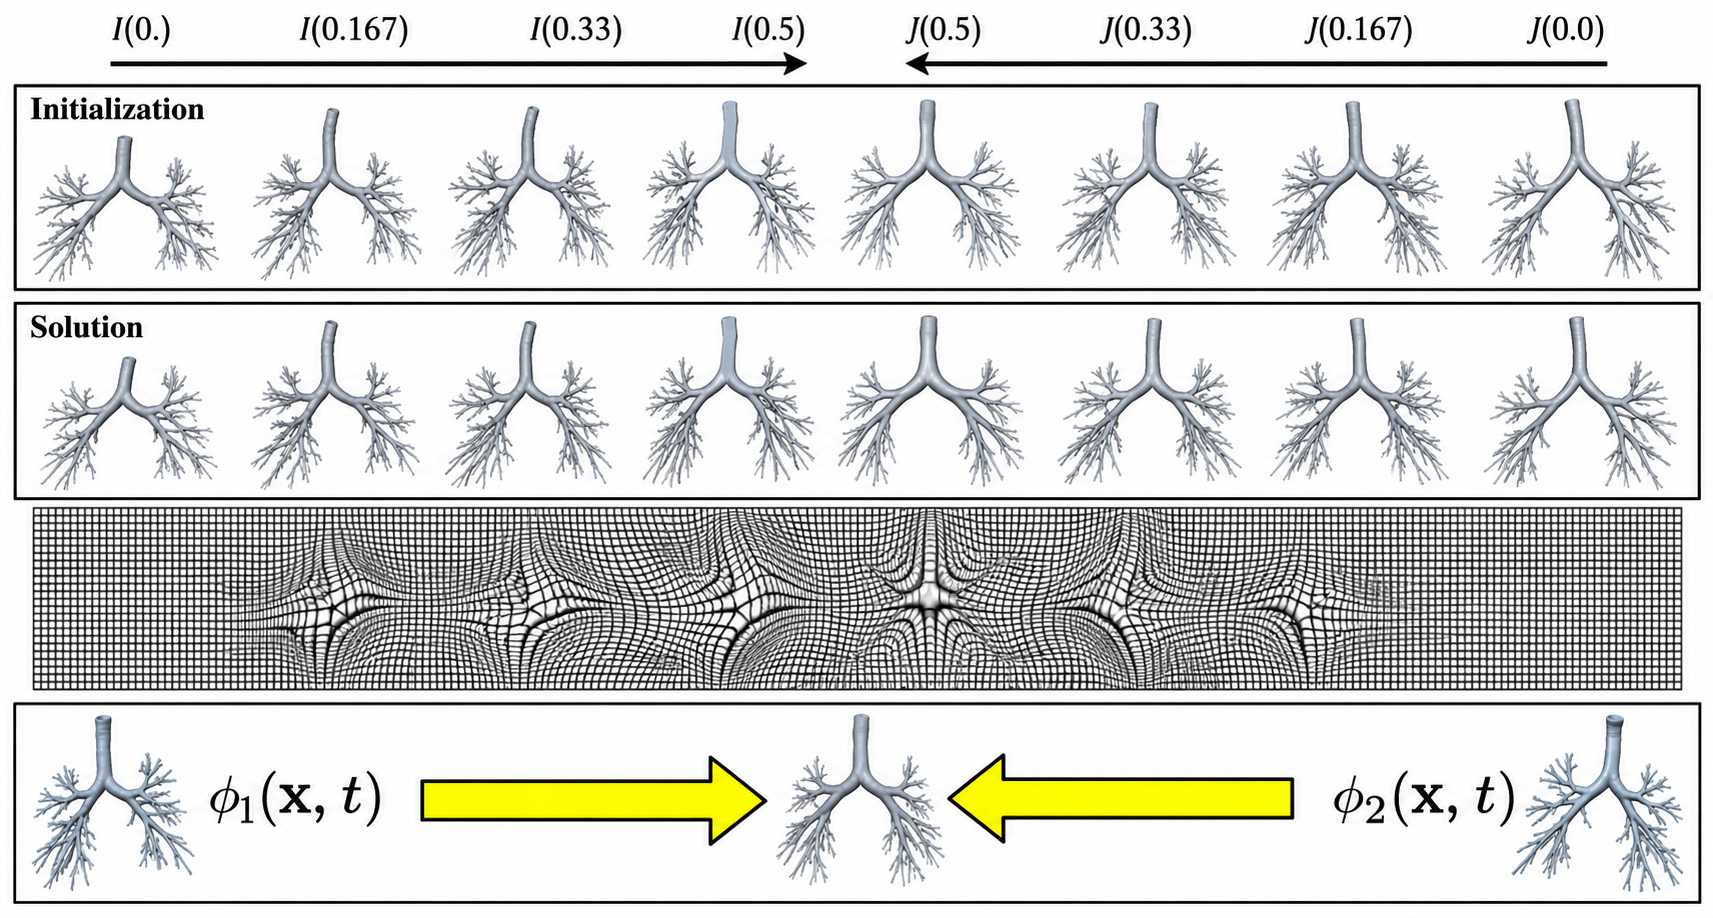
\includegraphics[width=\textwidth]{figures/syn_path_airways.png}  % the uploaded image
  \caption{Schematic of the symmetric SyN path between two airway trees $I$
  (left) and $J$ (right).
  Top: the two images at initialisation. Middle: after convergence, both
  images are deformed along $\phi_1$ and $\phi_2$ and meet at the mean shape
  at $t=0.5$. The full map from $I$ to $J$ is obtained by joining the two
  half-paths (Eq.~\ref{eq:syn_composition}). Illustrative only; not
  computed from the study data.}
  \label{fig:syn_path}                                 % referenced in the text above
\end{figure}

where $\Pi$ is a pointwise dissimilarity (the squared intensity difference in the
derivation of \citet{avants2008syn}, $-CC$ in their main method). The two
half-paths are kept at equal length, so both images travel the same distance and
meet at the \emph{mean shape} between them; SyN thus solves a two-image mean
problem, the pairwise counterpart of the template estimation in
\secref{sec:sygn}.

\paragraph{Full transformations by composition.}  % how the time-1 maps are obtained
The complete mapping between the two images is obtained by joining the
half-paths:
\begin{equation}
  \phi_1(\mathbf{x},1) = \phi_2^{-1}\big(\phi_1(\mathbf{x},0.5),\,0.5\big),
  \qquad
  \phi_1^{-1}(\mathbf{x},1) = \phi_1^{-1}\big(\phi_2(\mathbf{x},0.5),\,0.5\big).
  \label{eq:syn_composition}     % forward and inverse maps from the two halves
\end{equation}
Because $I$ and $J$ enter Eq.~\eqref{eq:syn_energy} in the same way, exchanging
them yields the same path in the opposite direction: the result does not depend
on which image is called ``fixed'' and which ``moving''.

\paragraph{Explicit, accurate inverses.}  % what distinguishes SyN from inverse-consistent methods
Diffeomorphisms are invertible in the continuous setting, but interpolation
errors in a discrete implementation accumulate and can break invertibility. SyN
therefore computes the inverses $\phi_i^{-1}$ explicitly with a fixed-point
algorithm and enforces $\phi_i^{-1}(\phi_i)=\mathrm{Id}$ and
$\phi_i(\phi_i^{-1})=\mathrm{Id}$ to sub-voxel accuracy. This distinguishes SyN
from inverse-consistent registration, in which forward and backward maps are
estimated separately and made consistent only approximately through penalty
terms. Both the subject-to-template and the template-to-subject mappings are
therefore available and consistent.

\paragraph{Optimisation in practice.}  % the algorithmic loop of one registration
Each SyN iteration deforms both images to the midpoint, computes the gradient of
the similarity term with respect to each half-map, smooths it into velocity
updates, updates $\phi_1$ and $\phi_2$ through a discretisation of
Eq.~\eqref{eq:syn_flow} with a sub-voxel step, recomputes the inverses and forms
the maps of Eq.~\eqref{eq:syn_composition}. The operator $L$ is approximated by a
Gaussian kernel applied to the \emph{incremental} update rather than to the total
displacement (\texttt{flow\_sigma} and \texttt{total\_sigma} in ANTsPy);
smoothing the increment is what permits large diffeomorphic deformations,
whereas smoothing the total displacement, as in elastic and Demons-type methods,
restricts the solution to small deformations. The optimisation runs from coarse
to fine resolution levels.
% TODO: current ANTs releases implement a greedy variant of SyN; cite the ANTs
% TODO: implementation paper if you want to state this explicitly.

% ==============================================================================
\subsubsection{Groupwise template construction with SyGN}
\label{sec:sygn}                 % the build_template loop

\paragraph{Formulation.}  % what SyGN optimises (avants2010sygn, Eq. 4)
SyGN seeks the template and the set of transformations that give the
``smallest'' parameterisation of the dataset, measured by the SyN energy of
Eq.~\eqref{eq:syn_energy}. The template is described by an appearance $\bar I$
(its intensities) and a shape, represented by a diffeomorphism $\psi$ that
defines the template's coordinate system. Given the images $\{J^i\}_{i=1}^N$,
\citet{avants2010sygn} minimise
\begin{equation}
  E_{\bar I} = \sum_{i=1}^{N} E_S\big(\bar I, J^i, \phi^i\big)
  \qquad\text{with}\qquad \phi^i(\mathbf{x},0) = \psi(\mathbf{x})\;\;\forall i,
  \label{eq:sygn_energy}         % sum of pairwise SyN energies, common starting point psi
\end{equation}
jointly over the mappings $\phi^i$, the appearance $\bar I$ and the shape $\psi$.
No initial template has to be chosen by the user, and the stated goals are that
the final template's appearance does not depend on any specific anatomy and its
shape does not depend on any individual's coordinate system.

\paragraph{Coordinate-descent algorithm.}  % the loop in the paper
Eq.~\eqref{eq:sygn_energy} is minimised by coordinate descent, one group of
variables at a time with the others fixed. After initialisation, each iteration
(1)~registers every image to the fixed template with SyN; (2)~updates the template
appearance $\bar I$; (3)~updates the template shape $\psi$ towards the average of
the mappings; and (4)~resamples the template through the new $\psi$, resets the
mappings to start from it, and repeats. The template is only updated after all
registrations of an iteration are complete, so appearance and shape are never
estimated from partially optimised mappings. \texttt{ants.build\_template}
implements the same loop, but with a different initialisation and a different
appearance update, as described next (figure~\ref{fig:sygn_paths}).

\begin{figure}[htbp]                                   % float near the SyGN loop
  \centering                                           % centre the image
  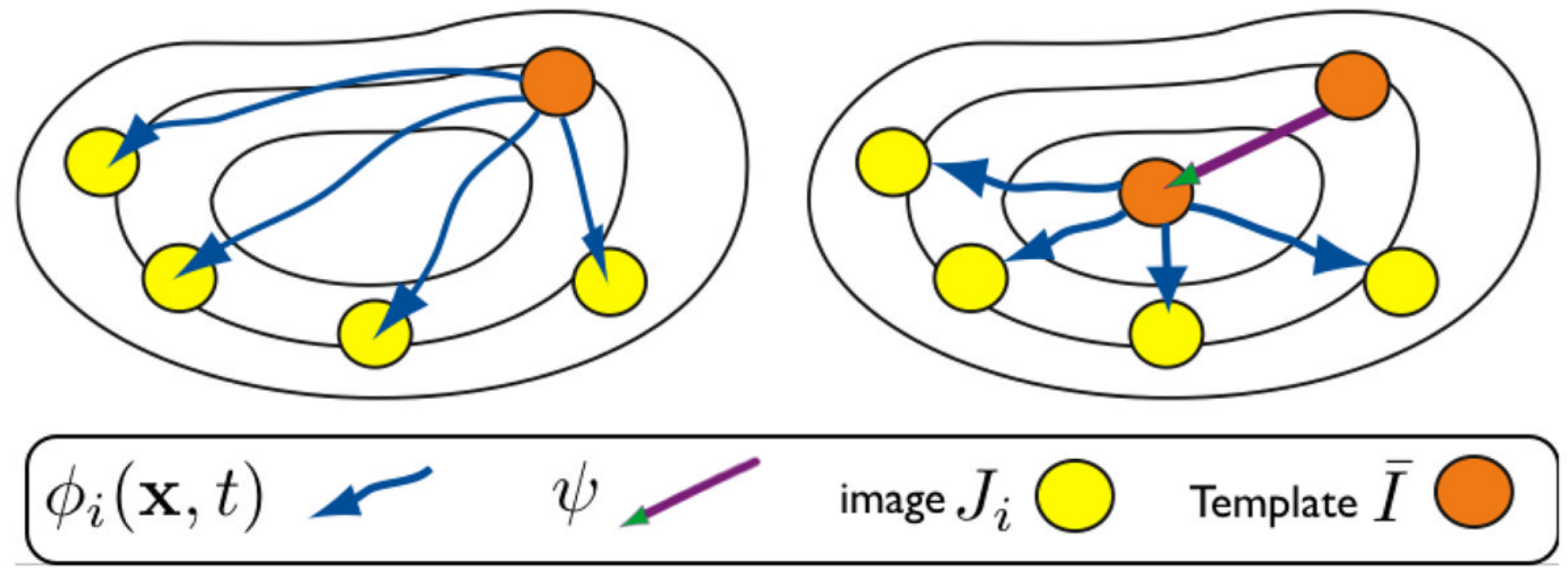
\includegraphics[width=0.8\textwidth]{figures/sygn_paths.png}  % Fig. 2 of avants2010sygn
  \caption{Two steps of one SyGN iteration. Left: the diffeomorphic paths
  $\phi_i$ from the current template $\bar I$ (orange) to the images $J_i$
  (yellow) are estimated (Step~1). Right: the template shape is moved by $\psi$
  towards the population centre, which shortens the total path length
  (Step~3). Reproduced from \citet{avants2010sygn}, Fig.~2.}
  \label{fig:sygn_paths}                               % referenced here and in Step 3
\end{figure}

\paragraph{Initialisation.}  % paper vs ANTsPy, and where the template grid comes from
In \citet{avants2010sygn}, the first template is the voxelwise (Euclidean)
average of the images \emph{after affine alignment}, and all $\phi^i$ and $\psi$
start as the identity. In the present implementation no initial template was
supplied, and ANTsPy forms the initial template \emph{without any alignment}: each
image is multiplied by its weight $w_i = 1/N$, resampled onto the voxel grid of
the first input image $I_1$, and summed,
\begin{equation}
  T^{(0)}(\mathbf{x}) = \sum_{i=1}^{N} w_i\, I_i(\mathbf{x}),
  \qquad \mathbf{x}\in\Omega_{I_1}.
  \label{eq:initial_template}    % unaligned mean, on the grid of the first image
\end{equation}
Two consequences follow. First, $T^{(0)}$ averages the airway trees as they lie
in their own scanner coordinates, so it is blurred and its quality depends on how
well these coordinate systems already agree. Because the inputs are binary
segmentations, it also contains intermediate values equal to the fraction of
volumes that contain airway at each location. Second, every later template is
resampled on this grid, so the origin, spacing, orientation and field of view of
the final template are inherited from $I_1$, here the first randomly selected
ATM'22 volume. The template's \emph{shape} is still optimised over the whole
population, but its \emph{grid} is not independent of the input order.

\paragraph{Step 1 -- registration.}  % links to the SyN subsection
With $T^{(k)}$ fixed, each $I_i$ is registered to it with the ANTsPy \texttt{SyN}
preset (\secref{sec:syn}), giving the affine maps $A_i^{(k)}$, the
deformable maps $\phi_i^{(k)}$ and the warped images
$I_i\circ\Phi_i^{(k)}$, all on the template grid.

\paragraph{Step 2 -- appearance update.}  % largest difference between paper and ANTsPy
\citet{avants2010sygn} do not take the template appearance to be a plain average.
They optimise it by gradient ascent on the cross-correlation of
Eq.~\eqref{eq:local_cc} between the template and the warped images (intensities
normalised to $[0,1]$, gradients smoothed with a Gaussian of $\sigma=1$ voxel,
step size $0.1$), and show that this preserves more contrast and detail than the
Euclidean mean. ANTsPy does \emph{not} implement this step. Its appearance is the
weighted Euclidean mean of the warped images,
\begin{equation}
  T_{\mathrm{avg}}^{(k+1)}(\mathbf{x})
  = \sum_{i=1}^{N} w_i \left[ I_i\circ\Phi_i^{(k)} \right]\!(\mathbf{x}),
  \label{eq:average_registered}  % mean of the aligned (warped) airway images
\end{equation}
and, at the end of each iteration (after the shape update below), this image is
blended with a sharpened copy of itself,
\begin{equation}
  T^{(k+1)} = \beta\, T^{(k+1)}_{\mathrm{shape}}
  + (1-\beta)\, \operatorname{Sharpen}\!\left(T^{(k+1)}_{\mathrm{shape}}\right),
  \label{eq:blending}            % 75% updated template + 25% sharpened template
\end{equation}
with $\beta=$ \texttt{blending\_weight} $=0.75$. The sharpening blend is a
heuristic of the implementation that compensates for the blurring of the mean; it
appears in neither publication and does not deform the template. In both the
paper and the implementation, averaging happens \emph{after} spatial alignment,
so each template location combines corresponding locations of the airway trees
rather than identical voxel indices of the original images.

\paragraph{Step 3 -- shape update.}  % Frechet mean of the diffeomorphisms
Averaging aligned images fixes the appearance but not the \emph{position} of the
template within the population: if the current template is closer to some
subjects than to others, the mappings to those subjects are short and the others
long (figure~\ref{fig:sygn_paths}, right). \citet{avants2010sygn} therefore move the template towards the Fréchet
(intrinsic) mean of the diffeomorphisms, the shape $\psi$ that minimises the total
squared geodesic distance $\sum_i D^2(\psi,\phi^i(\cdot,1))$ of
Eq.~\eqref{eq:shape_distance}. Velocity fields, unlike diffeomorphisms, can be
added, so the average can be taken over the initial velocity fields of the
mappings; setting the derivative of the total distance to zero gives the
optimality condition
\begin{equation}
  \bar{\mathbf{v}} = \sum_{i=1}^{N} \mathbf{v}^i(\psi,0) = 0,
  \label{eq:frechet_condition}   % template is at the mean when the mean velocity vanishes
\end{equation}
and, away from the optimum, the template shape evolves along
$d\psi/d\bar t = \bar{\mathbf{v}}(\psi,\bar t)$. Under a small-deformation
approximation, with $\psi=\mathrm{Id}$ at the current template, one step of
length $\Delta\bar t$ becomes a scaled sum of the displacements of the mappings:
\begin{equation}
  \psi_{\Delta\bar t}(\mathbf{x})
  = \mathbf{x} + \frac{\Delta\bar t}{\Delta t}
    \sum_{i=1}^{N} \big( \phi^i_1(\mathbf{x},\Delta t) - \mathbf{x} \big).
  \label{eq:shape_step}          % gradient step towards the average shape
\end{equation}
At the average configuration the displacements cancel and the template no longer
moves. ANTsPy implements this approximation: it averages the forward
displacement fields $W_i^{(k)}$ of the deformable registrations,
$W^{(k)}=\sum_i w_i W_i^{(k)}$, scales the result by $-\alpha$ with
$\alpha=$ \texttt{gradient\_step} $=0.2$ (the counterpart of $\Delta\bar t$),
combines it with the inverse of the average affine transformation
$\bar A^{(k)}$ of the registrations, and resamples the averaged image through the
resulting map $\Psi^{(k)}$:
\begin{equation}
  T^{(k+1)}_{\mathrm{shape}} = T_{\mathrm{avg}}^{(k+1)} \circ \Psi^{(k)},
  \qquad
  \Psi^{(k)} \;\text{built from}\; -\alpha\,W^{(k)} \;\text{and}\; \big(\bar A^{(k)}\big)^{-1}.
  \label{eq:shape_update}        % ANTsPy shape update (schematic)
\end{equation}
Two simplifications relative to the paper should be noted: ANTsPy averages total
displacement fields rather than initial velocity fields, and it also re-centres
the template affinely. With \texttt{useNoRigid=True} (the default), the rigid
part is excluded from $\bar A^{(k)}$, so only the average scaling and shear are
removed and the template does not drift by an arbitrary common rotation or
translation. Eq.~\eqref{eq:shape_update} is schematic; the exact composition
order follows the ANTsPy source.

\paragraph{Why the shape update matters for segmentation volumes.}  % Fig. 3 of avants2010sygn
\citet{avants2010sygn} illustrate this step (Figure~\ref{fig:sygn_ellipses}) with a synthetic set of four binary
ellipses with the same centre and different radii. The initial average has
intermediate grey levels, like the averaged airway masks here. With the shape
update, SyGN converges, up to interpolation error, to the true mean shape. Without
it, optimising appearance alone converges to a geometrically wrong template, the
$0.5$ level set of the initial average. The shape update is therefore what makes
the geometry of a template built from binary segmentations reflect the population
average rather than the initialisation; setting \texttt{gradient\_step} $>0$ is
essential for this.

\begin{figure}[htbp]                                   % float near the shape-update argument
  \centering                                           % centre the image
  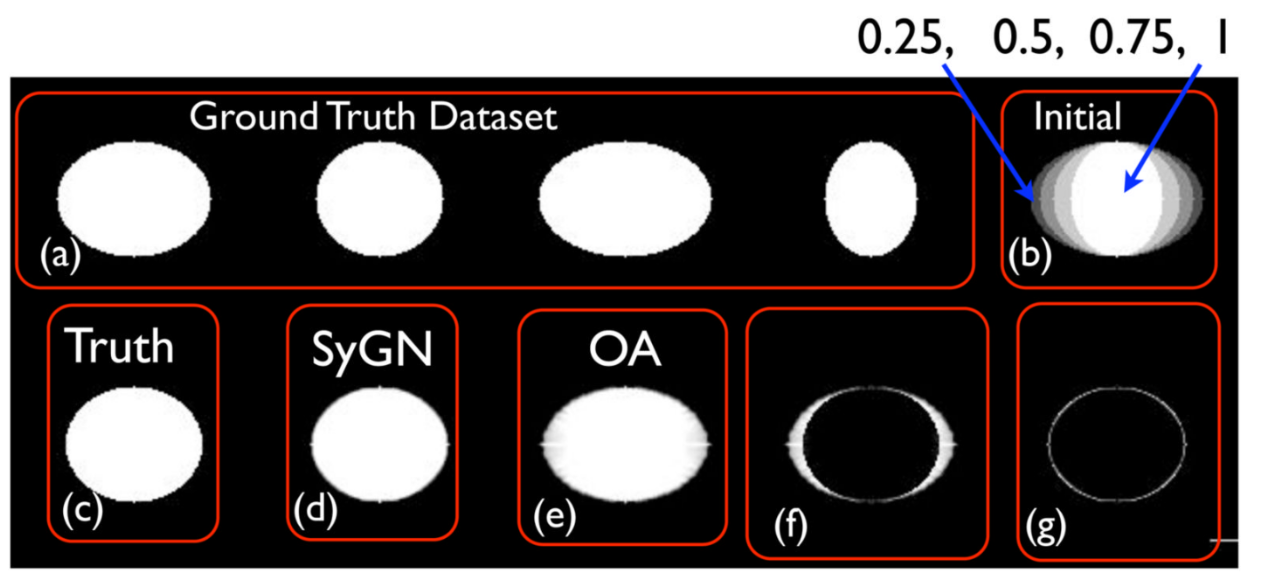
\includegraphics[width=0.8\textwidth]{figures/sygn_ellipses.png}  % Fig. 3 of avants2010sygn
  \caption{Effect of the shape update on binary images. (a)~Four binary
  ellipses; (b)~their initial average, with grey levels $0.25$--$1$;
  (c)~true mean shape; (d)~SyGN result with shape update; (e)~result without
  shape update (appearance only), which converges to the wrong shape;
  (f,g)~errors of (e) and (d) with respect to (c). Reproduced from
  \citet{avants2010sygn}, Fig.~3.}
  \label{fig:sygn_ellipses}                            % referenced in the paragraph above
\end{figure}

\paragraph{Iterations and convergence.}  % how many loops and how to check them
The loop was run for a fixed number of $8$ iterations (the ANTsPy default is
$3$). \citet{avants2010sygn} report that SyGN typically converges in fewer than
ten iterations, usually three to five, depending on the complexity of the
deformations. No stopping criterion is applied by the code. However, ANTsPy
prints the mean absolute value of the average displacement field $W^{(k)}$ at
every iteration; by Eq.~\eqref{eq:frechet_condition} this quantity should tend
towards zero as the template approaches the population mean, and it can be used
to assess convergence.
% TODO: report the 8 printed values of mean |W| from the log (table or plot),
% TODO: e.g. "decreased from ... mm to ... mm", to support the choice of 8 iterations.

\paragraph{Unbiasedness and its limits.}  % what the claims mean for this run
In principle SyGN gives a template that is unbiased: it requires no
user-selected reference, uses a symmetric pairwise method, and centres the
template shape on the population. In the present implementation this holds for
the template shape up to three qualifications: the template grid is inherited
from the first input volume (Eq.~\eqref{eq:initial_template}); the eight volumes
are a small random subset of the two datasets; and the registrations and the
appearance use MI and a sharpened mean instead of the cross-correlation model of
the reference publications.

\paragraph{Output.}  % what the code writes
After the eighth iteration, the template $T^{(8)}$ was written to
\texttt{template.nii.gz}. It is the reference used in
\secref{sec:affine}. The complete procedure is summarised in
Figure~\ref{fig:template_pipeline}.

\begin{figure}[htbp]             % float: LaTeX picks the best spot
  \centering                     % centre the diagram
  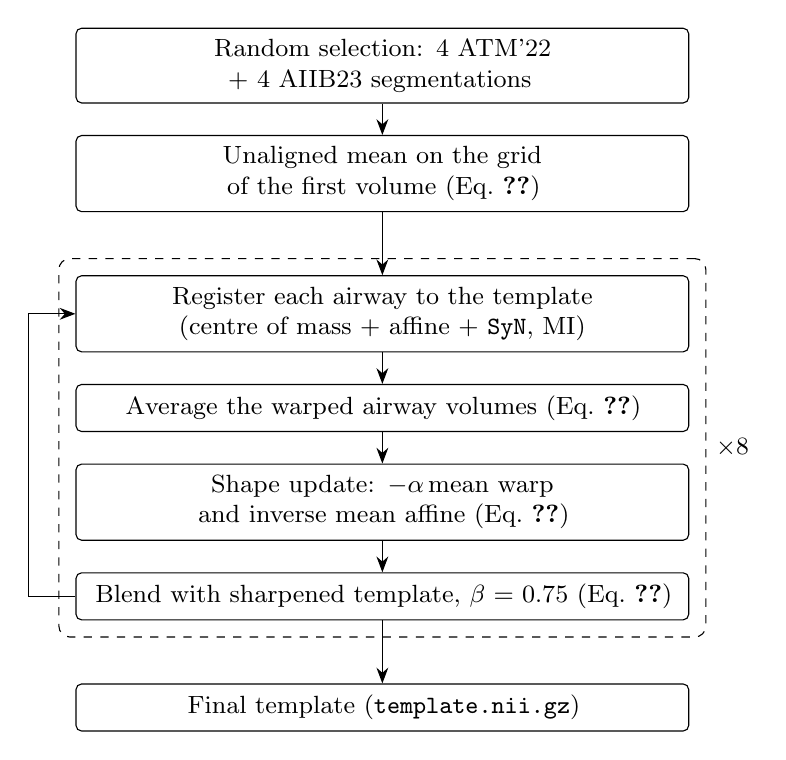
\begin{tikzpicture}[
      node distance=4mm,                                 % vertical gap between steps
      box/.style={draw, rounded corners=2pt, align=center,
                   text width=7.5cm, inner sep=4pt, font=\small},  % one box per step
      arr/.style={-{Stealth[length=2mm]}}]               % arrow style
    \node[box]                        (in)   {Random selection: 4 ATM'22 + 4 AIIB23 segmentations};
    \node[box, below=of in]           (init) {Unaligned mean on the grid of the first volume (Eq.~\ref{eq:initial_template})};
    \node[box, below=8mm of init]     (reg)  {Register each airway to the template\\(centre of mass + affine + \texttt{SyN}, MI)};
    \node[box, below=of reg]          (avg)  {Average the warped airway volumes (Eq.~\ref{eq:average_registered})};
    \node[box, below=of avg]          (shp)  {Shape update: $-\alpha\,$mean warp and inverse mean affine (Eq.~\ref{eq:shape_update})};
    \node[box, below=of shp]          (bld)  {Blend with sharpened template, $\beta=0.75$ (Eq.~\ref{eq:blending})};
    \node[draw, dashed, rounded corners=4pt, inner sep=6pt,
          fit=(reg)(bld), label={[font=\small\itshape]right:$\times 8$}] (loop) {};  % the iteration block
    \node[box, below=8mm of bld]      (tpl)  {Final template (\texttt{template.nii.gz})};
    \foreach \a/\b in {in/init, init/reg, reg/avg, avg/shp, shp/bld, bld/tpl}
      \draw[arr] (\a) -- (\b);                           % straight arrows down the chain
    \draw[arr] (bld.west) -- ++(-6mm,0) |- (reg.west);   % loop back: next iteration
  \end{tikzpicture}
  \caption{Groupwise template construction with \texttt{ants.build\_template}.
  The dashed block is one SyGN iteration, repeated eight times.}
  \label{fig:template_pipeline}  % referenced in the Output paragraph
\end{figure}

The NIfTI geometry defines where each original voxel grid lies in physical
space, whereas the affine and diffeomorphic transformations estimated by ANTs
establish anatomical correspondence between these physical domains. The final
template is therefore a population-derived coordinate space in which the
anatomical variability of the eight airway trees has been brought into
correspondence.
  % Subsection "Template construction"
% Affine registration -- mapping individual airway trees to the finished template.
% Subsection of "Registration", pulled in by sections/04-registration.tex.

% ==============================================================================
\subsection{Affine registration}
\label{sec:affine}               % target of \secref{sec:affine} in the template section

% % Affine registration -- version written with ChatGPT.
% Pulled in by sections/registration/affine-registration.tex.

\subsubsection{ChatGPT}          % second version of the affine-registration text
\label{sec:affine_chatgpt}       % \secref{sec:affine_chatgpt}

Following template construction, the airway segmentation volumes were spatially
aligned to a common anatomical reference using affine image registration. The
registration was performed using the Advanced Normalization Tools (ANTs)
framework through its Python interface, ANTsPy. ANTs is an open-source
framework for quantitative medical image analysis whose core functionality
includes image registration and template construction
\cite{avants2009ants,tustison2021antsx}. For each subject, the corresponding
three-dimensional airway segmentation volume from the AIIB23 dataset was
considered as the \emph{moving} image, whereas the previously constructed
airway template, \texttt{template\_22.nii.gz}, was used as the \emph{fixed}
image. In the implemented pipeline, all available input volumes were processed
independently and registered to this fixed reference.

% ------------------------------------------------------------
\paragraph{Affine transformation.}  % definition of the affine map

The affine registration models global geometric differences between an
individual airway tree and the reference template. In three-dimensional
space, an affine transformation can be written as
\begin{equation}
  \mathbf{x}' = \mathbf{A}\mathbf{x} + \mathbf{t},
  \label{eq:affine_transform}    % linear part A plus translation t
\end{equation}
where $\mathbf{x} \in \mathbb{R}^{3}$ denotes a point in the original image
space, $\mathbf{x}' \in \mathbb{R}^{3}$ its transformed position,
$\mathbf{A} \in \mathbb{R}^{3\times3}$ is the linear component of the
transformation, and $\mathbf{t} \in \mathbb{R}^{3}$ is the translation
vector. The matrix $\mathbf{A}$ can represent rotation, scaling, and shearing,
whereas $\mathbf{t}$ accounts for translation
\cite{itk_software_guide}. Consequently, a three-dimensional affine
transformation contains twelve parameters, corresponding to the nine elements
of the linear transformation matrix and the three translation parameters. The
ANTsPy documentation explicitly defines its \texttt{Affine} registration
option as an affine transformation with 12 parameters
\cite{antspy_registration}.

In contrast to deformable registration, the affine transformation is global:
the same transformation is applied throughout the image. It can therefore
correct subject-specific differences in overall position, orientation, scale,
and global shear, but it does not introduce spatially varying local
deformations. Consequently, the relative geometric configuration of the
airway tree is preserved while the tree is brought into a common global
coordinate system \cite{itk_software_guide,avants2009ants}.

% ------------------------------------------------------------
\paragraph{Registration as an optimization problem.}  % transform + metric + optimiser

Let $F$ denote the fixed template and $M$ the moving subject image. The
registration seeks the affine transformation parameters
$\boldsymbol{\theta}$ that optimize a similarity-based registration objective
between the fixed image and the transformed moving image. In general, the
registration problem can be expressed as
\begin{equation}
  \boldsymbol{\theta}^{*}
  = \underset{\boldsymbol{\theta}}{\operatorname{arg\,opt}}\;
  \mathcal{C}\left(F,\, M \circ T_{\boldsymbol{\theta}}\right),
  \label{eq:registration_optimization}  % optimise the objective over the affine parameters
\end{equation}
where $T_{\boldsymbol{\theta}}$ is the affine transformation parameterized by
$\boldsymbol{\theta}$, $M \circ T_{\boldsymbol{\theta}}$ denotes the moving
image after transformation, and $\mathcal{C}$ denotes the registration
objective. Image registration frameworks such as ITK formulate registration
through the combination of a transformation model, a similarity metric, and
an optimization procedure \cite{itk_software_guide,avants2014itkv4}.

In the present implementation, the registration is invoked through the ANTsPy
interface as

\begin{lstlisting}
ants.registration(
    fixed=fixed,
    moving=moving,
    type_of_transform='Affine'
)
\end{lstlisting}

\noindent where the fixed image is the image defining the reference space and
the moving image is the image mapped to that space \cite{antspy_registration}.
The choice \texttt{type\_of\_transform='Affine'} therefore specifies that the
estimated transformation belongs to the affine transformation family rather
than to a deformable model.

The implementation does not explicitly specify additional registration
parameters such as the similarity metric, optimization schedule, number of
iterations, or multiresolution settings. These are therefore determined by
the ANTsPy \texttt{Affine} registration preset associated with the software
version used in the experiment. The ANTsPy documentation exposes these
parameters explicitly, including the affine metric, sampling strategy,
iteration schedule, shrink factors, and smoothing sigmas
\cite{antspy_registration}. This distinction is important for reproducibility:
only parameters explicitly specified in the experimental code should be
reported as manually selected parameters.

% ------------------------------------------------------------
\paragraph{Mapping and resampling to template space.}  % from transform to output volume

After estimating the affine transformation, the transformed moving image is
resampled onto the spatial domain of the fixed image. In the ITK registration
framework, the moving image is evaluated at the physical coordinates induced
by the estimated transformation, and an interpolator is used when mapped
locations do not coincide with the original voxel grid
\cite{itk_software_guide}. The purpose of this resampling step is to obtain a
representation of the moving image on the grid of the fixed image, allowing
the registered volumes to share a common spatial reference.

In the implemented pipeline, the registered volume is obtained from the
\texttt{warpedmovout} output returned by \texttt{ants.registration}. According
to the ANTsPy documentation, \texttt{warpedmovout} is the moving image warped
into the space of the fixed image \cite{antspy_registration}. The resulting
volume is subsequently written as a new NIfTI file, thereby producing an airway
segmentation expressed in the coordinate system of the template.

The complete procedure can therefore be summarized as
\begin{equation}
  \begin{split}
    &\text{subject airway segmentation}
     \;\xrightarrow{\text{affine registration}}\;
     \text{estimated affine transformation} \\
    &\qquad\xrightarrow{\text{resampling}}\;
     \text{registered segmentation in template space}.
  \end{split}
  \label{eq:affine_pipeline}     % split over two lines so it fits the page width
\end{equation}

The resulting registered airway volumes share a common spatial reference and
can consequently be used for subsequent inter-subject analysis, including
morphological comparison, shape analysis, and representation learning.

% ------------------------------------------------------------
\paragraph{Implementation and computational setup.}  % parallel execution and outputs

The registration was applied independently to all available AIIB23 airway
segmentation volumes. The implementation uses a parallelized execution
strategy, with 12 registration jobs and 4 ITK threads assigned to each job.
These settings concern the computational execution of the pipeline and do not
change the mathematical definition of the affine transformation itself.

The registered volumes were saved in the specified output directory using the
subject identifier followed by the suffix \texttt{\_R.nii.gz}. These files
represent the final airway segmentations after affine alignment to the common
template and were used as inputs to the subsequent processing stages.
  % Subsubsection "ChatGPT"


% --- Values to fill in (shown in red in the PDF until replaced) ---
\newcommand{\ncases}{\TODO{N}}                % number of AIIB23 segmentations registered
\newcommand{\antspyversion}{\TODO{x.y.z}}     % python -c "import ants; print(ants.__version__)"

Airway trees extracted from different patients differ in position, orientation
and overall size, as a consequence of patient positioning in the scanner,
differences in body size and acquisition parameters. To make them directly
comparable, all airway segmentations were mapped into the constructed template.
 An affine transformation was chosen for this purpose because it compensates for these global differences
while preserving the local geometry of each airway tree, which is the object of
the subsequent analysis.

Affine registration consists of finding the spatial transformation $T$ that best aligns
a \emph{moving} image $M$ with a \emph{fixed} image $F$. In this work, the fixed
image is the template and each AIIB23 segmentation is, in turn, the moving
image. The transformation is restricted to the class of three-dimensional affine
maps,
\begin{equation}
  T_{\boldsymbol{\mu}}(\mathbf{x}) = \mathbf{A}\,(\mathbf{x} - \mathbf{c}) + \mathbf{c} + \mathbf{t},
  \label{eq:affine}              % affine map: linear part A plus translation t
\end{equation}
where $\mathbf{x} \in \mathbb{R}^3$ is a point in the fixed image domain,
$\mathbf{A} \in \mathbb{R}^{3\times 3}$ is a general matrix,
$\mathbf{t} \in \mathbb{R}^3$ is a translation vector and $\mathbf{c}$ is a
fixed centre of rotation. The parameter vector $\boldsymbol{\mu}$ therefore
contains $9 + 3 = 12$ degrees of freedom, which jointly encode translation,
rotation, anisotropic scaling and shear. Because the transformation is linear up
to a translation, straight lines are mapped to straight lines and parallelism is
preserved, so the shape of the airway tree is modified only globally.

% ------------------------------------------------------------
\paragraph{Similarity metric and optimisation.}  % what is optimised and how

The optimal parameters are obtained by solving
\begin{equation}
  \hat{\boldsymbol{\mu}} = \arg\min_{\boldsymbol{\mu}} \;
  \mathcal{C}\big(F,\, M \circ T_{\boldsymbol{\mu}}\big),
  \label{eq:optimisation}        % registration as an optimisation problem
\end{equation}
where $\mathcal{C}$ is a cost function measuring the dissimilarity between the
fixed image and the transformed moving image. The cost function used is the
negative of the Mattes mutual information \cite{mattes2003petct},
\begin{equation}
  \mathcal{C}(\boldsymbol{\mu}) = -\sum_{\iota}\sum_{\kappa} p(\iota,\kappa;\boldsymbol{\mu})
  \log \frac{p(\iota,\kappa;\boldsymbol{\mu})}{p_F(\iota)\, p_M(\kappa;\boldsymbol{\mu})},
  \label{eq:mattes}              % negative mutual information from the joint histogram
\end{equation}
where $p(\iota,\kappa;\boldsymbol{\mu})$ is the joint probability of intensity
bins $\iota$ and $\kappa$ in the fixed and transformed moving images, and $p_F$
and $p_M$ are the corresponding marginal distributions. In the Mattes
formulation, these distributions are estimated with B-spline Parzen windows,
which makes the metric differentiable with respect to $\boldsymbol{\mu}$. The
histograms were built with 32 bins from a random sample of 20\% of the voxels,
which reduces the computational cost of each iteration.

Equation~\eqref{eq:optimisation} was solved with a gradient descent optimiser.
Before optimisation, the transformation was initialised by aligning the
intensity centres of mass of the two images, which provides a coarse
translational alignment and reduces the risk of convergence to a poor local
optimum.

% ------------------------------------------------------------
\paragraph{Multi-resolution strategy.}  % coarse-to-fine scheme

To improve robustness and speed, the optimisation was performed within a
four-level multi-resolution scheme \cite{thevenaz1998pyramid}. At each level,
both images were smoothed with a Gaussian kernel and downsampled by an integer
shrink factor; the optimisation then proceeded from the coarsest level to the
original resolution, with the result of each level used to initialise the next.
Coarse levels capture the large-scale alignment, while finer levels refine it.
The settings of each level are listed in Table~\ref{tab:multires}.

\begin{table}[htbp]              % per-level settings of the multi-resolution pyramid
  \centering                     % centre the table on the page
  \caption{Multi-resolution settings of the affine registration.}
  \label{tab:multires}           % referenced in the text above
  \begin{tabular}{cccc}          % four centred columns
    \toprule
    Level & Shrink factor & Gaussian $\sigma$ (voxels) & Maximum iterations \\
    \midrule
    1 (coarsest) & 6 & 3 & 2100 \\
    2            & 4 & 2 & 1200 \\
    3            & 2 & 1 & 1200 \\
    4 (finest)   & 1 & 0 & 10   \\
    \bottomrule
  \end{tabular}
\end{table}

At each level, the optimisation stopped either when the maximum number of
iterations was reached or when the cost function had converged, i.e.\ when its
variation over the last 10 iterations fell below $10^{-6}$.

% ------------------------------------------------------------
\paragraph{Resampling of the registered images.}  % how outputs were produced

Once the optimal transformation $T_{\hat{\boldsymbol{\mu}}}$ had been estimated,
each moving segmentation was resampled onto the voxel grid of the template using
linear interpolation and saved in NIfTI format. Since the inputs are binary
masks, linear interpolation yields intermediate values in $[0,1]$ at the
boundary of the airway lumen, while voxels well inside or outside the airway
keep the values 1 and 0 respectively.
% TODO: if the outputs were thresholded afterwards (e.g. at 0.5), state it here.

% % ------------------------------------------------------------
% \paragraph{Implementation.}      % software and computing environment

% The registration was implemented in Python~3.11 with ANTsPy (version
% \antspyversion) \cite{tustison2021antsx}, the Python interface of the Advanced
% Normalization Tools (ANTs) \cite{avants2009ants}, which is built on the
% registration framework of the Insight Toolkit (ITK) \cite{avants2014itkv4}. The
% affine registration was obtained with the function \texttt{ants.registration}
% using the predefined \texttt{Affine} transformation type, whose default settings
% correspond to the parameters described above under \emph{Similarity metric and
% optimisation} and \emph{Multi-resolution strategy}.

% Since each segmentation is registered to the template independently of the
% others, the task is embarrassingly parallel. The computation was run on a single
% node of a high-performance computing cluster managed by the SLURM workload
% manager \cite{yoo2003slurm}, with 48 CPU cores and 128\,GB of memory allocated
% to the job. Parallelism was organised on two levels: the joblib library
% \cite{joblib} distributed the registrations over 12 independent worker
% processes, and each registration used 4 ITK threads, so that
% \begin{equation}
%   12 \text{ processes} \times 4 \text{ threads} = 48 \text{ cores},
%   \label{eq:cores}               % total cores used = processes x threads per process
% \end{equation}
% matching the allocated resources exactly. Segmentations for which a registered
% output already existed were skipped, which allowed an interrupted job to be
% resumed without repeating completed registrations.

% Because the similarity metric is estimated from a random subset of voxels and no
% fixed random seed was set, repeating a registration may yield slightly different
% transformation parameters; these differences are expected to be small relative
% to the global misalignment corrected by the affine transformation.
    % Subsection "Affine registration"          % Registration: Template construction + Affine registration
% Encoding -- parent section; each approach is a subsection in its own file.

\section{Encoding}               % learning a compact representation of each airway tree
\label{sec:encoding}             % \secref{sec:encoding}

\hint{Optional short introduction: why a learned representation of the airway trees is
needed, and the three approaches tried -- a variational autoencoder, deterministic and
sparse autoencoders, and an implicit encoding.}

% Variational autoencoder -- subsection of "Encoding", pulled in by sections/05-encoding.tex.
% Red \TODO{...} marks replace the [square-bracket] placeholders of the original draft.

\subsection[Variational autoencoder]{Variational Autoencoder for Airway Tree Representation Learning}
\label{sec:vae}                          % \secref{sec:vae}

% ------------------------------------------------------------------------------
\subsubsection{Motivation}               % why a VAE is used
\label{sec:vae_motivation}               % \secref{sec:vae_motivation}

To learn a compact representation of airway trees, we represent each tree as a binary
voxel occupancy grid. As \citet{brock2016} point out, there is no meaningful way
to interpolate directly between two binary grids. Relating voxelized shapes to one another
therefore requires a model that works in an abstract feature space capturing the main
factors of variation.

For this reason we use a Variational Autoencoder (VAE) \cite{kingma2014}. A VAE is a
probabilistic framework that learns two networks jointly:
\begin{itemize}                          % the two VAE components
  \item an \textbf{inference (encoder) network}, which maps an input to a set of latent
        variables describing it, and
  \item a \textbf{generative (decoder) network}, which maps from the latent space back to
        the input space.
\end{itemize}

Once the encoder has learned latent variables that describe the underlying variation between
shapes, each airway tree can be encoded as a latent vector. That vector can be used as a
learned representation, or interpolated and decoded back into a voxel grid. Our models
are adapted from the voxel-based VAE of \citet{brock2016}.

% ------------------------------------------------------------------------------
\subsubsection{Model architecture}       % encoder, latent layer, decoder for both resolutions
\label{sec:vae_architecture}             % \secref{sec:vae_architecture}

\paragraph{Input resolutions.}           % the two voxel grids used
Each airway tree was voxelized into a binary occupancy grid at two resolutions,
$128\times128\times128$ and $256\times256\times256$ voxels. The higher resolution preserves
more of the thin distal branches, at the cost of a much larger memory and computational
footprint. We trained a separate VAE for each resolution. Both networks follow the design
principles of \citet{brock2016}, adapted to the larger input size. The
$256^3$ model has one additional downsampling stage (two extra encoder layers), so that both
networks reach the same $7\times7\times7$ spatial grid at the bottleneck. The architectures
are summarized in Figure~\ref{fig:vae_arch} and Table~\ref{tab:vae_layers}.

\paragraph{Encoder.}                     % conv blocks, strided downsampling, channel growth
The encoder is a stack of 3D convolutional blocks. Each block consists of a
$3\times3\times3$ convolution without bias, instance normalization with learnable affine
parameters, and an ELU activation. As in \citet{brock2016}, downsampling is
performed with strided convolutions rather than pooling, in every second layer. The layers
alternate between an unpadded stride-1 convolution, which reduces each spatial dimension by
2, and a stride-2 convolution with padding 1, which approximately halves it. The number of
filters doubles at every layer:
\begin{itemize}                          % per-resolution encoder details
  \item \textbf{$128^3$ model:} 8 convolutional layers, starting with 2 filters and reaching
        256 filters. The spatial size goes
        $128 \to 126 \to 63 \to 61 \to 31 \to 29 \to 15 \to 13 \to 7$.
  \item \textbf{$256^3$ model:} 10 convolutional layers, starting with 4 filters and reaching
        2048 filters. The spatial size goes
        $256 \to 254 \to 127 \to 125 \to 63 \to 61 \to 31 \to 29 \to 15 \to 13 \to 7$.
\end{itemize}
A $1\times1\times1$ convolution (followed by instance normalization and ELU) then reduces the
number of channels to 32 while keeping the $7^3$ grid. The result is flattened into a vector
of $32 \cdot 7^3 = 10{,}976$ features. In \citet{brock2016}, a fully connected
layer is placed between the convolutional features and the latent projection. In our models
this layer is removed, and the flattened features are mapped directly by two separate linear
layers to the mean $\boldsymbol{\mu}$ and the log standard deviation $\log\boldsymbol{\sigma}$
of the latent Gaussian, of dimension \TODO{100}. The log standard deviation is clamped to
$[-10, 10]$ for numerical stability.

\paragraph{Latent sampling.}             % reparameterization during training vs. inference
During training, a latent vector is sampled with the reparameterization
trick \cite{kingma2014},
\begin{equation}
  \mathbf{z} = \boldsymbol{\mu} + \exp(\log\boldsymbol{\sigma}) \odot \boldsymbol{\epsilon},
  \qquad \boldsymbol{\epsilon} \sim \mathcal{N}(\mathbf{0}, \mathbf{I}).
  \label{eq:reparam}                     % reparameterization with log-sigma parameterization
\end{equation}
At inference time the mean is used directly ($\mathbf{z} = \boldsymbol{\mu}$), giving a
deterministic encoding of each airway tree.

\paragraph{Decoder.}                     % mirrored decoder with resize-convolution upsampling
The decoder mirrors the encoder, and its weights are not tied to the encoder's. A linear
layer maps $\mathbf{z}$ back to 10,976 features, followed by layer
normalization \cite{ba2016} and ELU, and the result is reshaped into a $32\times7^3$ volume.
A stride-1 convolutional block expands the channels to the width of the deepest encoder layer
(256 for the $128^3$ model, 2048 for the $256^3$ model). The decoder then alternates between
upsampling blocks and stride-1 convolutional blocks (padding 1, spatial size preserved),
halving the number of channels at every layer.

\citet{brock2016} upsample with fractionally strided (transposed) convolutions.
We instead use a resize-convolution: each upsampling block applies nearest-neighbour
upsampling to an exact target size, followed by a $3\times3\times3$ convolution, instance
normalization and ELU. This avoids the checkerboard artifacts associated with transposed
convolutions \cite{odena2016} and lets the decoder match the odd intermediate sizes of the
encoder (15, 31, 63, 127) exactly. The spatial size goes
$7 \to 15 \to 31 \to 63 \to 128$ for the $128^3$ model and
$7 \to 15 \to 31 \to 63 \to 127 \to 256$ for the $256^3$ model.

A final $3\times3\times3$ convolution with bias maps the features to a single output channel,
with no normalization or activation. Its outputs are logits; the sigmoid applied inside the
loss converts them into the predicted probability that each voxel is occupied.

\paragraph{Normalization, activations and initialization.}  % departures from the original
All layers use the ELU activation \cite{clevert2016}, except the output layer. Where Brock et
al.\ use Batch Normalization \cite{ioffe2015}, we use instance
normalization \cite{ulyanov2016}. At $128^3$ and $256^3$ resolution, GPU memory limits the
batch size to a few samples, which makes batch statistics unreliable; instance normalization
normalizes each sample independently and does not depend on batch size. Convolutional and
linear weights are initialized with Glorot (Xavier) normal initialization \cite{glorot2010},
and biases are initialized to zero.

\begin{table}[htbp]                      % layer-by-layer summary of both models
  \centering                             % center the table
  \small                                 % slightly smaller font so the table fits
  \caption{Summary of the two VAE architectures.}
  \label{tab:vae_layers}                 % referenced as Table~\ref{tab:vae_layers}
  \begin{tabular}{lcc}                   % 3 columns: stage, 128 model, 256 model
    \toprule
    Stage & $128^3$ model & $256^3$ model \\
    \midrule
    Input & $1 \times 128^3$ & $1 \times 256^3$ \\
    Encoder conv layers & 8 & 10 \\
    Filters (first $\to$ last) & $2 \to 256$ & $4 \to 2048$ \\
    Encoder output & $256 \times 7^3$ & $2048 \times 7^3$ \\
    $1\times1\times1$ reduction & $32 \times 7^3$ & $32 \times 7^3$ \\
    Flattened features & 10,976 & 10,976 \\
    Latent dimension & \TODO{100} & \TODO{100} \\
    Decoder upsampling steps & 4 & 5 \\
    Decoder filters (first $\to$ last) & $256 \to 2$ & $2048 \to 4$ \\
    Output & $1 \times 128^3$ (logits) & $1 \times 256^3$ (logits) \\
    \bottomrule
  \end{tabular}
\end{table}

\begin{figure}[htbp]                     % placeholder for the architecture diagram
  \centering                             % center the figure
  % 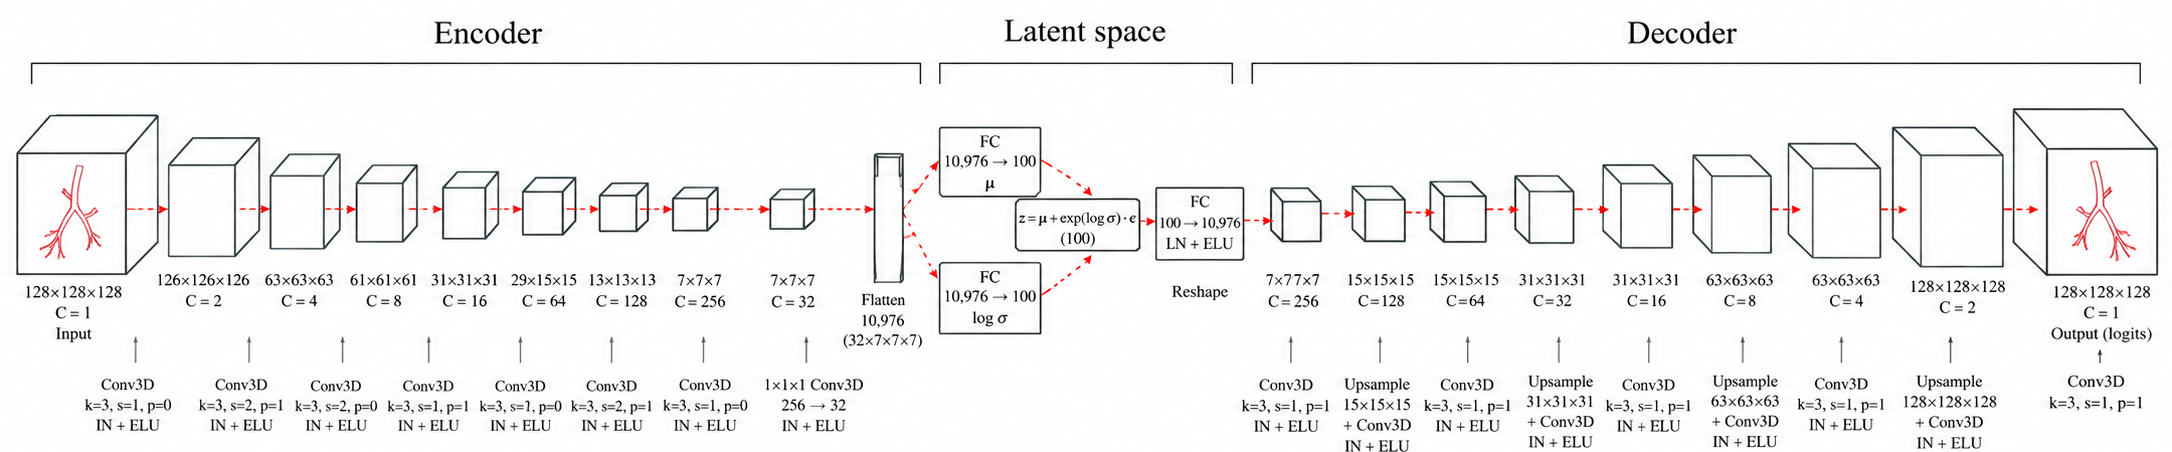
\includegraphics[width=\textwidth]{figures/vae_architecture.png}  % uncomment with your file
  \fbox{\parbox[c][4cm][c]{0.9\textwidth}{\centering [VAE architecture figure]}}  % remove once image added
  \caption{Architecture of the voxel-based VAEs, adapted from \citet{brock2016}. Shown for
           the $256^3$ model; the $128^3$ model omits the first downsampling stage.}
  \label{fig:vae_arch}                   % referenced as Figure~\ref{fig:vae_arch}
\end{figure}

% ------------------------------------------------------------------------------
\subsubsection{Loss function}            % BCE modification, KL, L2, clDice
\label{sec:vae_loss}                     % \secref{sec:vae_loss}

Following \citet{brock2016}, the loss combines three terms: the KL divergence
between the approximate posterior and the prior on the latent variables, L2 weight
regularization, and a reconstruction term based on a modified Binary Cross-Entropy (BCE).
We then add a fourth term, clDice, described below.

\paragraph{Modified BCE.}                % why and how the BCE is modified
The standard BCE is
\begin{equation}
  \mathcal{L}_{\mathrm{BCE}} = -t\log(o) - (1-t)\log(1-o),
  \label{eq:bce}                         % standard binary cross-entropy
\end{equation}
where $t \in \{0,1\}$ is the target voxel value and $o \in (0,1)$ is the network output.
\citet{brock2016} identify two problems with this loss for voxel data. First, its
derivative with respect to $o$ becomes very small as $o$ approaches $t$, which can cause
vanishing gradients. Second, it penalizes false positives and false negatives equally. Most
of a voxel grid is empty, so the network can fall into a poor local optimum by predicting
every voxel as empty. The second problem is even more severe for airway trees than for the
ModelNet objects in the original paper: airways are thin, branching structures that occupy a
very small fraction of the grid.

\citet{brock2016} propose two modifications to address these problems: shifting
the target and output ranges to increase the gradient magnitude, and weighting false negatives
against false positives. In our implementation we adopt the second modification. The targets
remain binary, $t \in \{0,1\}$, and the output $o$ is the sigmoid of the decoder logits,
clamped to $[\epsilon, 1-\epsilon]$ with $\epsilon = 10^{-7}$ to avoid $\log(0)$. A
hyperparameter $\gamma$ weights false negatives against false positives:
\begin{equation}
  \mathcal{L}_{\mathrm{BCE\text{-}mod}} = -\gamma\, t\log(o) - (1-\gamma)(1-t)\log(1-o).
  \label{eq:bce_mod}                     % gamma-weighted BCE from Brock et al.
\end{equation}
The loss is summed over all voxels of a sample and averaged over the batch. We set
$\gamma = \TODO{0.99}$, which strongly penalizes missed voxels and reduces the penalty for
spurious ones; this is slightly higher than the $0.97$ used by Brock et al., reflecting the
even stronger class imbalance of airway trees. Brock et al.\ report that a $\gamma$ that is too
high gives noisy reconstructions, while a $\gamma$ that is too low gives reconstructions that
lose important structural details.

\paragraph{KL term.}                     % beta-VAE weighting and L2 via weight decay
The KL divergence is summed over the latent dimensions and averaged over the batch, and it is
weighted by a factor $\beta$, following the $\beta$-VAE formulation \cite{higgins2017}.
L2 weight regularization is applied through the optimizer's weight decay, with coefficient
\TODO{value}.

\paragraph{clDice (our addition).}       % topology-preserving term added on top
Voxel-wise losses do not explicitly preserve the connectivity of tubular structures, which is
essential for airway trees. We therefore add the centerline Dice (clDice)
loss \cite{shit2021} to the reconstruction objective. Let $V_P$ and $V_L$ be the predicted
and ground-truth volumes, and $S_P$ and $S_L$ their soft skeletons. clDice is defined as
\begin{equation}
  T_{\mathrm{prec}} = \frac{|S_P \cap V_L|}{|S_P|}, \qquad
  T_{\mathrm{sens}} = \frac{|S_L \cap V_P|}{|S_L|},
  \label{eq:tprec_tsens}                 % topology precision and sensitivity
\end{equation}
\begin{equation}
  \mathrm{clDice} = 2\,\frac{T_{\mathrm{prec}} \cdot T_{\mathrm{sens}}}
                             {T_{\mathrm{prec}} + T_{\mathrm{sens}}}.
  \label{eq:cldice}                      % harmonic mean of the two
\end{equation}
Topology precision is the fraction of the predicted skeleton lying inside the ground-truth
volume, and topology sensitivity is the fraction of the ground-truth skeleton lying inside
the predicted volume. The final training objective is
\begin{equation}
  \mathcal{L}_{\mathrm{total}} = \mathcal{L}_{\mathrm{BCE\text{-}mod}}
  + \beta\,\mathcal{L}_{\mathrm{KL}}
  + \lambda\,(1 - \mathrm{clDice})
  + \mathcal{L}_{\mathrm{L2}},
  \label{eq:total_loss}                  % full training loss
\end{equation}
with $\beta = \TODO{value}$ and $\lambda = \TODO{value}$.

% ------------------------------------------------------------------------------
\subsubsection{Training}                 % optimizer, learning rate, data split
\label{sec:vae_training}                 % \secref{sec:vae_training}

The model is trained with stochastic gradient descent using Nesterov
momentum \cite{sutskever2013}. Training runs for up to \TODO{100} epochs, or until the
reconstruction error on a held-out validation set stops decreasing. Following
\citet{brock2016}, the learning rate is \TODO{0.0001} for the first epoch and then raised to
\TODO{0.001}. The dataset contains \TODO{N} airway trees, split into
\TODO{$N_{\mathrm{train}}$} training, \TODO{$N_{\mathrm{val}}$} validation and
\TODO{$N_{\mathrm{test}}$} test samples. Training used a batch size of \TODO{batch size} on
\TODO{GPU}.

% ------------------------------------------------------------------------------
\subsubsection{Results}                  % training vs. validation behaviour
\label{sec:vae_results}                  % \secref{sec:vae_results}

During training, the reconstruction loss on the training set decreased steadily, and the
model reconstructed training airway trees well. Performance on held-out data was much worse.
The validation loss did not follow the training loss (Figure~\ref{fig:vae_curves}).
Reconstructions of validation and test trees were poor, with \TODO{e.g.\ missing branches,
broken connectivity, blurred or blob-like structures} (Figure~\ref{fig:vae_recon}).

This gap between training and validation performance shows that the model
\textbf{overfits}: it memorizes the training samples instead of learning a representation
that generalizes to unseen airway trees.

\citet{brock2016} observed a relevant limitation of their own voxel VAE. It
struggled to reconstruct objects with long, thin parts, such as table and chair legs. The
authors suggest that such small features contribute little to the global loss and get lost in
favor of denser regions. They also note that the VAE tends to produce smooth, rounded outputs
rather than sharp edges. Airway trees consist almost entirely of thin, branching tubes, so this
limitation likely contributes to the poor reconstructions we observed, even with the added
clDice term.

\begin{figure}[htbp]                     % placeholder for training/validation curves
  \centering                             % center the figure
  % 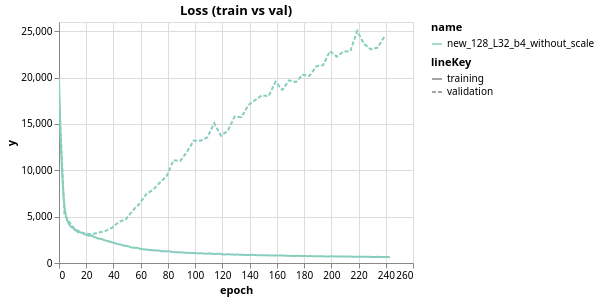
\includegraphics[width=\textwidth]{figures/vae_training_curves.png}  % uncomment with your file
  \fbox{\parbox[c][4cm][c]{0.9\textwidth}{\centering [Training and validation loss curves]}}
  \caption{Training and validation losses of the VAE. The validation loss does not follow
           the decrease of the training loss, indicating overfitting.}
  \label{fig:vae_curves}                 % referenced as Figure~\ref{fig:vae_curves}
\end{figure}

\begin{figure}[htbp]                     % placeholder for reconstruction examples
  \centering                             % center the figure
  % 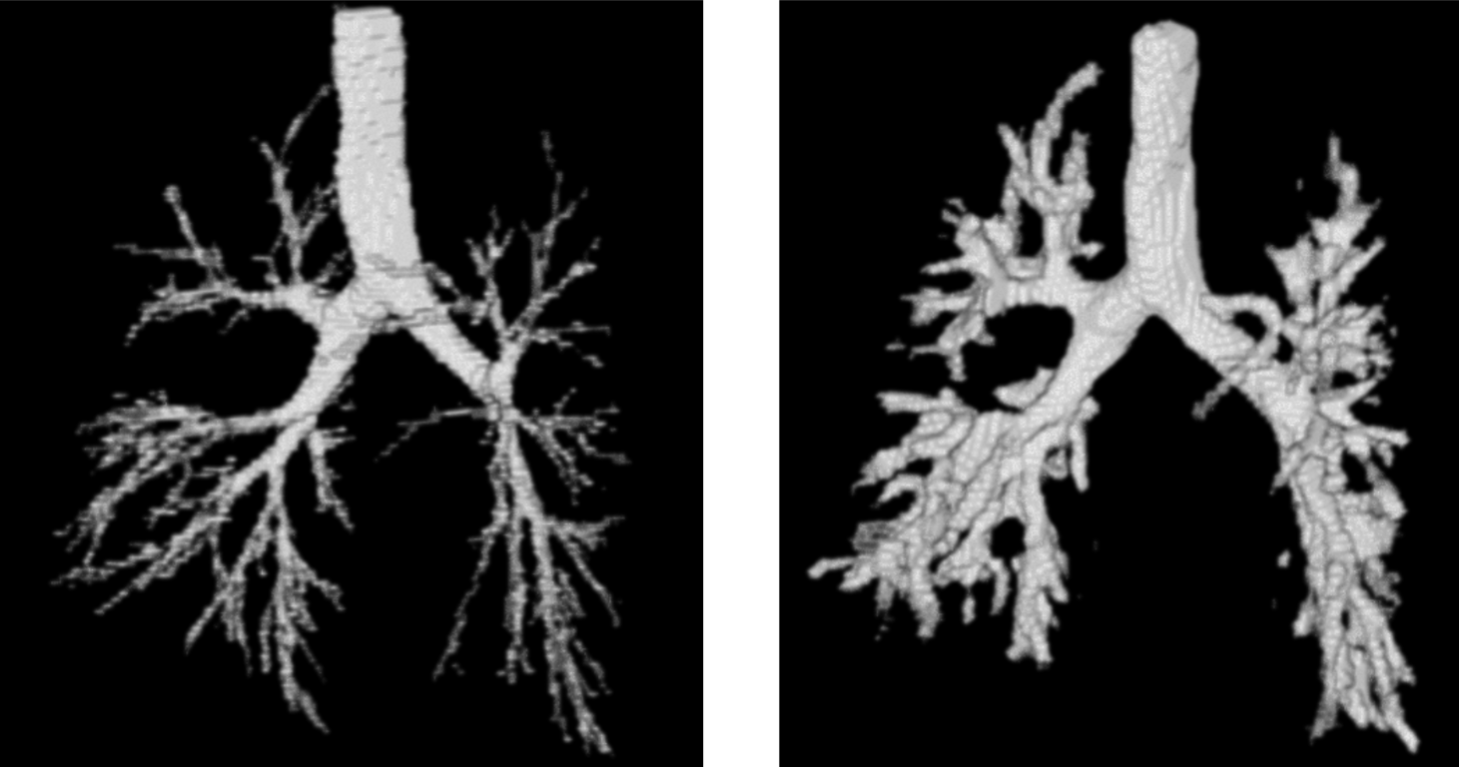
\includegraphics[width=\textwidth]{figures/vae_reconstructions.png}  % uncomment with your file
  \fbox{\parbox[c][4cm][c]{0.9\textwidth}{\centering [Original vs.\ reconstructed airway trees]}}
  \caption{Original airway trees and their VAE reconstructions for training (top) and
           validation/test (bottom) samples.}
  \label{fig:vae_recon}                  % referenced as Figure~\ref{fig:vae_recon}
\end{figure}

% ------------------------------------------------------------------------------
\subsubsection{Mitigating overfitting}   % augmentation and dropout attempts
\label{sec:vae_overfitting}              % \secref{sec:vae_overfitting}

To reduce overfitting, we applied two regularization strategies.

\paragraph{Data augmentation.}           % first regularization strategy
Each training sample was randomly transformed with \TODO{random translations, flips,
rotations, small elastic deformations, noise}. This increases the effective size and
variability of the training set. \citet{brock2016} use a similar strategy, training on both a
corrupted and an uncorrupted copy of each instance so that the network learns invariance to
small structural variations.

\paragraph{Dropout.}                     % second regularization strategy
Dropout layers with rate \TODO{$p$} were added to \TODO{the fully connected layers / the
encoder / the decoder} to discourage co-adaptation of features.

Neither strategy resolved the problem. As shown in Figure~\ref{fig:vae_curves_reg}, the
training and validation curves still diverge after adding augmentation and dropout, and
validation and test reconstructions remain poor. This suggests the limitation lies deeper than
a lack of regularization. Plausible causes include the small size of the dataset relative to
model capacity, the low voxel resolution relative to the thinness of the airway branches, and
the difficulty voxel VAEs have with thin structures.

\begin{figure}[htbp]                     % placeholder for curves after regularization
  \centering                             % center the figure
  % \includegraphics[width=\textwidth]{figures/vae_curves_regularized.png}  % uncomment with your file
  \fbox{\parbox[c][4cm][c]{0.9\textwidth}{\centering [Loss curves with augmentation and dropout]}}
  \caption{Training and validation losses after adding data augmentation and dropout. The
           gap between training and validation performance persists.}
  \label{fig:vae_curves_reg}             % referenced as Figure~\ref{fig:vae_curves_reg}
\end{figure}
           % Subsection "Variational autoencoder"
% Deterministic and sparse autoencoders -- subsection of "Encoding",
% pulled in by sections/05-encoding.tex.

\subsection[Deterministic and sparse autoencoders]{Deterministic and Sparse Autoencoders}
\label{sec:ae}                           % \secref{sec:ae}

In addition to the VAEs described in \secref{sec:vae}, we trained two further variants at
both input resolutions ($128^3$ and $256^3$): a deterministic autoencoder, and a model with a
sparse convolutional encoder.

% ------------------------------------------------------------------------------
\subsubsection{Deterministic autoencoder}  % VAE with the variational part removed
\label{sec:ae_det}                       % \secref{sec:ae_det}

The deterministic autoencoder uses the same encoder and decoder as the VAE
(\secref{sec:vae_architecture}), with the variational part removed. Instead of two linear
layers predicting $\boldsymbol{\mu}$ and $\log\boldsymbol{\sigma}$, a single linear layer maps
the flattened encoder features directly to a latent code $\mathbf{z}$ of dimension
\TODO{100}. No sampling takes place, and the KL divergence term is dropped from the loss, so
the objective reduces to the weighted BCE, the clDice term and L2 weight regularization:
\begin{equation}
  \mathcal{L}_{\mathrm{AE}} = \mathcal{L}_{\mathrm{BCE\text{-}mod}}
  + \lambda\,(1 - \mathrm{clDice})
  + \mathcal{L}_{\mathrm{L2}}.
  \label{eq:ae_loss}                     % autoencoder loss without the KL term
\end{equation}
Without the KL term, the latent space is no longer pushed towards a unit Gaussian prior.
This means the model cannot be used to generate new trees by sampling, but the latent code
can still serve as a learned representation of each airway tree. Removing the KL term also
removes the trade-off between reconstruction quality and latent regularization. This lets us
test whether the KL term was responsible for the poor reconstructions of the VAE.

% ------------------------------------------------------------------------------
\subsubsection{Sparse encoder}           % encoder built on sparse voxel operators (XCube)
\label{sec:ae_sparse}                    % \secref{sec:ae_sparse}

\paragraph{Motivation.}                  % why sparsity suits airway trees
The second variant replaces the dense convolutional encoder with a sparse one, following
the sparse structure VAE of XCube \cite{ren2024}. Ren et al.\ argue that voxel grids are
flexible, can represent both bulky and thin structures, and allow fast querying and
processing. Sparse voxel representations go further by not storing any information for empty
regions, which makes them considerably more efficient \cite{ren2024}. This is particularly
relevant for airway trees: only a very small fraction of the $128^3$ or $256^3$ grid is
occupied, so a dense encoder spends most of its computation and memory on empty space.

\paragraph{Encoder design.}              % sparse conv + max pooling, as in XCube
As in XCube \cite{ren2024}, the encoder is built from neural network operators defined over
sparse voxel grids. It processes the input occupancy grid with a sparse convolutional neural
network that alternates between sparse convolutions and max pooling operations, reducing the
resolution step by step until it reaches the resolution of the latent representation. XCube
implements these operators on top of the VDB data structure \cite{museth2013}, whose compact
storage and fast look-up make sparse convolution and pooling efficient on the GPU. We
implemented the sparse encoder with \TODO{sparse convolution library, e.g.\ fVDB /
MinkowskiEngine / spconv}, using \TODO{number} sparse convolution layers and \TODO{number}
max pooling layers. The resulting sparse features are then \TODO{converted to a dense $7^3$
grid / globally pooled} and mapped to the latent code in the same way as in the dense model.

\paragraph{Decoder.}                     % decoder deliberately kept unchanged
We kept the decoder unchanged: it is the same dense decoder described in
\secref{sec:vae_architecture}. Note that XCube pairs its sparse encoder with a
structure-prediction decoder, which starts from the latent grid and progressively subdivides
existing voxels and prunes unnecessary ones until it reaches the output
resolution \cite{ren2024}. We did not adopt this decoder, so that any change in performance
could be attributed to the encoder alone. The sparse-encoder model was trained with the
\TODO{VAE objective of \secref{sec:vae_loss} / autoencoder objective of
Equation~\eqref{eq:ae_loss}}.

% ------------------------------------------------------------------------------
\subsubsection{Results}                  % same failure modes as the VAE
\label{sec:ae_results}                   % \secref{sec:ae_results}

Neither architecture produced satisfactory reconstructions. As with the VAE, reconstructions
of validation and test airway trees show \TODO{e.g.\ missing branches, broken connectivity,
blob-like structures} (Figure~\ref{fig:ae_recon}).

Both models also show the same overfitting behaviour as the VAE. The training loss decreases
steadily, while the validation loss does not follow it (Figure~\ref{fig:ae_curves}).
\TODO{Data augmentation and dropout were also applied to these models, without improvement.}

The deterministic autoencoder, the sparse-encoder model and the VAE all show the same
pattern. This suggests that the problem is not caused by the variational formulation or by
the type of encoder. More likely causes are the limited amount of training data relative to
model capacity and the difficulty of reconstructing thin, branching structures with a dense
voxel decoder.

\begin{figure}[htbp]                     % placeholder for AE and sparse reconstructions
  \centering                             % center the figure
  % 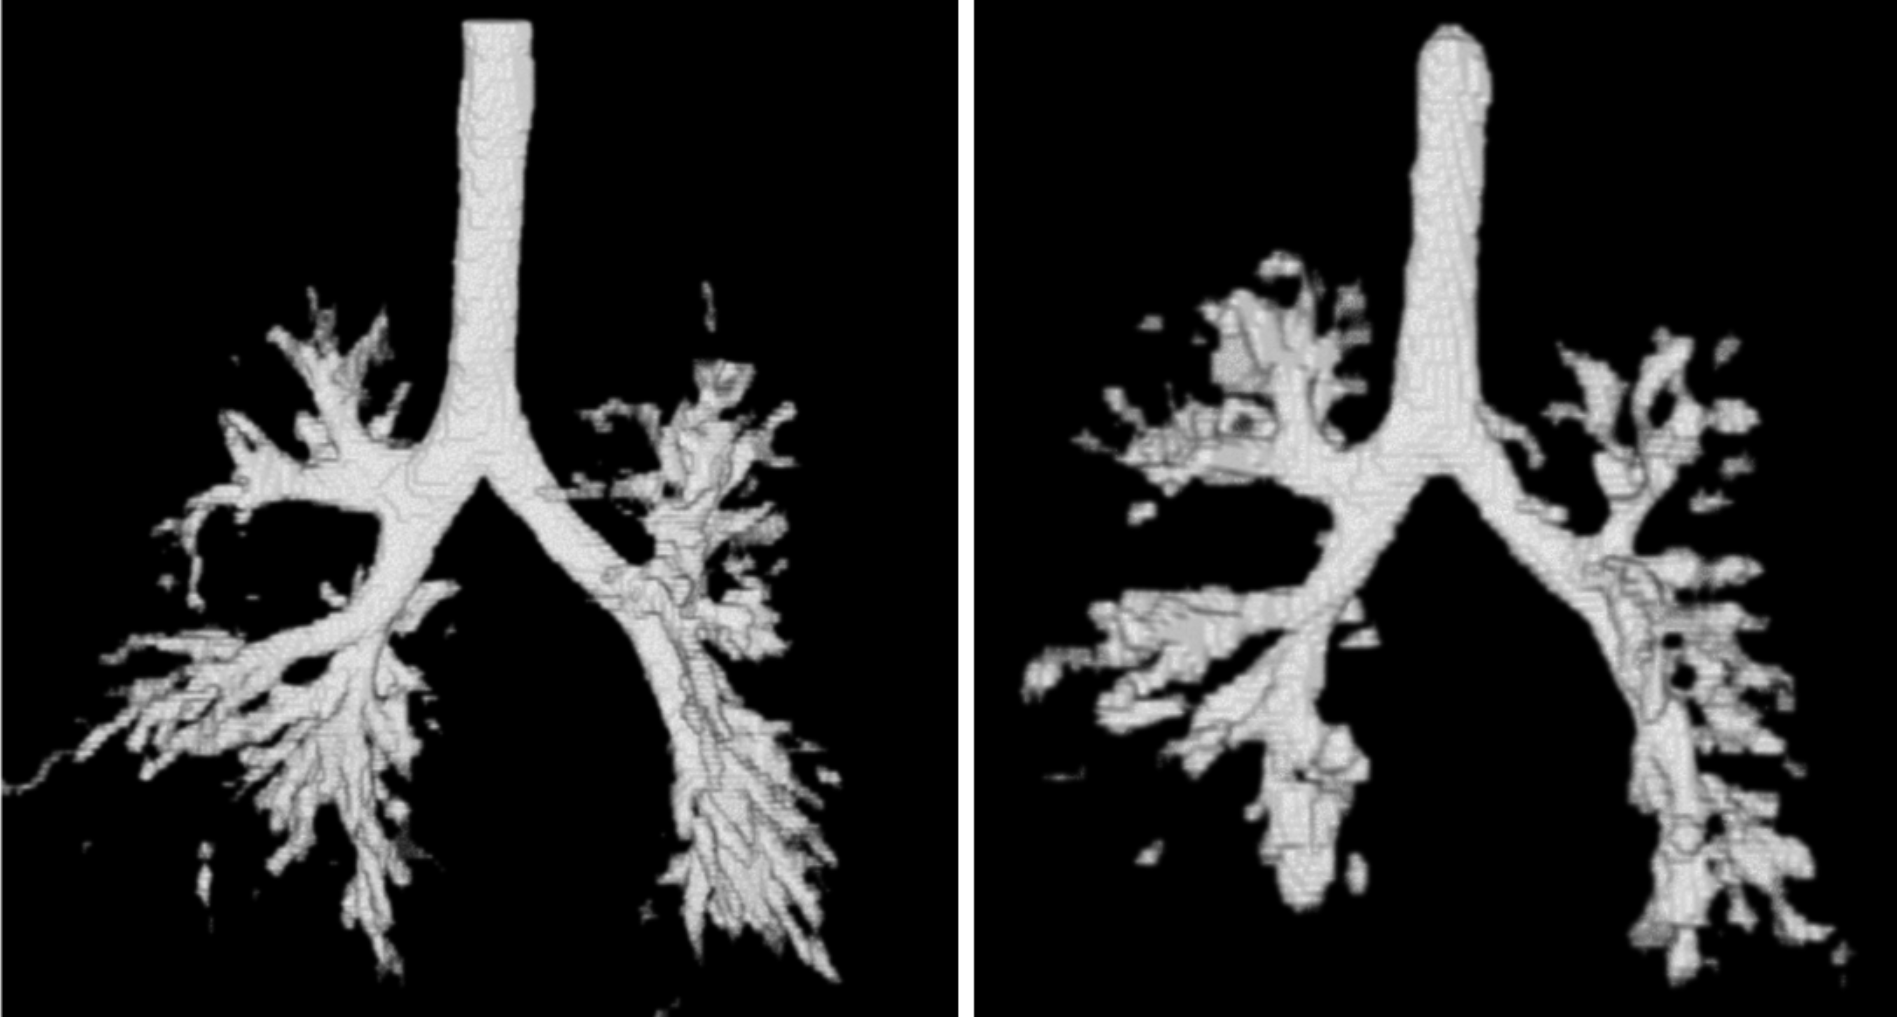
\includegraphics[width=\textwidth]{figures/ae_sparse_reconstructions.png}  % uncomment with your file
  \fbox{\parbox[c][4cm][c]{0.9\textwidth}{\centering [Reconstructions: autoencoder and sparse encoder]}}
  \caption{Original airway trees and their reconstructions from (a) the deterministic
           autoencoder and (b) the sparse-encoder model, for training and validation/test
           samples.}
  \label{fig:ae_recon}                   % referenced as Figure~\ref{fig:ae_recon}
\end{figure}

\begin{figure}[htbp]                     % placeholder for AE and sparse loss curves
  \centering                             % center the figure
  % \includegraphics[width=\textwidth]{figures/ae_sparse_curves.png}  % uncomment with your file
  \fbox{\parbox[c][4cm][c]{0.9\textwidth}{\centering [Loss curves: autoencoder and sparse encoder]}}
  \caption{Training and validation losses of (a) the deterministic autoencoder and (b) the
           sparse-encoder model. As with the VAE, the validation loss does not follow the
           training loss.}
  \label{fig:ae_curves}                  % referenced as Figure~\ref{fig:ae_curves}
\end{figure}
  % Subsection "Deterministic and sparse autoencoders"
% Implicit encoding (DeepSDF + DGCI SDF loss) -- subsection of "Encoding",
% pulled in by sections/05-encoding.tex.
% Red \TODO{...} marks replace the [square-bracket] placeholders of the original draft.
%
% ==============================================================================
% REVISION NOTES
% ------------------------------------------------------------------------------
% Rewritten to match the code in Airway_Tree/DeepSDF: the model is the original
% DeepSDF auto-decoder (Park et al. 2019), trained with the SDF loss of DGCI
% (Zhang et al. 2024, Eqs. 3-4) instead of DeepSDF's clamped L1. Removed: shared
% code beta, hypernetworks, encoder-decoder, correspondence loss, intra/inter
% regularization. All values below were read from examples/airways_new/specs.json,
% train_deep_sdf.py, deep_sdf/dgci_loss.py, networks/deep_sdf_decoder.py,
% reconstruct.py and Dgci/normalized_SDF_points/run_batch.sh.
%
% Notation: the instance code is now z_i (DeepSDF's symbol) instead of alpha_i.
% If the clustering section refers to alpha_i, rename it there too.
% Old \label names (sec:dgci*, fig:dgci*, tab:dgci*) are kept as aliases
% so existing \secref / \ref calls elsewhere keep working. Equation labels are renamed
% eq:dgci_* -> eq:implicit_* (amsmath allows only one \label per equation).
% ==============================================================================

\subsection[Implicit encoding]{Implicit Neural Representation of Airway Trees}
\label{sec:implicit}                     % \secref{sec:implicit}
\label{sec:dgci}                         % old name, kept so existing references still work

The voxel-based models of \secref{sec:vae} and \secref{sec:ae} did not produce
satisfactory reconstructions. We therefore trained an implicit model: the DeepSDF
auto-decoder of \citet{park2019}, optimized with the signed distance loss proposed for
airway trees by \citet{zhang2024} instead of the original DeepSDF loss. This model gave the
best reconstructions of all the architectures we tested, and its learned latent codes are
the representation used for the clustering in \secref{sec:clustering}.

% ------------------------------------------------------------------------------
\subsubsection{Motivation}               % why an implicit representation
\label{sec:implicit_motivation}          % \secref{sec:implicit_motivation}
\label{sec:dgci_motivation}              % old name

Airway annotations are made slice by slice in CT image stacks, so the reconstructed shape is
inevitably limited by the resolution of the discrete voxels, and the image contrast degrades
as the bronchi become thinner. As a result, voxel-based airway trees tend to be coarse and
affected by spike-like noise, and CNN-based methods, which also work in the discrete voxel
space, suffer from the same problems as well as from breakages in the tree \cite{zhang2024}.

Implicit neural representations (INRs) address this by using coordinate-based neural
networks to parameterize a shape in continuous physical space instead of on a voxel grid.
They are therefore not bounded by the CT grid resolution, and they yield smoother shapes
with fewer spike-like artifacts \cite{park2019,zhang2024}. DeepSDF \cite{park2019} learns a
single network that represents a whole class of shapes, each shape being identified by a
low-dimensional latent code. These codes form a compact, continuous embedding of the
training shapes, which is what we need for clustering.

However, \citet{zhang2024} observed that the loss used by DeepSDF, an L1 penalty on the
predicted SDF values, is not sufficient to model fine airway structures with high fidelity.
They proposed additional geometric constraints, derived from implicit geometric
regularization \cite{gropp2020}, as part of their Deep Geometric Correspondence Implicit
(DGCI) model. We kept the DeepSDF architecture and adopted only this loss
(\secref{sec:implicit_loss}).
% [NOTE] If you also trained the full DGCI model (jobs/job_train_DGCI.sh) and it did worse,
% say so here in one sentence -- it justifies the choice of plain DeepSDF.

% ------------------------------------------------------------------------------
\subsubsection{Model}                    % auto-decoder + network
\label{sec:implicit_architecture}        % \secref{sec:implicit_architecture}
\label{sec:dgci_architecture}            % old name

\paragraph{Neural signed distance field.}  % the implicit function F
Each airway tree is represented by its signed distance function (SDF), which gives, for any
point in space, the distance to the closest point of the airway surface, with a negative
sign inside the lumen and a positive sign outside \cite{park2019}. A single neural network
$f_\theta$ represents the SDFs of all trees. It takes a coordinate
$\mathbf{p} \in \mathbb{R}^3$ together with a latent code $\mathbf{z}_i \in \mathbb{R}^K$
specific to the $i$-th airway tree, and predicts the signed distance of $\mathbf{p}$ to the
surface of that tree:
\begin{equation}
  \mathcal{F}(\mathbf{p}; \mathbf{z}_i) = f_\theta(\mathbf{z}_i, \mathbf{p})
  \approx \mathrm{SDF}_i(\mathbf{p}),
  \qquad f_\theta : \mathbb{R}^{K+3} \to \mathbb{R}.
  \label{eq:implicit_sdf}                % the neural SDF mapping
\end{equation}
The airway surface of tree $i$ is the zero level set of $\mathcal{F}(\cdot\,; \mathbf{z}_i)$,
and can be extracted as a mesh with Marching Cubes \cite{lorensen1987}.

\paragraph{Auto-decoder.}                % no encoder, codes are free parameters
DeepSDF has no encoder (Figure~\ref{fig:implicit_arch}). Instead, each training tree is
assigned a latent code $\mathbf{z}_i$ that is a free parameter, randomly initialized and
optimized jointly with the network weights $\theta$ by backpropagation
\cite{park2019}. After training, the decoder weights are fixed, and the code of a new tree
is obtained by optimizing $\mathbf{z}$ alone so that $\mathcal{F}(\cdot\,; \mathbf{z})$ fits
the samples of that tree (\secref{sec:implicit_inference}).

\paragraph{Network.}                     % layer sizes, skip connection
Following \citet{park2019}, $f_\theta$ is a multilayer perceptron with eight hidden
fully connected layers of 512 units, each with weight normalization \cite{salimans2016} and
no dropout. The input is the concatenation $[\mathbf{z}_i, \mathbf{p}]$, and the same vector
is concatenated again to the output of the fourth layer (skip connection). We use latent
codes of dimension $K = 256$.

\paragraph{Changes required by the geometric loss.}  % IGR-style modifications
The loss of \secref{sec:implicit_loss} constrains the spatial gradient
$\nabla_{\mathbf{p}}\mathcal{F}$, so training backpropagates through this gradient. We
therefore made three changes to the original DeepSDF network, following implicit geometric
regularization \cite{gropp2020}:
\begin{itemize}                          % the three architectural changes
  \item the ReLU activations are replaced by Softplus with $\beta = 100$, a smooth
        approximation of ReLU whose gradient is continuous, so that the gradient terms of
        the loss can themselves be differentiated;
  \item the final $\tanh$ is removed, because it bounds $|\mathcal{F}| < 1$ and flattens the
        output far from the surface, which conflicts with the unit-gradient (Eikonal)
        constraint;
  \item the weights are initialized with the geometric initialization of
        \citet{gropp2020}, so that before training the network approximates the SDF of a
        sphere of radius 0.5. The weights reading the latent code start at zero, so every
        tree starts from the same sphere.
\end{itemize}

\begin{figure}[htbp]                     % placeholder for the architecture diagram
  \centering                             % center the figure
  % 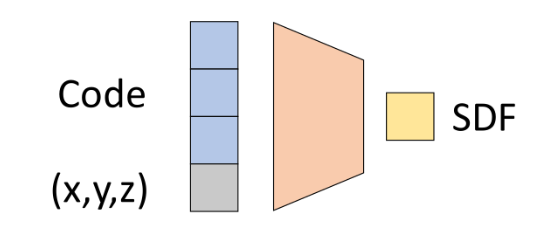
\includegraphics[width=\textwidth]{figures/deepsdf_architecture.png}  % uncomment with your file
  \fbox{\parbox[c][4cm][c]{0.9\textwidth}{\centering [DeepSDF auto-decoder figure]}}  % remove once image added
  \caption{The DeepSDF auto-decoder, adapted from \citet{park2019}. The latent code
           $\mathbf{z}_i \in \mathbb{R}^{256}$ of tree $i$ is concatenated with a query point
           $\mathbf{p}$ and passed through eight fully connected layers of width 512, with the
           input concatenated again after the fourth layer, to predict the signed distance
           $\mathcal{F}(\mathbf{p}; \mathbf{z}_i)$. The codes have no encoder: they are
           optimized together with the network weights.}
  \label{fig:implicit_arch}              % referenced as Figure~\ref{fig:implicit_arch}
  \label{fig:dgci_arch}                  % old name
\end{figure}

% ------------------------------------------------------------------------------
\subsubsection{Loss function}            % DGCI SDF loss + DeepSDF code regularization
\label{sec:implicit_loss}                % \secref{sec:implicit_loss}
\label{sec:dgci_loss}                    % old name



\paragraph{Sample sets.}                 % the three kinds of points per tree
For each tree $i$ of a mini-batch $\mathcal{B}$, three sets of points are drawn in every
iteration (\secref{sec:implicit_training}): surface points $S_i$, with their ground-truth
outward normals $\mathbf{n}'$; free-space points $V_i$ near and away from the surface, with
their ground-truth signed distances $s'$; and points $U_i$ drawn uniformly in the normalized
volume $[-1,1]^3$, which have no ground truth. On the surface, $s' = 0$. We write
$\Omega_i = S_i \cup V_i \cup U_i$ for all points of tree $i$, and, for a family of sets
$A_i$, $|A| = \sum_{i \in \mathcal{B}} |A_i|$ for its total number of points in the
mini-batch.

\paragraph{SDF loss.}                    % Eqs. 3-4 of Zhang et al. without beta
We use the SDF loss of \citet{zhang2024}, written here without their shared code, so that
$\mathcal{F}$ depends only on $\mathbf{z}_i$. It has two parts,
$\mathcal{L}_{\mathrm{sdf}} = \mathcal{L}_{\mathrm{sdf\text{-}val}} +
\mathcal{L}_{\mathrm{sdf\text{-}geo}}$, which supervise the values and the geometry of the
predicted SDF respectively:
\begin{equation}
  \mathcal{L}_{\mathrm{sdf\text{-}val}} =
  \frac{\omega_s}{|S \cup V|} \sum_{i \in \mathcal{B}} \sum_{\mathbf{p} \in S_i \cup V_i}
      \big|\mathcal{F}(\mathbf{p}; \mathbf{z}_i) - s'\big|
  + \frac{\omega_\varphi}{|U|} \sum_{i \in \mathcal{B}} \sum_{\mathbf{p} \in U_i}
      \varphi\big(\mathcal{F}(\mathbf{p}; \mathbf{z}_i)\big),
  \label{eq:implicit_val}                % SDF value term
\end{equation}
\begin{equation}
  \begin{split}
    \mathcal{L}_{\mathrm{sdf\text{-}geo}} =
    &\frac{\omega_n}{|S|} \sum_{i \in \mathcal{B}} \sum_{\mathbf{p} \in S_i}
        \big(1 - S_{\cos}(\nabla\mathcal{F}(\mathbf{p}; \mathbf{z}_i), \mathbf{n}')\big) \\
    &+ \frac{\omega_{\mathrm{Eik}}}{|\Omega|} \sum_{i \in \mathcal{B}} \sum_{\mathbf{p} \in \Omega_i}
        \big|\,\|\nabla\mathcal{F}(\mathbf{p}; \mathbf{z}_i)\|_2 - 1\big|,
  \end{split}
  \label{eq:implicit_geo}                % normal consistency + Eikonal term (split to fit)
\end{equation}
where $S_{\cos}$ is the cosine similarity and the gradient is taken with respect to
$\mathbf{p}$. Unlike \citet{zhang2024}, who sum over the points, we divide each term by the
number of points of its set in the mini-batch, so every term is a mean and the weights do
not depend on the number of samples.


% \paragraph{Sample sets.}                 % the three kinds of points per tree
% For each tree $i$, three sets of points are drawn in every iteration
% (\secref{sec:implicit_training}): surface points $S_i$, with their ground-truth outward
% normals $\mathbf{n}'$; free-space points $V_i$ near and away from the surface, with their
% ground-truth signed distances $s'$; and points $U_i$ drawn uniformly in the normalized
% volume $[-1,1]^3$, which have no ground truth. On the surface, $s' = 0$.

% \paragraph{SDF loss.}                    % Eqs. 3-4 of Zhang et al. without beta
% We use the SDF loss of \citet{zhang2024}, written here without their shared code, so that
% $\mathcal{F}$ depends only on $\mathbf{z}_i$. It has two parts,
% $\mathcal{L}_{\mathrm{sdf}} = \mathcal{L}_{\mathrm{sdf\text{-}val}} +
% \mathcal{L}_{\mathrm{sdf\text{-}geo}}$, which supervise the values and the geometry of the
% predicted SDF respectively:
% \begin{equation}
%   \mathcal{L}_{\mathrm{sdf\text{-}val}} = \sum_i \Big(
%   \omega_s \sum_{\mathbf{p} \in S_i \cup V_i}
%       \big|\mathcal{F}(\mathbf{p}; \mathbf{z}_i) - s'\big|
%   + \omega_\varphi \sum_{\mathbf{p} \in U_i}
%       \varphi\big(\mathcal{F}(\mathbf{p}; \mathbf{z}_i)\big)
%   \Big),
%   \label{eq:implicit_val}                % SDF value term
% \end{equation}
% \begin{equation}
%   \begin{split}
%     \mathcal{L}_{\mathrm{sdf\text{-}geo}} = \sum_i \Big(
%     &\omega_n \sum_{\mathbf{p} \in S_i}
%         \big(1 - S_{\cos}(\nabla\mathcal{F}(\mathbf{p}; \mathbf{z}_i), \mathbf{n}')\big) \\
%     &+ \omega_{\mathrm{Eik}} \sum_{\mathbf{p} \in S_i \cup V_i \cup U_i}
%         \big|\,\|\nabla\mathcal{F}(\mathbf{p}; \mathbf{z}_i)\|_2 - 1\big|
%     \Big),
%   \end{split}
%   \label{eq:implicit_geo}                % normal consistency + Eikonal term (split to fit)
% \end{equation}




% where $S_{\cos}$ is the cosine similarity and the gradient is taken with respect to
% $\mathbf{p}$. In practice, each sum is normalized by the number of points of its set in the
% mini-batch, so every term is a mean and the weights do not depend on the number of samples.

The first term of Equation~\eqref{eq:implicit_val} regresses the SDF values directly. Unlike
DeepSDF, which clamps both prediction and target to $[-0.1, 0.1]$ \cite{park2019}, it is
applied without clamping. The second term, with $\varphi(s) = \exp(-\delta |s|)$ and
$\delta = 100$, penalizes points away from the surface whose predicted SDF is close to zero,
and therefore suppresses spurious surfaces in empty space \cite{zhang2024}. \citet{zhang2024}
write this term over all off-surface points; we apply it, as in their released code, only to
the uniform points $U_i$, because many free-space points $V_i$ lie very close to the surface,
where a small SDF is correct and should not be penalized. Equation~\eqref{eq:implicit_geo}
aligns the SDF gradient with the surface normals and constrains its norm to one everywhere,
as required for a true distance function (Eikonal equation) \cite{gropp2020,zhang2024}.

\paragraph{Latent code regularization.}  % DeepSDF's prior on the codes
\citet{zhang2024} regularize their instance and shared codes and add a correspondence loss
for their encoder--decoder. Since our model has neither a shared code nor an
encoder--decoder, we keep instead the code regularization of the DeepSDF implementation,
which corresponds to a zero-mean Gaussian prior on the codes \cite{park2019}:
\begin{equation}
  \mathcal{L}_{\mathrm{reg}} = \lambda \, \min\!\Big(1, \frac{t}{100}\Big)
      \frac{1}{B} \sum_{i \in \mathcal{B}} \|\mathbf{z}_i\|_2,
  \label{eq:implicit_reg}                % code regularization with warm-up
\end{equation}
where $\mathcal{B}$ is the mini-batch of $B$ trees, $t$ the epoch, and $\lambda = 0.3$. The
factor $\min(1, t/100)$ increases the regularization linearly over the first 100 epochs. In
addition, the norm of every code is capped at 1.

\paragraph{Total objective.}             % what is minimized
The decoder weights $\theta$ and all training codes $\{\mathbf{z}_i\}$ are optimized jointly
by minimizing
\begin{equation}
  \mathcal{L}_{\mathrm{total}} = \mathcal{L}_{\mathrm{sdf\text{-}val}}
  + \mathcal{L}_{\mathrm{sdf\text{-}geo}} + \mathcal{L}_{\mathrm{reg}}.
  \label{eq:implicit_total}              % full training loss
\end{equation}
Following \citet{zhang2024}, we set $\omega_s = 3\times10^3$,
$\omega_\varphi = 5\times10^2$, $\omega_n = 10^2$ and $\omega_{\mathrm{Eik}} = 5\times10^1$.

% ------------------------------------------------------------------------------
\subsubsection{Data preparation and training}  % SDF sampling, optimizer, schedule
\label{sec:implicit_training}            % \secref{sec:implicit_training}
\label{sec:dgci_training}                % old name

\paragraph{Data.}                        % meshes, normalization, samples
Our dataset contains \TODO{N} airway trees from the AIIB23 \TODO{\cite{...}} and ATM22
\TODO{\cite{...}} datasets, split into \TODO{$N_{\mathrm{train}}$} training,
\TODO{$N_{\mathrm{val}}$} validation and \TODO{$N_{\mathrm{test}}$} test cases. Each airway
surface was extracted from its binary segmentation with Marching
Cubes \cite{lorensen1987}, and the SDF samples were prepared with the preprocessing of
DeepSDF \cite{park2019}. Each mesh is centered on its bounding box and scaled to fit in the
unit sphere with a margin of 3\%; the offset and scale are stored, so that predictions can
be mapped back to CT coordinates. Then, for each tree:
\begin{itemize}                          % the two sample files per tree
  \item 200,000 surface points with outward normals are obtained by rendering the mesh
        from virtual cameras placed around it and back-projecting the depth maps;
  \item 500,000 SDF samples are generated: 94\% near the surface, by perturbing surface
        points with Gaussian noise of variance $5\times10^{-4}$ and $5\times10^{-5}$, and
        6\% uniformly in $[-1,1]^3$. Their signed distance is the distance to the closest
        surface point, with the sign given by the orientation of the closest normals.
\end{itemize}
% [NOTE] Marching Cubes / mask-to-mesh step: confirm it is the one in jobs/job_nifti_to_mesh.sh.

\paragraph{Training.}                    % sampling per iteration, optimizer, schedule
In every iteration, we draw for each tree 4,096 surface points ($S_i$), 4,096 free-space
points ($V_i$), half of them inside and half outside the airway, and 2,048 uniform points
($U_i$). Balancing inside and outside samples is important for airways, since the lumen
occupies only a small fraction of the normalized volume and most samples are naturally
outside. The mini-batch contains $B = 64$ trees. The decoder weights and the latent codes
are optimized with Adam \cite{kingma2015}, with initial learning rates of $10^{-3}$ and
$2\times10^{-3}$ respectively, both halved every 4,000 epochs. The codes are initialized
from $\mathcal{N}(0, 1/K)$. The model was trained for \TODO{E} epochs on a single
\TODO{NVIDIA A100 / L40S} GPU. The training losses are shown in
Figure~\ref{fig:implicit_curves}.
% [NOTE] specs.json allows 20,001 epochs; report the epoch of the checkpoint you actually used.

After training, each training tree is represented by its latent code
$\mathbf{z}_i \in \mathbb{R}^{256}$. These codes are the features used for clustering in
\secref{sec:clustering}.

\paragraph{Latent codes of unseen trees.}  % test-time optimization
\label{sec:implicit_inference}           % \secref{sec:implicit_inference}
For validation and test trees, the decoder weights are frozen and only a new code
$\mathbf{z}$ is optimized \cite{park2019}. The code is initialized from
$\mathcal{N}(0, 0.01^2)$ and optimized for 800 iterations with Adam, with a learning rate of
$5\times10^{-3}$ divided by 10 after 400 iterations. The objective is the same SDF loss,
$\mathcal{L}_{\mathrm{sdf\text{-}val}} + \mathcal{L}_{\mathrm{sdf\text{-}geo}}$, on freshly
drawn samples of the tree, plus a prior term
$10^{-4}\,\omega_s \,\overline{\mathbf{z}^2}$, where $\overline{\mathbf{z}^2}$ is the mean of
the squared code entries.
% [NOTE] if the clustering uses only training codes, this paragraph is only needed for
% the validation/test reconstruction metrics below.

\begin{figure}[htbp]                     % placeholder for training curves
  \centering                             % center the figure
  % \includegraphics[width=\textwidth]{figures/deepsdf_training_curves.png}  % uncomment with your file
  \fbox{\parbox[c][4cm][c]{0.9\textwidth}{\centering [DeepSDF training loss curves]}}  % remove once image added
  \caption{Training losses of the DeepSDF model: total loss and the weighted terms of
           Equations~\eqref{eq:implicit_val}--\eqref{eq:implicit_reg} (SDF value, $\varphi$,
           normal, Eikonal and code regularization).}
  \label{fig:implicit_curves}            % referenced as Figure~\ref{fig:implicit_curves}
  \label{fig:dgci_curves}                % old name
\end{figure}
% [NOTE] the auto-decoder has no validation loss during training (validation codes are only
% fitted afterwards), so the old "training and validation losses" wording was removed.
% train_deep_sdf.py logs the per-term values each epoch; plot_log.py plots them.

% ------------------------------------------------------------------------------
\subsubsection{Evaluation metrics}       % continuous-space and voxel-space metrics
\label{sec:implicit_metrics}             % \secref{sec:implicit_metrics}
\label{sec:dgci_metrics}                 % old name

We follow the evaluation protocol of \citet{zhang2024}, which measures shape quality both in
continuous space, on the mesh extracted from the predicted SDF, and in discrete voxel space.
Meshes are extracted with Marching Cubes on a $\TODO{256}^3$ grid in the normalized volume.

\paragraph{Continuous space.}            % non-manifold counts on the mesh
Smoothness and connectivity of the reconstructed mesh are measured by counting non-manifold
(NM) elements. NM-V counts the vertices connected to three or more non-coplanar faces, NM-E
counts the edges shared by three or more faces, and NM-F counts the faces arranged in a way
that prevents a closed, continuous body from being formed. Fewer non-manifold elements
indicate better connectivity and smoothness \cite{zhang2024}.

\paragraph{Discrete space.}              % topology metrics on the voxelized result
To compute voxel-based metrics, the predicted SDF is evaluated directly on the voxel grid of
the original CT image: the center of each voxel is mapped to the normalized volume with the
stored offset and scale, and the voxel is labeled as airway if the predicted SDF is negative
\TODO{(with $2\times$ supersampling near the surface and a 50\% occupancy threshold)}. On this
volume we compute the tree length detected rate (TD) and the branch detected rate (BD),
defined in Eq.~\eqref{eq:td_bd}, and the Dice coefficient, which measure the topological
completeness and correctness of the reconstruction \cite{zhang2024}.
% [NOTE] this describes track_reconstruction.voxelize (same procedure as DGCI's create_mask).
% If your final evaluation used mesh voxelization + hole filling instead, revert to that.

% ------------------------------------------------------------------------------
\subsubsection{Results}                  % quantitative and qualitative results
\label{sec:implicit_results}             % \secref{sec:implicit_results}
\label{sec:dgci_results}                 % old name

Table~\ref{tab:implicit_results} reports the metrics on the \TODO{validation and test} sets,
and Figure~\ref{fig:implicit_recon} shows examples of reconstructed airway trees. This model
produced the best reconstructions of all the models we trained. \TODO{Describe the main
observations, e.g.\ preservation of fine distal branches, connectivity of the tree,
smoothness of the surface.}

\begin{table}[htbp]                      % quantitative results
  \centering                             % center the table
  \small                                 % slightly smaller font so the table fits
  \caption{Reconstruction results of the DeepSDF model trained with the SDF loss of
           \citet{zhang2024}, reported as mean $\pm$ standard deviation.}
  \label{tab:implicit_results}           % referenced as Table~\ref{tab:implicit_results}
  \label{tab:dgci_results}               % old name
  \begin{tabular}{lcccccc}               % set name + 6 metrics
    \toprule
    & \multicolumn{3}{c}{Continuous space} & \multicolumn{3}{c}{Discrete space} \\
    \cmidrule(lr){2-4} \cmidrule(lr){5-7}  % group underlines (lr = trim ends)
    Set & NM-V $\downarrow$ & NM-E $\downarrow$ & NM-F $\downarrow$
        & TD (\%) $\uparrow$ & BD (\%) $\uparrow$ & Dice (\%) $\uparrow$ \\
    \midrule
    Validation & \TODO{?} & \TODO{?} & \TODO{?} & \TODO{?} & \TODO{?} & \TODO{?} \\
    Test       & \TODO{?} & \TODO{?} & \TODO{?} & \TODO{?} & \TODO{?} & \TODO{?} \\
    \bottomrule
  \end{tabular}
\end{table}

\begin{figure}[htbp]                     % placeholder for reconstructions
  \centering                             % center the figure
  % \includegraphics[width=\textwidth]{figures/deepsdf_reconstructions.png}  % uncomment with your file
  \fbox{\parbox[c][4cm][c]{0.9\textwidth}{\centering [Original vs.\ reconstructed airway trees]}}  % remove once image added
  \caption{Ground-truth airway trees and their reconstructions by the DeepSDF model.}
  \label{fig:implicit_recon}             % referenced as Figure~\ref{fig:implicit_recon}
  \label{fig:dgci_recon}                 % old name
\end{figure}      % Subsection "Implicit encoding"

% Labelling -- anatomical labelling of the airway trees with the released IPGN model.
% Red \TODO{...} marks replace the [square-bracket] placeholders of the original draft.

\section[Labelling]{Anatomical Labeling of Airway Trees}
\label{sec:labeling}                     % \secref{sec:labeling}

To assign anatomical labels to our airway trees, we used the Implicit Point-Graph Network
(IPGN) of \citet{xie2025}. We did not train this model ourselves: we used the weights
released by the authors, trained on their Pulmonary Tree Labeling (PTL) dataset, and ran the
model in inference mode only. This section describes how the model is formulated and how it
was trained, so that its predictions on our data can be interpreted.

% ------------------------------------------------------------------------------
\subsection{Task formulation}            % 19-class labeling of a binary tree
\label{sec:labeling_task}                % \secref{sec:labeling_task}

The input to the model is a binary volume containing a pulmonary tree (airway, artery or
vein). The goal is a 19-class semantic segmentation of every foreground voxel: 18 classes
correspond to segmental-level branches, i.e.\ the branches that supply the 18 pulmonary
segments, and one class corresponds to the extra-pulmonary structures \cite{xie2025}. Labels
1 to 10 are branches in the left lung, labels 11 to 18 are branches in the right lung, and
label 19 is the extra-pulmonary part (for the airway, the trachea and main
bronchi) \cite{xie2025}.

Xie et al.\ point out that the hardest part of this task is labeling the branching points and
the distal end points correctly. These key locations contain very few voxels compared to the
rest of the tree, so a model trained only on voxel-wise signals is dominated by easy voxels
and can achieve a high voxel-level score while still mislabeling key
locations \cite{xie2025}. For this reason, IPGN also represents each tree as a skeleton graph
whose nodes approximate these key points, and it is evaluated on both voxels and graph
elements.

% ------------------------------------------------------------------------------
\subsection{Training data}               % PTL dataset and skeleton graph labels
\label{sec:labeling_data}                % \secref{sec:labeling_data}

\paragraph{PTL dataset.}                 % the data the released model was trained on
The model was trained on the PTL dataset, compiled by the authors from multiple medical
centers \cite{xie2025}. It contains 800 subjects, each with three volumes (airway, artery and
vein) annotated with the 19 classes above. All volumes have size $N \times 512 \times 512$,
with $N$ between 181 and 798 slices and a slice spacing between 0.5 and 1.5~mm. The
annotations were produced by a junior radiologist and verified by a senior radiologist.
During training, each annotated volume is converted to a binary input, and the original
labeled volume is the prediction target. The dataset was split randomly into 70\% training,
10\% validation and 20\% test subjects \cite{xie2025}.

\paragraph{Skeleton graphs.}             % how graphs are built from volumes
For each volume, a skeleton graph is built with the VesselVio software \cite{bumgarner2022},
which applies the thinning algorithm of \citet{lee1994} to extract the centerlines of the
tree. In the resulting graph, the centerline segments become edges representing anatomical
connections, and the centerline intersections and distal end points become nodes
representing the key points of the tree \cite{xie2025}. No additional hyperparameters or
modeling are involved: all spatial and connectivity information comes directly from the
original volume.

\paragraph{Graph labels.}                % three-step labeling procedure
Ground-truth labels for the graph are derived from the annotated volume in three steps,
labeling edges before nodes because edge labels are deterministic while node labels can be
ambiguous where classes meet \cite{xie2025}:
\begin{enumerate}                        % the graph labeling procedure
  \item \textbf{Graph simplification.} VesselVio also outputs, for each edge, the connected
        centerline points along it. Software inconsistencies can create cliques among
        these points; they are removed by keeping only the shortest path between the two
        nodes.
  \item \textbf{Edge labeling.} The labels of the centerline points of each edge are read
        from the annotated volume, and the edge label is their majority vote.
  \item \textbf{Node labeling.} A leaf node takes the label of its single edge, which is
        more reliable than reading it from the volume, since leaf coordinates can fall
        slightly outside the foreground. A node with several edges takes the majority vote
        of the labels of its connected edges.
\end{enumerate}

% ------------------------------------------------------------------------------
\subsection{Model architecture}          % PGN backbone + Implicit Point Module
\label{sec:labeling_architecture}        % \secref{sec:labeling_architecture}

\paragraph{Overview.}                    % the three stages of IPGN
Instead of processing the dense volume with a CNN, IPGN works on two sparse representations
of the tree: a point cloud, obtained by randomly sampling $M = 6{,}000$ foreground voxels,
and the skeleton graph with $N$ nodes \cite{xie2025}. The point cloud is a downsampled
version of the volume, while the graph describes the skeleton of the tree. The model has three
stages (Figure~\ref{fig:ipgn_overview}): separate point and graph encoders, a sequence of
Point-Graph Fusion layers that exchange information between the two branches, and an
Implicit Point Module that turns the sparse predictions back into a dense labeled volume. The
network without the implicit part is called the Point-Graph Network (PGN), and the full
model is IPGN \cite{xie2025}.

\paragraph{Notation.}                    % points, nodes and layer features
The point coordinates are $\mathbf{P} = \{\mathbf{p}_1, \dots, \mathbf{p}_M\} \in
\mathbb{R}^{M\times3}$ and the graph node coordinates are $\mathbf{G} = \{\mathbf{g}_1,
\dots, \mathbf{g}_N\} \in \mathbb{R}^{N\times3}$. A superscript $(i)$ denotes the feature of
an element after the $i$-th layer, e.g.\ $\mathbf{p}^{(i)}$ and $\mathbf{g}^{(i)}$, and
$\frown$ denotes concatenation \cite{xie2025}.

\paragraph{Point and graph encoders.}    % initial per-element features
The $(x, y, z)$ coordinates of the points and of the graph nodes are the only input features.
A point network and a graph network act as initial encoders and produce a 128-dimensional
feature for each point and each node, $\mathbf{P}^{(0)} \in \mathbb{R}^{M\times128}$ and
$\mathbf{G}^{(0)} \in \mathbb{R}^{N\times128}$ \cite{xie2025}. The point encoder is either
PointNet++ \cite{qi2017} or Point Transformer \cite{zhao2021}, and the graph encoder is an
11-layer graph attention network (GAT) \cite{velickovic2018} with 128 channels. The model we
used has a \TODO{PointNet++ / Point Transformer} point encoder.

\paragraph{Point-Graph Fusion layers.}   % two-way feature exchange
The core of the model is a stack of $l$ Point-Graph Fusion layers
(Figure~\ref{fig:ipgn_fusion}). Each layer takes $\mathbf{P}^{(i-1)}$ and
$\mathbf{G}^{(i-1)}$ and outputs $\mathbf{P}^{(i)}$ and $\mathbf{G}^{(i)}$, using the 3D
coordinates of the elements to find neighbors in the other branch \cite{xie2025}.

\emph{Point to graph (ball query and grouping).} Each graph node $\mathbf{g}$ collects all
points within a ball of radius $r$ around it, $\{\mathbf{p}_1, \dots, \mathbf{p}_b\}$, in
the style of PointNet++ \cite{qi2017}. An MLP $\mathcal{F}_1$ updates each of these point
features independently, and feature-wise max pooling aggregates them into a point summary
for the node \cite{xie2025}:
\begin{equation}
  \mathbf{g}^{(i)}_{bq} = \max_{j}\, \mathcal{F}_1\big(\mathbf{p}^{(i-1)}_j\big).
  \label{eq:ipgn_bq}                     % ball query + max pooling
\end{equation}
This summary is concatenated with the current node feature and passed through a shallow
graph attention network $\mathcal{G}$ \cite{velickovic2018}, which performs graph
convolution to produce the updated node feature:
\begin{equation}
  \mathbf{g}^{(i)} = \mathcal{G}\big(\mathbf{g}^{(i-1)} \frown \mathbf{g}^{(i)}_{bq}\big),
  \qquad \mathcal{G}: \mathbb{R}^{2D} \to \mathbb{R}^{D_{\mathrm{next}}}.
  \label{eq:ipgn_gat}                    % graph update with GAT
\end{equation}

\emph{Graph to point (feature propagation).} Each point $\mathbf{p}$ finds its $k$ nearest
graph nodes $\{\mathbf{g}_1, \dots, \mathbf{g}_k\}$ in coordinate space, at distances
$\{d_1, \dots, d_k\}$, and combines their features with weights given by the normalized
inverse distances \cite{rossi2021,xie2025}:
\begin{equation}
  \mathbf{p}^{(i)}_{fp} = \frac{\sum_{j=1}^{k} \mathbf{g}^{(i-1)}_j \cdot \frac{1}{d_j}}
                               {\sum_{l=1}^{k} \frac{1}{d_l}}.
  \label{eq:ipgn_fp}                     % inverse-distance feature propagation
\end{equation}
The result is concatenated with the incoming point feature, and an MLP $\mathcal{F}_2$
projects it to the next layer's dimension:
\begin{equation}
  \mathbf{p}^{(i)} = \mathcal{F}_2\big(\mathbf{p}^{(i-1)} \frown \mathbf{p}^{(i)}_{fp}\big),
  \qquad \mathcal{F}_2: \mathbb{R}^{2D} \to \mathbb{R}^{D_{\mathrm{next}}}.
  \label{eq:ipgn_mlp}                    % point update with MLP
\end{equation}
In this way, the points receive the structural context of the skeleton, and the graph
receives the local shape information of the surrounding points. After the last fusion
layer, a lightweight MLP and a GNN project the point and node features to 19-dimensional
class scores \cite{xie2025}.

\paragraph{Implicit Point Module.}       % sparse-to-dense reconstruction
PGN only labels the 6,000 sampled points and the graph nodes. Labeling every foreground voxel
by repeatedly running PGN on new point clouds would be inefficient, because the graph and the
global shape of the point cloud do not change between runs \cite{xie2025}. The Implicit Point
Module instead treats the point features learned by PGN as a continuous feature field that
can be queried at any location (Figure~\ref{fig:ipgn_overview}). For a query point
$\mathbf{p}_q = (x_q, y_q, z_q)$, which does not need to belong to the sampled point cloud:
\begin{enumerate}                        % the three steps of the implicit module
  \item its $k$ nearest neighbors $\{\mathbf{p}_1, \dots, \mathbf{p}_k\}$ in the sampled
        point cloud are found;
  \item for each neighbor, its features from all stages of PGN are concatenated into a
        multi-stage feature
        $\mathbf{z}_k = \mathbf{p}^{(0)}_k \frown \mathbf{p}^{(1)}_k \frown \dots \frown
        \mathbf{p}^{(l)}_k$, and these are combined into a feature $\mathbf{z}_q$ for the
        query point by inverse-distance feature propagation, as in
        Equation~\eqref{eq:ipgn_fp};
  \item an MLP $\mathcal{H}$ maps $\mathbf{z}_q$ to a 19-dimensional vector of class
        scores \cite{xie2025}.
\end{enumerate}
Using features from all stages, rather than only the last fusion layer, gave the best
results in the authors' ablation study \cite{xie2025}.

\paragraph{Hyperparameters.}             % values reported by the authors
The ball query uses a radius $r = 0.1$ and at most 24 points per node; $\mathcal{G}$ is a
3-layer GAT; the $k$-nearest-neighbor search in both the graph-to-point fusion and the
Implicit Point Module uses $k = 3$; and all intermediate fusion features are
128-dimensional \cite{xie2025}. With a PointNet++ encoder, PGN has about 3.6M parameters,
and the Implicit Point Module adds about 0.1M \cite{xie2025}.

\begin{figure}[htbp]                     % placeholder for the IPGN overview figure
  \centering                             % center the figure
  % 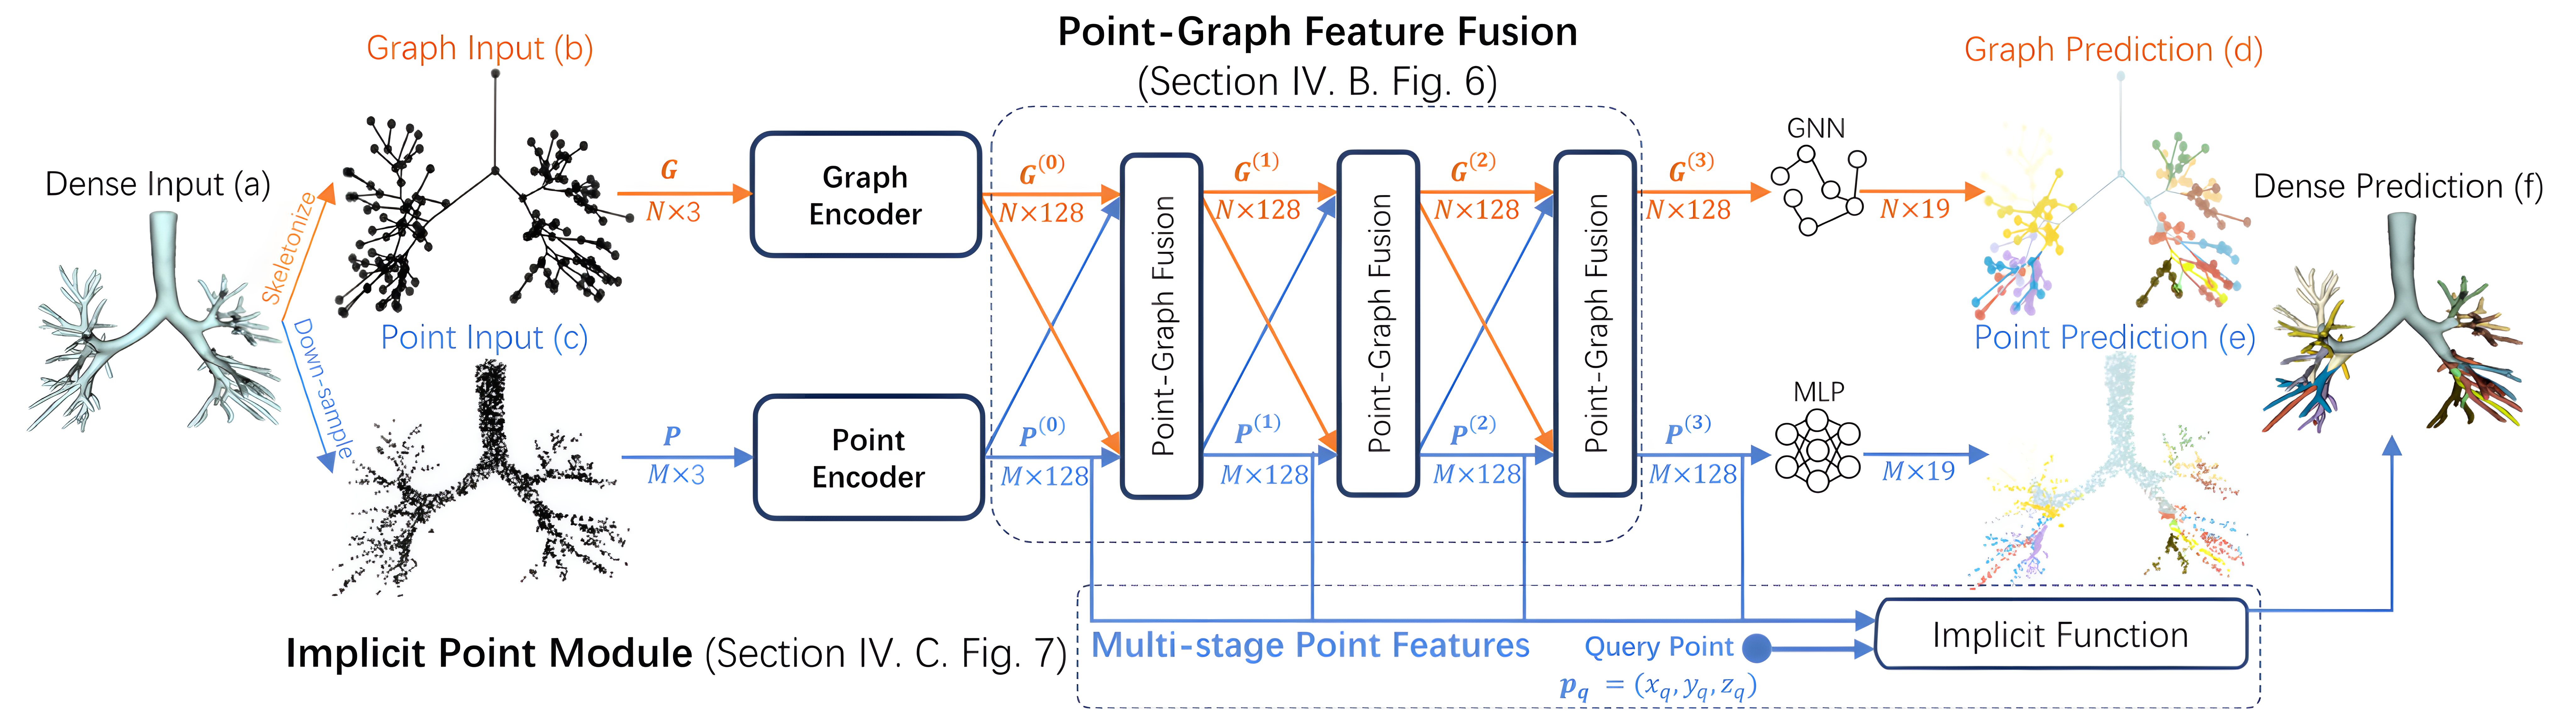
\includegraphics[width=\textwidth]{figures/ipgn_overview.png}  % uncomment with your file
  \fbox{\parbox[c][4cm][c]{0.9\textwidth}{\centering [IPGN overview figure]}}  % remove once image added
  \caption{Overview of the Implicit Point-Graph Network (IPGN), adapted from
           \citet{xie2025}. The binary volume is converted into a skeleton graph and a
           point cloud, Point-Graph Fusion layers exchange features between the two
           branches, and the Implicit Point Module produces the dense labeled volume.}
  \label{fig:ipgn_overview}              % referenced as Figure~\ref{fig:ipgn_overview}
\end{figure}

\begin{figure}[htbp]                     % placeholder for the fusion-layer figure
  \centering                             % center the figure
  % \includegraphics[width=\textwidth]{figures/ipgn_fusion_layer.png}  % uncomment with your file
  \fbox{\parbox[c][4cm][c]{0.9\textwidth}{\centering [Point-Graph Fusion layer figure]}}  % remove once image added
  \caption{A Point-Graph Fusion layer, adapted from \citet{xie2025}. Graph nodes gather point
           features by ball query and grouping; points gather graph features by
           $k$-nearest-neighbor feature propagation.}
  \label{fig:ipgn_fusion}                % referenced as Figure~\ref{fig:ipgn_fusion}
\end{figure}

% ------------------------------------------------------------------------------
\subsection{Training}                    % how the released weights were obtained
\label{sec:labeling_training}            % \secref{sec:labeling_training}

The released model was trained by Xie et al.\ in two stages \cite{xie2025}.

\paragraph{Encoder pre-training.}        % encoders trained separately and frozen
First, the point encoder and the graph encoder were trained independently on the point and
graph versions of the 19-class labeling task, and then frozen. The point encoders were
trained for 120 epochs with a learning rate of 0.002, and the GAT graph encoder for 240
epochs with a learning rate of 0.02 \cite{xie2025}.

\paragraph{Joint training.}              % PGN + implicit module trained together
Second, PGN and the Implicit Point Module were trained together. In each step, PGN is run on
$M = 6{,}000$ sampled points and the $N$ graph nodes, producing multi-stage features and
predictions for all of them. A second, independent set of $M' = 6{,}000$ foreground points
is then sampled and passed through the Implicit Point Module as query points. The
cross-entropy loss is applied to all $M + M'$ point predictions and all $N$ graph
predictions \cite{xie2025}. This stage ran for 100 epochs with a learning rate of 0.01,
halved every 45 epochs. Random rotation, shifting and scaling were used as data augmentation
to avoid overfitting \cite{xie2025}.

% ------------------------------------------------------------------------------
\subsection{Inference}                   % how the labels on our trees are produced
\label{sec:labeling_inference}           % \secref{sec:labeling_inference}

Inference follows the procedure of \citet{xie2025}:
\begin{enumerate}                        % the inference steps
  \item \textbf{Pre-processing.} The binary airway volume is skeletonized to obtain the
        skeleton graph (\secref{sec:labeling_data}), and 6,000 foreground voxels are
        randomly sampled as the point cloud.
  \item \textbf{Point-Graph Network.} A single forward pass of PGN on the graph and point
        cloud gives the multi-stage point features and the labels of the graph nodes.
  \item \textbf{Dense labeling.} All remaining foreground voxels are grouped into batches
        and passed through the Implicit Point Module as query points, which gives a label
        for every voxel of the tree.
\end{enumerate}
Because PGN only runs once, dense labeling is fast: the authors report around 1.3~s per
airway tree with a PointNet++ encoder and 2.3~s with Point Transformer, against 5.7~s and
12.1~s when PGN is run repeatedly over the whole volume \cite{xie2025}.

% ------------------------------------------------------------------------------
\subsection{Reported performance}        % metrics and results from the paper
\label{sec:labeling_performance}         % \secref{sec:labeling_performance}

Xie et al.\ evaluate the model with micro-averaged Dice scores, chosen because of the class
imbalance, at two levels \cite{xie2025}. At the \emph{voxel level}, the Dice score measures
the overlap between the predicted and ground-truth labeled volumes and reflects overall
performance. At the \emph{graph level}, the Dice score is computed on the labels of the
skeleton nodes and edges and reflects performance at the key locations of the tree.

Table~\ref{tab:ipgn_results} summarizes the results reported for the airway tree on the PTL
test set. IPGN outperforms CNN, point-based and graph-based baselines at both levels, and its
dense predictions from the Implicit Point Module are almost identical to those of the full
PGN \cite{xie2025}.

\begin{table}[htbp]                      % airway results reported by Xie et al.
  \centering                             % center the table
  \small                                 % slightly smaller font so the table fits
  \caption{Airway labeling results on the PTL test set as reported by \citet{xie2025}:
           micro-averaged Dice at voxel and graph (node, edge) level, and dense inference
           time per tree.}
  \label{tab:ipgn_results}               % referenced as Table~\ref{tab:ipgn_results}
  \begin{tabular}{lcccc}                 % method + 3 Dice columns + time
    \toprule
    Method & Voxel (\%) & Node (\%) & Edge (\%) & Time (s) \\
    \midrule
    3D U-Net (down-sampled)  & 58.5 & 61.3 & 62.3 & 8.16 \\
    Point Transformer        & 87.8 & 87.2 & 87.4 & 10.97 \\
    GAT                      & 86.3 & 92.7 & 89.1 & 1.15 \\
    IPGN (PointNet++)        & 87.5 & 95.1 & 92.3 & 1.30 \\
    IPGN (Point Transformer) & 88.5 & 95.0 & 92.7 & 2.32 \\
    \bottomrule
  \end{tabular}
\end{table}

% ------------------------------------------------------------------------------
\subsection{Application to our airway trees}  % what was actually done on our data
\label{sec:labeling_ours}                % \secref{sec:labeling_ours}

We applied the released IPGN model with the \TODO{PointNet++ / Point Transformer} encoder to
our \TODO{number} airway trees. Each tree was \TODO{binarized and resampled to \ldots},
skeletonized with VesselVio, and labeled following the inference procedure described in
\secref{sec:labeling_inference}. Examples of the labeled trees are shown in
Figure~\ref{fig:ipgn_ours}. \TODO{Since our data has no ground-truth segmental labels, the
predictions were assessed visually / against \ldots} The resulting labels are used in
\secref{sec:morphometrics} to compute the morphological descriptors of each anatomical class.

\begin{figure}[htbp]                     % placeholder for labeled trees from our data
  \centering                             % center the figure
  % \includegraphics[width=\textwidth]{figures/ipgn_our_labels.png}  % uncomment with your file
  \fbox{\parbox[c][4cm][c]{0.9\textwidth}{\centering [Our airway trees labeled by IPGN]}}
  \caption{Anatomical labels predicted by IPGN on examples of our airway trees. Colours
           denote the 19 classes.}
  \label{fig:ipgn_ours}                  % referenced as Figure~\ref{fig:ipgn_ours}
\end{figure}

\section[Morphological Metrics]{Morphological Analysis of Airway Trees}
\label{sec:morphometrics}                % \secref{sec:morphometrics} -- used by the Labelling section
\label{sec:morph}                        % same place, name used in the draft

Once every airway tree is anatomically labeled (\secref{sec:labeling}), we describe its shape
with the six morphological descriptors of AirwaySignature, introduced with the AirMorph
framework by \citet{zhang2025airmorph}: Stenosis ($S$), Ectasia ($E$), Tortuosity ($T$),
Length ($L$), Divergence ($D$) and Complexity ($C$). The descriptors capture local variations
in airway shape that cannot be seen from the binary segmentation alone and they are defined
per anatomical class, so that each value refers to a specific bronchus (a segmental or a
lobar branch) \cite{zhang2025airmorph}. For each tree, the result is a compact, anatomically
aligned signature, one value of each descriptor for every anatomical class present in the
tree Figure~\ref{fig:morph_ours}..

% ------------------------------------------------------------------------------
\subsection{Overview}                    % the two groups of descriptors
\label{sec:morph_overview}               % \secref{sec:morph_overview}

\citet{zhang2025airmorph} divide the six descriptors into two groups
(Figure~\ref{fig:morph_def}):
\begin{itemize}                          % the two descriptor groups
  \item \textbf{Branch-level descriptors} ($S$, $E$, $T$) are first computed on each
        individual branch of the airway skeleton and then averaged over all branches that
        belong to the same anatomical class. Stenosis measures the strongest narrowing
        of a branch, Ectasia its strongest dilation, and Tortuosity how much its 3D
        trajectory bends.
  \item \textbf{Subtree-level descriptors} ($L$, $D$, $C$) are computed on the whole
        subtree of an anatomical class, i.e.\ on all connected branches that share the same
        anatomical context. Length measures the geodesic length of the subtree,
        Divergence the angular spread of its terminal branches, and Complexity the
        irregularity and density of its branching through a fractal dimension.
\end{itemize}
The anatomical class $K$ over which the descriptors are grouped can be a segmental or a
lobar bronchus \cite{zhang2025airmorph}. In our case the labels come from IPGN, which
provides 18 segmental classes. The lobar classes were obtained by merging the segmental
labels of each lobe / we computed the descriptors at segmental level only.

Table~\ref{tab:morph_summary} summarizes the six descriptors.

\begin{table}[htbp]                      % summary of the six descriptors
  \centering                             % center the table
  \small                                 % slightly smaller font so the table fits
  \caption{The six AirwaySignature descriptors of \citet{zhang2025airmorph}.}
  \label{tab:morph_summary}              % referenced as Table~\ref{tab:morph_summary}
  \begin{tabular}{llll}                  % name, level, range, higher value means
    \toprule
    Descriptor & Computed on & Range & Higher value means \\
    \midrule
    Stenosis ($S$)    & Each branch, then averaged & $[0\%, 100\%]$ & stronger narrowing \\
    Ectasia ($E$)     & Each branch, then averaged & $[100\%, +\infty)$ & stronger dilation \\
    Tortuosity ($T$)  & Each branch, then averaged & $[0, 1]$ & stronger bending \\
    Length ($L$)      & Class subtree & $[0, +\infty)$ mm & longer subtree \\
    Divergence ($D$)  & Class subtree & $[0, 1]$ & wider angular spread \\
    Complexity ($C$)  & Class subtree & $[0, +\infty)$ & more complex branching \\
    \bottomrule
  \end{tabular}
\end{table}

\begin{figure}[htbp]                     % placeholder for the descriptor definition figure
  \centering                             % center the figure
  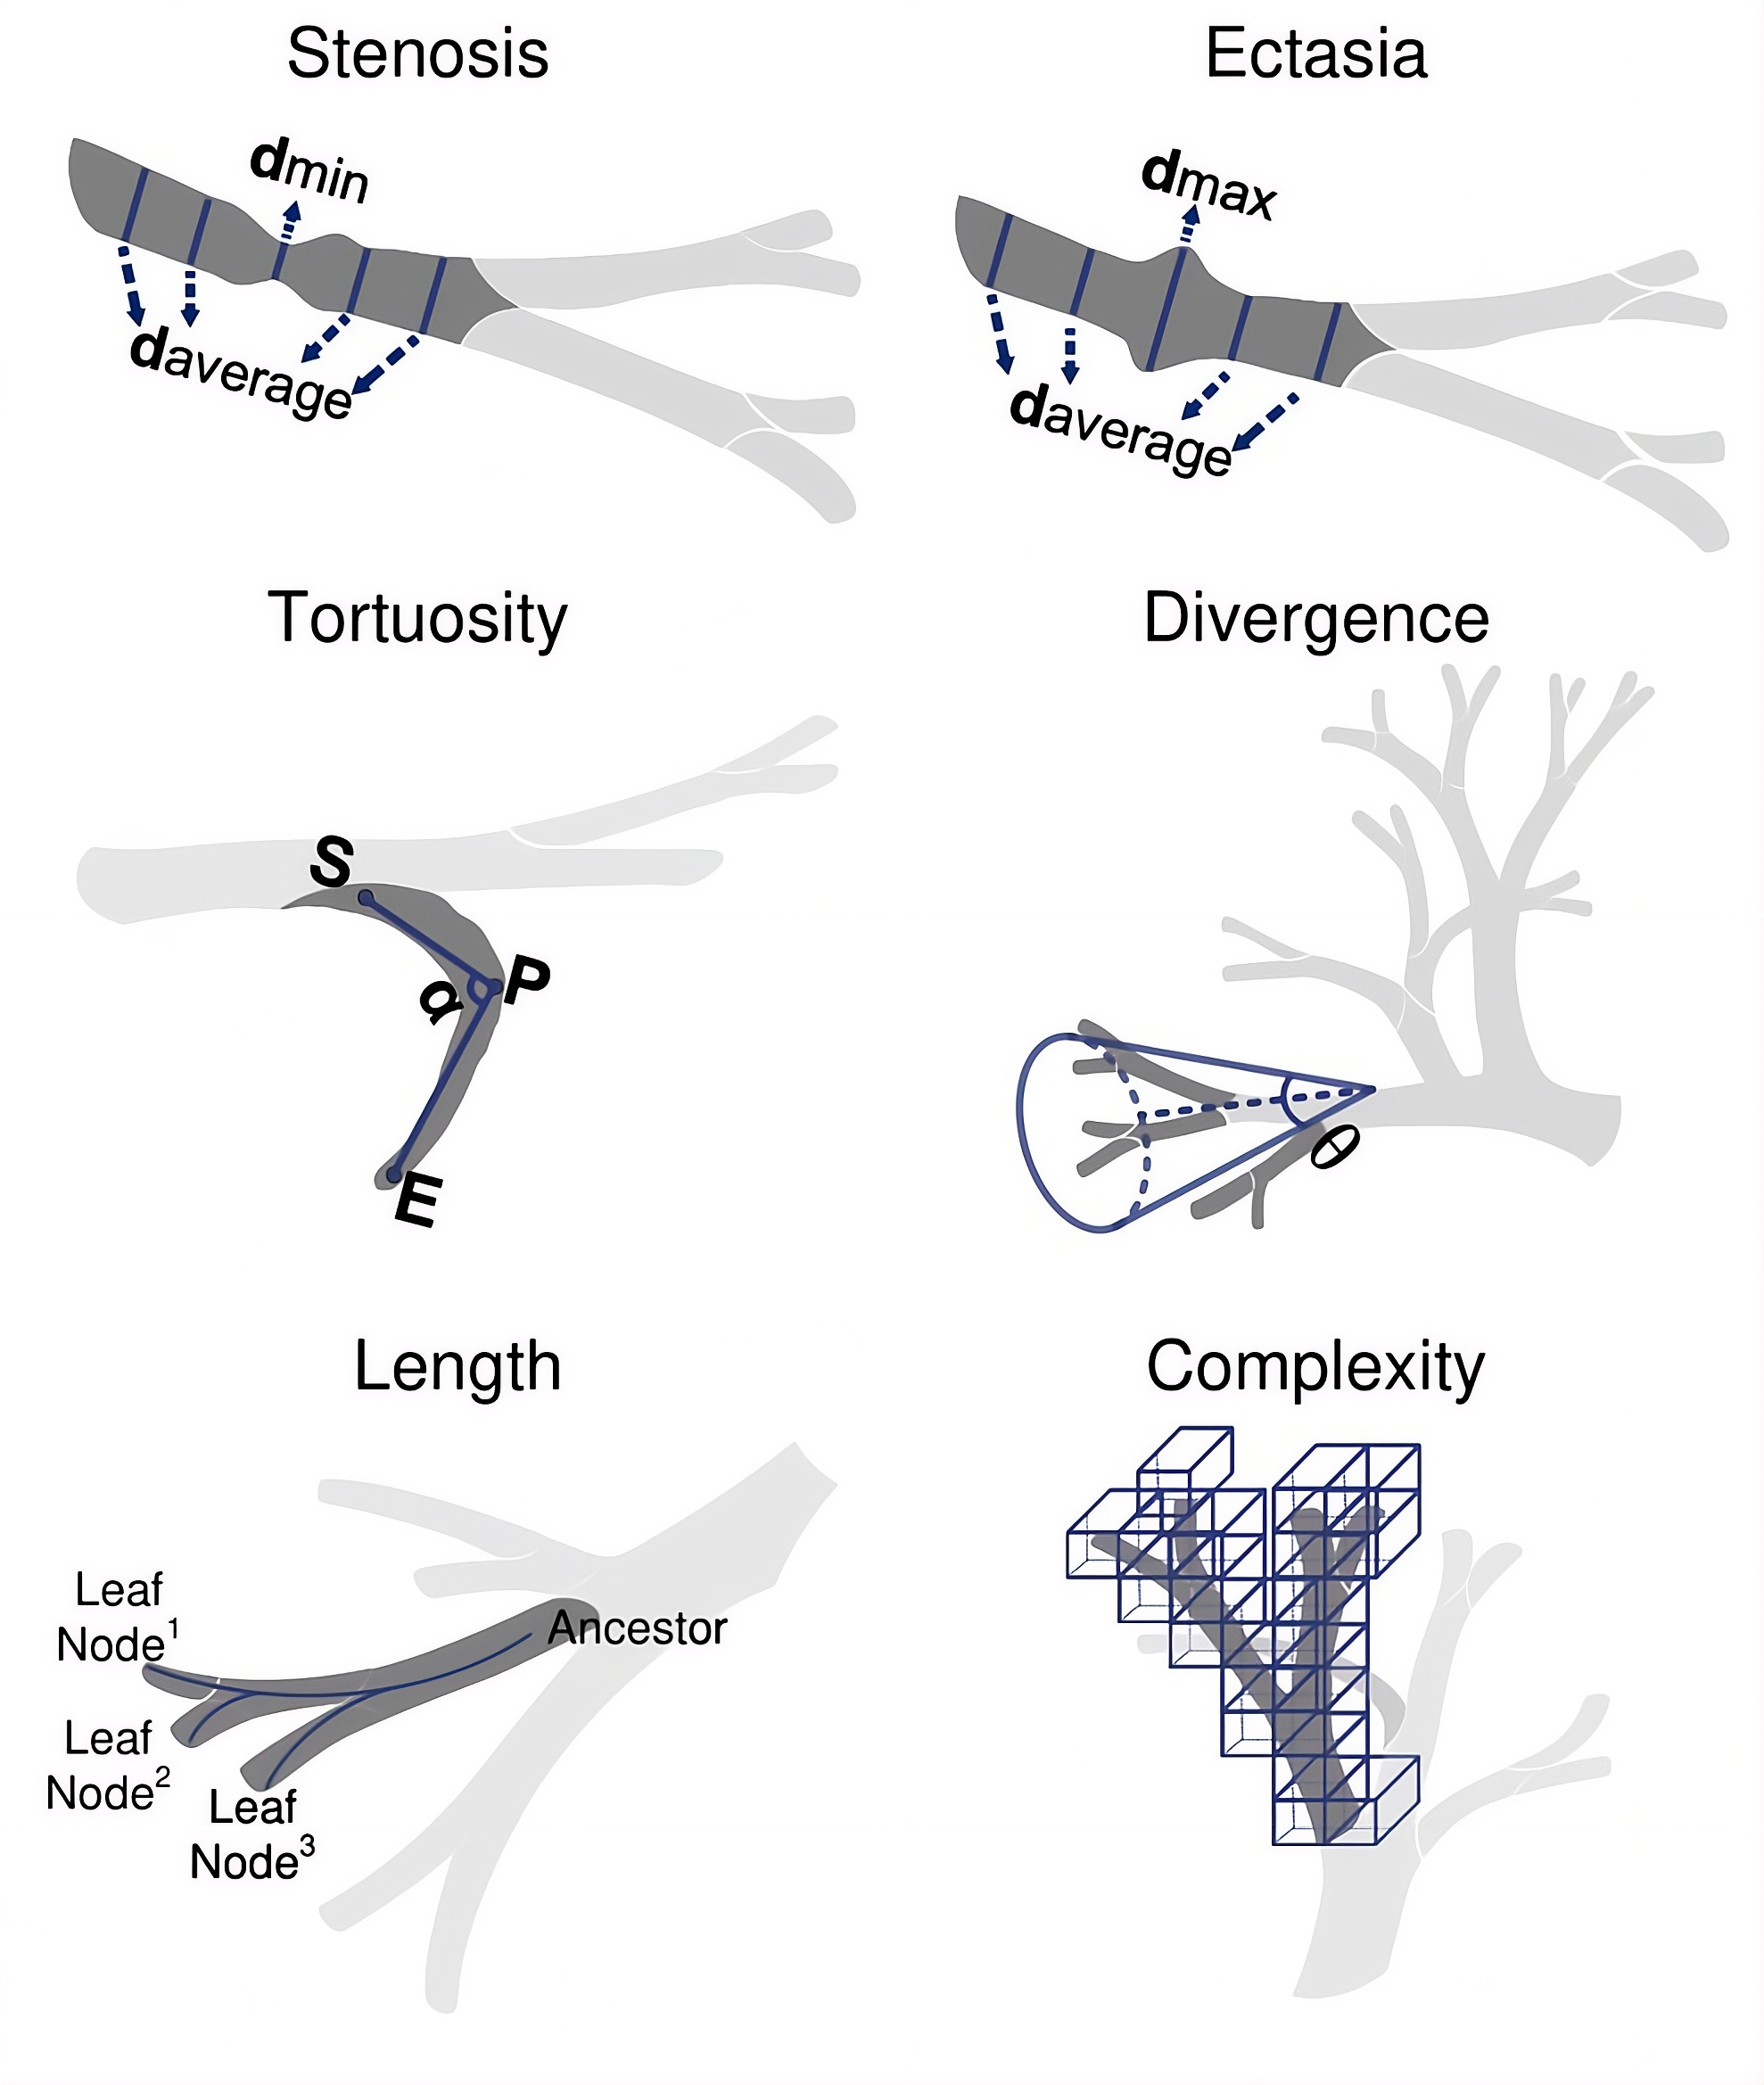
\includegraphics[width=\textwidth]{figures/morphological_metrics.png}  % uncomment with your file
  \caption{The six morphological descriptors of AirwaySignature from
           \citet{zhang2025airmorph}.}
  \label{fig:morph_def}                  % referenced as Figure~\ref{fig:morph_def}
\end{figure}

% ------------------------------------------------------------------------------
\subsection{Common pre-processing}       % radius field and skeleton parsing
\label{sec:morph_preproc}                % \secref{sec:morph_preproc}

Stenosis and Ectasia are both based on the local airway radius along the centerline, which is
obtained as follows \cite{zhang2025airmorph}:
\begin{enumerate}                        % the radius-extraction steps
  \item \textbf{Radius field.} A 3D Euclidean distance transform (EDT) is applied to the
        binary airway mask $V_{\mathrm{airway}}$, taking the voxel spacing $s$ into
        account. At every foreground voxel it gives the distance to the nearest background
        voxel, i.e.\ an approximation of the local airway radius in mm.
  \item \textbf{Centerline radii.} The distance field is masked with the airway skeleton
        $\mathcal{S}$, keeping only the values on centerline voxels. This gives the
        radius field along the skeleton:
        \begin{equation}
          R = \mathrm{EDT}(V_{\mathrm{airway}}; s) \cdot \mathcal{S}.
          \label{eq:morph_radius}        % radius restricted to the skeleton
        \end{equation}
  \item \textbf{Skeleton parsing.} The skeleton is split into individual branches using a
        26-connected neighborhood and removing the junction voxels, so that each branch is
        spatially isolated. Each parsed branch $b$ receives the anatomical label of the
        region it lies in.
\end{enumerate}
For every parsed branch $b$, the minimum, mean and maximum radius along its centerline are
then computed:
\begin{equation}
  r^{(b)}_{\min} = \min_{x \in b} R(x), \qquad
  r^{(b)}_{\mathrm{mean}} = \frac{1}{|b|} \sum_{x \in b} R(x), \qquad
  r^{(b)}_{\max} = \max_{x \in b} R(x).
  \label{eq:morph_rstats}                % per-branch radius statistics
\end{equation}

% ------------------------------------------------------------------------------
\subsection{Branch-level descriptors}    % stenosis, ectasia, tortuosity
\label{sec:morph_branch}                 % \secref{sec:morph_branch}

\paragraph{Stenosis ($S$).}              % narrowing
Stenosis quantifies airway narrowing. \citet{zhang2025airmorph} define it as the reduction of
the radius at the point of strongest constriction, $R_{\mathrm{narrow}}$, relative to a
reference radius $R_{\mathrm{ref}}$, the mean radius of a healthy proximal airway segment:
\begin{equation}
  \mathrm{Stenosis} = \left(1 - \frac{R_{\mathrm{narrow}}}{R_{\mathrm{ref}}}\right)
  \times 100\%.
  \label{eq:morph_stenosis_def}          % conceptual stenosis definition
\end{equation}
In their implementation, both quantities are taken from the radius statistics of each
parsed branch: $R_{\mathrm{narrow}}$ is the branch's minimum radius and $R_{\mathrm{ref}}$
its mean radius, which gives the local stenosis ratio of branch $b$:
\begin{equation}
  S_b = 1 - \frac{r^{(b)}_{\min}}{r^{(b)}_{\mathrm{mean}}}.
  \label{eq:morph_stenosis_branch}       % per-branch stenosis as implemented
\end{equation}
The stenosis of an anatomical class $K$ is the average over all branches carrying that label:
\begin{equation}
  S_K = \frac{1}{|B_K|} \sum_{b \in B_K} S_b,
  \label{eq:morph_stenosis_class}        % class-level stenosis
\end{equation}
where $B_K$ is the set of parsed branches with label $K$. If a class is absent from the tree,
its score is set to $-1$ \cite{zhang2025airmorph}. Stenosis ranges from 0\% to 100\%, and
higher values mean a more severe narrowing.

\paragraph{Ectasia ($E$).}               % dilation
Ectasia complements Stenosis: instead of narrowing, it captures over-expansion of the airway
lumen \cite{zhang2025airmorph}. It is defined as the ratio between the maximum radius and the
reference radius, which in the implementation is again the mean radius of each parsed branch:
\begin{equation}
  \mathrm{Ectasia} = \frac{R_{\max}}{R_{\mathrm{ref}}} \times 100\%,
  \qquad
  E_b = \frac{r^{(b)}_{\max}}{r^{(b)}_{\mathrm{mean}}}.
  \label{eq:morph_ectasia}               % per-branch ectasia
\end{equation}
As for Stenosis, the class value $E_K$ is the average of $E_b$ over all branches with label
$K$, and absent classes receive $-1$. Ectasia ranges from 100\% upwards, and higher values
mean a stronger dilation \cite{zhang2025airmorph}.

\paragraph{Tortuosity ($T$).}            % bending of a branch
Tortuosity describes the local curvature of a branch from its volumetric
geometry \cite{zhang2025airmorph}. For a branch region $\Omega_l$ (the set of its voxels):
\begin{enumerate}                        % the tortuosity steps
  \item the voxel coordinates are converted to physical space using the voxel spacing;
  \item principal component analysis (PCA) is applied to these coordinates, and the two
        endpoints $\mathbf{S}$ and $\mathbf{E}$ of the branch are taken along the first
        principal axis, i.e.\ the main direction of the branch;
  \item the voxel $\mathbf{P}$ that lies furthest from the segment $\overline{SE}$ is
        found:
        \begin{equation}
          \mathbf{P} = \arg\max_{\mathbf{x}_i \in \Omega_l}
              \mathrm{dist}\big(\mathbf{x}_i, \overline{SE}\big);
          \label{eq:morph_tort_p}        % furthest point from the chord
        \end{equation}
  \item the tortuosity is the angle formed at $\mathbf{P}$ by the vectors pointing to the
        two endpoints:
        \begin{equation}
          T = \alpha = \angle\big(\overrightarrow{PS}, \overrightarrow{PE}\big)
            = \arccos \frac{\overrightarrow{PS} \cdot \overrightarrow{PE}}
                           {\|\overrightarrow{PS}\|\,\|\overrightarrow{PE}\|}.
          \label{eq:morph_tort_alpha}    % bending angle at P
        \end{equation}
\end{enumerate}
This angle reflects how much the branch bends or deflects. It lies in $[0, \pi]$ and is then
normalized to $[0, 1]$, with values close to 1 indicating a high degree of
tortuosity \cite{zhang2025airmorph}. As for Stenosis and Ectasia, the class value $T_K$ is the average over
all branches with label $K$.

% ------------------------------------------------------------------------------
\subsection{Subtree-level descriptors}   % length, divergence, complexity
\label{sec:morph_subtree}                % \secref{sec:morph_subtree}

The remaining three descriptors work on the centerline tree, in which each node carries an
anatomical label, a generation number (its depth in the tree) and a length. For each class
$K$, they first identify all terminal (leaf) nodes labeled $K$, denoted $T_K$, and their
lowest common ancestor (LCA), found by a generation-aware traversal of the
tree \cite{zhang2025airmorph}. The LCA is the node where the subtree of class $K$ begins.

\paragraph{Length ($L$).}                % geodesic length of the subtree
Length measures the geometric elongation of a segment or lobe as a geodesic length,
accumulated branch by branch along the skeleton \cite{zhang2025airmorph}. If the LCA itself
belongs to class $K$, the length is the average, over all leaves of class $K$, of the path
length from the LCA to that leaf:
\begin{equation}
  L_K = \frac{1}{|T_K|} \sum_{v \in T_K} \;\sum_{n \in \mathrm{Path}(\mathrm{LCA}, v)}
  \ell(n),
  \label{eq:morph_length}                % mean geodesic path length
\end{equation}
where $\mathrm{Path}(\mathrm{LCA}, v)$ is the set of nodes on the path from the LCA to leaf
$v$ and $\ell(n)$ is the length of node $n$. If the LCA does not belong to class $K$ (for
example, when it is the trachea), each path is re-rooted at the nearest downstream node
labeled $K$, so that only the part of the tree belonging to class $K$ is
measured \cite{zhang2025airmorph}. Length is expressed in mm and ranges from 0 upwards.

\paragraph{Divergence ($D$).}            % angular spread of the leaves
Divergence measures the spatial dispersion of the branches of a class, i.e.\ how widely
they spread from their common origin, using the smallest cone that encloses
them \cite{zhang2025airmorph}. The LCA of the class-$K$ leaves is taken as the apex of the
cone, and $\mathbf{v}_i$ is the normalized direction vector from the apex to leaf $i$. The
axis of the cone is the unit vector $\mathbf{u}^*$ that maximizes the smallest cosine
similarity with all leaf directions:
\begin{equation}
  \mathbf{u}^* = \arg\max_{\|\mathbf{u}\|=1} \; \min_i \,\langle \mathbf{u},
  \mathbf{v}_i \rangle.
  \label{eq:morph_div_axis}              % optimal cone axis
\end{equation}
The divergence angle is twice the largest angular deviation of a leaf direction from this
axis, i.e.\ the full opening angle of the enclosing cone:
\begin{equation}
  \theta = 2 \cdot \arccos\Big(\min_i \,\langle \mathbf{u}^*, \mathbf{v}_i \rangle\Big).
  \label{eq:morph_div_theta}             % cone opening angle
\end{equation}
The angle lies in $[0, \pi]$ and is normalized to $[0, 1]$. A smaller angle means that the
branches of the class are less separated and less angularly dispersed, which can be affected
by pulmonary disease \cite{zhang2025airmorph}.

\paragraph{Complexity ($C$).}            % box-counting fractal dimension
Complexity measures the geometric complexity of the branches of a class with a box-counting
fractal dimension, which captures the spatial irregularity and branching density of the
skeleton \cite{zhang2025airmorph}. For each class $K$:
\begin{enumerate}                        % the box-counting steps
  \item the skeleton voxels labeled $K$ are extracted as a binary mask,
        $\mathcal{S}_K = (\mathcal{S} > 0) \wedge (Y = K)$;
  \item this mask is cropped to its bounding box and zero-padded to a fixed 3D size;
  \item the volume is covered with cubic boxes of sizes $s \in \{2^1, 2^2, \dots, 2^k\}$,
        and for each size the number $N(s)$ of boxes containing at least one skeleton voxel
        is counted.
\end{enumerate}
The complexity is the box-counting dimension
\begin{equation}
  C = \lim_{s \to 0} \frac{\log N(s)}{\log(1/s)},
  \label{eq:morph_complexity}            % box-counting dimension
\end{equation}
estimated in practice as the slope of a linear regression of $\log N(s)$ against
$\log(1/s)$ \cite{zhang2025airmorph}. A straight line has a dimension close to 1, while a
densely branching structure that fills more of the space has a higher value. Complexity
ranges from 0 upwards, and larger values denote a more complex branching pattern.

\begin{figure}[htbp]                     % placeholder for our signatures
  \centering                             % center the figure
  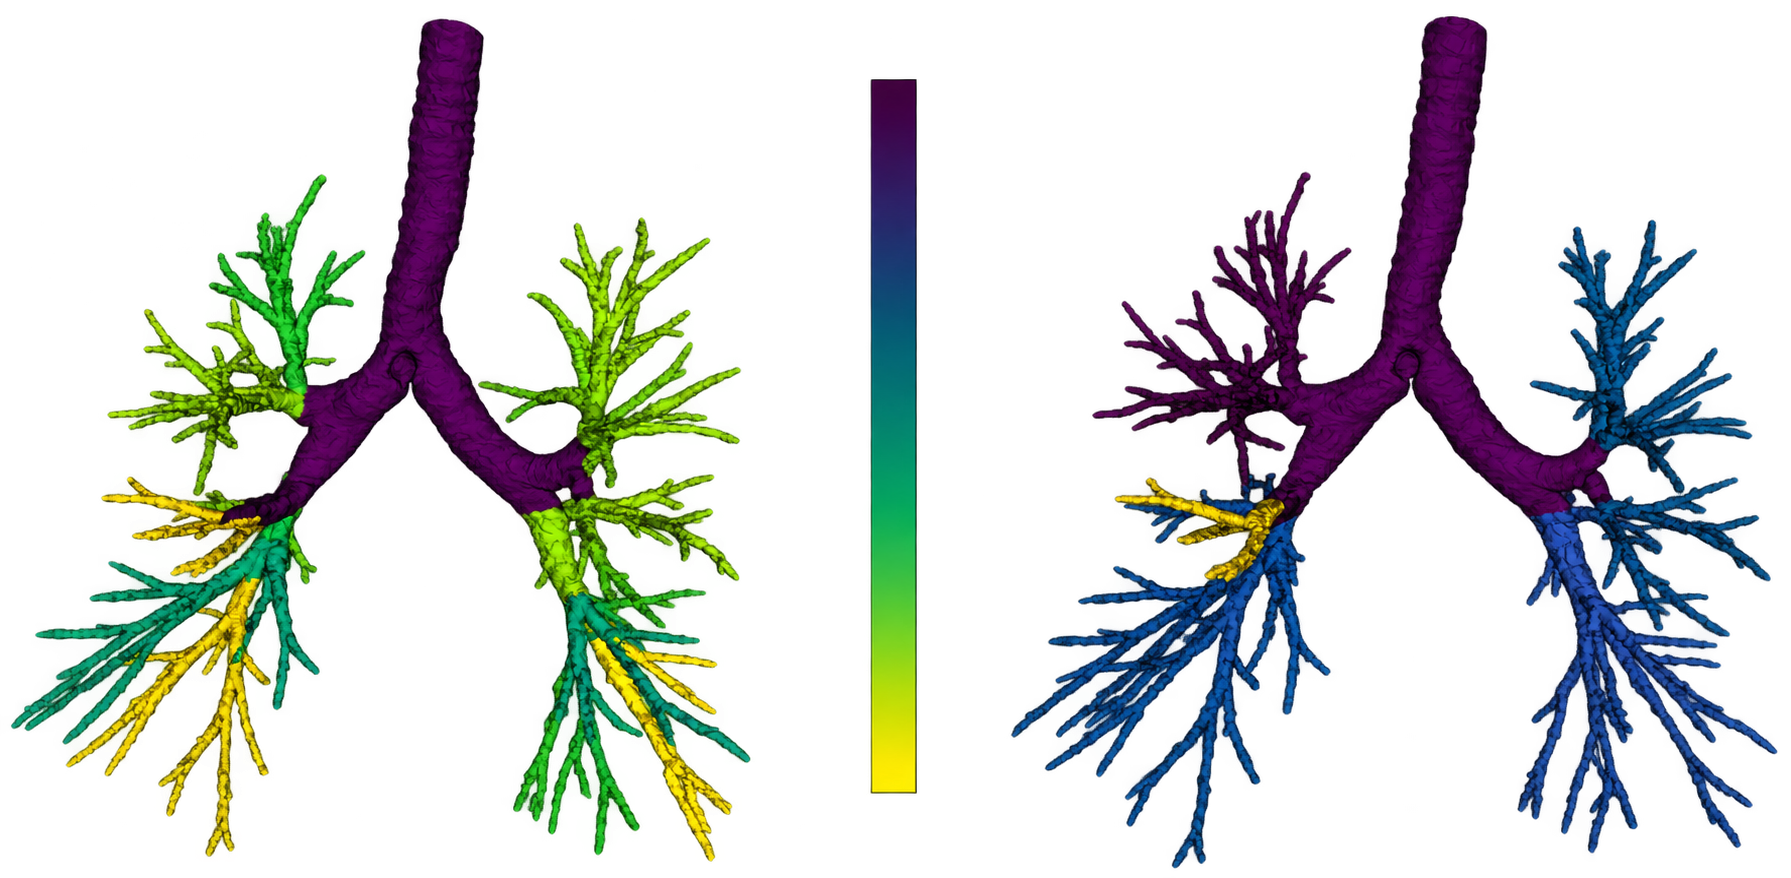
\includegraphics[width=\textwidth]{figures/morph_signatures_ours.png}  % uncomment with your file
  \caption{Examples of airway trees visualized according to the Ectasia descriptor of
            AirwaySignature \cite{zhang2025airmorph}. The left panel shows Ectasia values computed
            at the segmental level, with each color corresponding to an individual segmental
            bronchial class. The right panel shows the same descriptor computed at the lobar level,
            after grouping the corresponding segmental branches within each lobe. The common color
            scale indicates the magnitude of ectasia, with warmer colors corresponding to greater
            airway dilation relative to the mean branch radius.}
  \label{fig:morph_ours}                 % referenced as Figure~\ref{fig:morph_ours}
\end{figure}

% Clustering -- parent section; each part is a subsection in its own file.

\section{Clustering}                     % phenotype discovery in the latent space
\label{sec:clustering}                   % \secref{sec:clustering} -- used by Encoding and Morphological Metrics

The implicit model of represents every airway tree by a latent code. If
groups of trees with a similar shape exist, they should appear as groups of nearby codes. Following
the phenotype-discovery approach of \citet{norouzi2024volpam}, who cluster the latent codes of a
3D autoencoder to find imaging phenotypes without any labels, we cluster the latent codes of the
airway trees with two families of methods: agglomerative hierarchical clustering and K-means,
the latter also in a kernel version. The groups found are then visualized with three
projections of the latent space and characterized with the morphological descriptors of
\secref{sec:morphometrics} (Figure~\ref{fig:clustering_pipeline}).

\begin{figure}[htbp]                     % the clustering pipeline at a glance
  \centering                             % center the diagram
  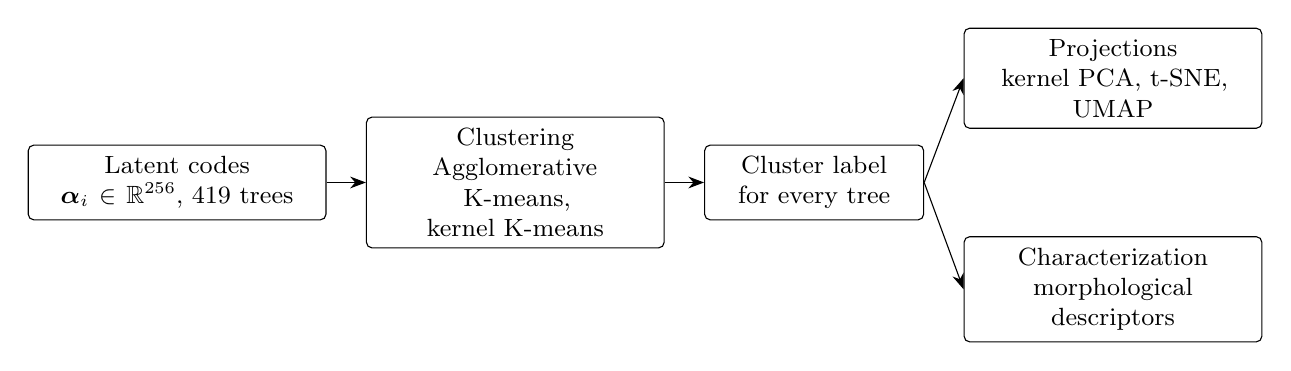
\begin{tikzpicture}[
      node distance=5mm and 5mm,                         % vertical and horizontal gaps
      box/.style={draw, rounded corners=2pt, align=center, text width=3.5cm,
                  inner sep=4pt, font={\small\hyphenpenalty=10000}},  % one box per step, no hyphens
      arr/.style={-{Stealth[length=2mm]}}]               % arrow style
    \node[box] (codes) {Latent codes\\$\boldsymbol{\alpha}_i \in \mathbb{R}^{256}$, 419 trees};
    \node[box, right=of codes] (clus) {Clustering\\Agglomerative\\K-means, kernel K-means};
    \node[box, right=of clus, text width=2.5cm] (lab) {Cluster label\\for every tree};
    \node[box, above right=2mm and 5mm of lab] (proj) {Projections\\kernel PCA, t-SNE,\\UMAP};
    \node[box, below right=2mm and 5mm of lab] (morph) {Characterization\\morphological descriptors};
    \draw[arr] (codes) -- (clus);                         % codes are clustered
    \draw[arr] (clus) -- (lab);                           % clustering gives labels
    \draw[arr] (lab.east) -- (proj.west);                 % labels coloured in the projections
    \draw[arr] (lab.east) -- (morph.west);                % labels compared with the descriptors
  \end{tikzpicture}
  \caption{Clustering pipeline. The latent codes are clustered in their full space; the
           projections are only used to look at the result, and the morphological descriptors
           to describe what distinguishes the clusters.}
  \label{fig:clustering_pipeline}        % referenced as Figure~\ref{fig:clustering_pipeline}
\end{figure}

% % % Input of the clustering: the DGCI latent codes. Subsection of "Clustering".

% \subsection{Input: the latent codes}     % what is clustered
% \label{sec:clust_input}                  % \secref{sec:clust_input}

% After training, every airway tree $i$ is represented by its instance latent code
% $\boldsymbol{\alpha}_i \in \mathbb{R}^{128}$ (\secref{sec:dgci_training}). Stacking the codes of
% the $N = 419$ trees gives the data matrix $X \in \mathbb{R}^{419 \times 128}$, whose rows
% $\mathbf{x}_i = \boldsymbol{\alpha}_i$ are the points to cluster. All distances below are
% Euclidean distances between these codes.

% \paragraph{Active dimensions}            % not every latent dimension carries information
% Not every latent dimension is used by the model: the regularization of the latent codes
% (Eq.~\eqref{eq:dgci_reg}) pulls them towards the shared code, so dimensions that do not help the
% reconstruction stay almost constant across trees. To measure how much each dimension varies, we
% use its median absolute deviation (MAD), a spread measure that is not driven by a few outlying
% shapes,
% \begin{equation}
%   \mathrm{MAD}_j = \operatorname{median}_i \big|\, x_{ij} - \operatorname{median}_k x_{kj} \,\big|,
%   \qquad j = 1, \dots, 128.
%   \label{eq:mad}                         % robust spread of latent dimension j
% \end{equation}
% Sorted on a logarithmic scale, the MAD values show a clear gap between active and nearly
% constant dimensions; with a threshold of $3 \times 10^{-4}$ placed in this gap, about 45
% dimensions are active. \TODO{State which input was used for each method: all 128 dimensions,
% or only the active ones. In the notebooks, agglomerative clustering uses all 128; in the
% K-means notebook the final assignment \texttt{codes\_active = enc\_output} also selects all 128.}
   % Subsection "Input: the latent codes"
% Agglomerative hierarchical clustering (Ward). Subsection of "Clustering".

\subsection{Agglomerative hierarchical clustering}  % bottom-up merging, Ward linkage
\label{sec:clust_agglo}                  % \secref{sec:clust_agglo}

% \paragraph{Principle}                    % bottom-up construction of a hierarchy
Agglomerative clustering builds a hierarchy of nested groups from the bottom up
\cite{norouzi2024volpam}. At the start, every tree is a cluster of its own. At each step, the two
closest clusters are merged, and the procedure repeats until a single cluster contains all the
trees. The sequence of merges forms a binary tree, the \emph{dendrogram}, in which the height of
each junction shows how far apart the two merged clusters were. Cutting the dendrogram with a
horizontal line at some height gives a partition into $K$ clusters, so one run of the algorithm
yields the clustering for every $K$ and shows how small groups nest inside larger ones. This is
what makes hierarchical methods attractive for discovering intrinsic groupings whose number is
not known in advance \cite{norouzi2024volpam}.

\paragraph{Linkage}                      % how "closest" is defined: Ward
What ``closest'' means is set by the linkage. \citet{norouzi2024volpam} merge the two
clusters whose centroids are closest. We use Ward's linkage \cite{ward1963}, which merges the
pair of clusters whose union increases the total within-cluster sum of squares the least. For
two clusters $A$ and $B$ with centroids $\boldsymbol{\mu}_A$ and $\boldsymbol{\mu}_B$, this
increase is
\begin{equation}
  \Delta(A, B) = \frac{|A|\,|B|}{|A| + |B|}\,
                 \big\|\boldsymbol{\mu}_A - \boldsymbol{\mu}_B\big\|_2^2 .
  \label{eq:ward}                        % cost of merging A and B
\end{equation}
Like the centroid linkage, Ward's criterion compares cluster centres, but the factor in front of
the distance penalizes merging two large clusters, so it favours compact clusters of similar
size. Since it greedily minimizes the same within-cluster sum of squares as K-means
(Eq.~\eqref{eq:kmeans}), the two methods can be compared directly.

\paragraph{Choosing the number of clusters}  % elbow on the average intra-cluster distance
To choose where to cut the dendrogram, we follow the elbow criterion of
\citet{norouzi2024volpam}. For every number of clusters $k = 1, \dots, 19$, we cut the hierarchy
into $k$ clusters and compute the average intra-cluster distance, the mean distance between two
trees of the same cluster, averaged over the clusters:
\begin{equation}
  D_{\mathrm{avg}}(k) = \frac{1}{k} \sum_{l=1}^{k}
     \frac{1}{N_l^2} \sum_{u=1}^{N_l} \sum_{v=1}^{N_l}
     \big\|\mathbf{x}_{ul} - \mathbf{x}_{vl}\big\|_2 ,
  \label{eq:davg}                        % mean pairwise distance inside each cluster
\end{equation}
where $N_l$ is the number of trees in cluster $l$ and $\mathbf{x}_{ul}$ is the code of its
$u$-th tree. Splitting a cluster always makes its parts more compact, so $D_{\mathrm{avg}}$ tends
to decrease with $k$. The useful information is where it drops the most: the number of
clusters is chosen as the one with the largest relative reduction \cite{norouzi2024volpam},
\begin{equation}
  k^{*} = \arg\max_{k}\;
          \frac{D_{\mathrm{avg}}(k-1) - D_{\mathrm{avg}}(k)}{D_{\mathrm{avg}}(k-1)} .
  \label{eq:kstar}                       % largest relative drop of D_avg
\end{equation}
A large relative drop means that going from $k-1$ to $k$ clusters separates groups that are
genuinely different; after that point, further splits mostly cut coherent groups into pieces.
The elbow criterion identified $k^{\*}=4$ as the optimal number of clusters for both the registered and unregistered airway trees. Thus, in both representations, the hierarchy was cut at four clusters for the subsequent analysis.  % Subsection "Agglomerative hierarchical clustering"
% K-means. Subsection of "Clustering".

\subsection{K-means}
\label{sec:clust_kmeans}

Unlike agglomerative clustering, K-means directly partitions the trees into a fixed number $K$ of
clusters. Each cluster $c$ is represented by its centroid $\boldsymbol{\mu}_c$, and the
partition is chosen to minimize the \emph{inertia}, the total squared distance of the trees to
the centroid of their cluster:
\begin{equation}
  J = \sum_{i=1}^{N} \big\|\mathbf{x}_i - \boldsymbol{\mu}_{c(i)}\big\|_2^2 ,
  \label{eq:kmeans}
\end{equation}
where $c(i)$ is the cluster of tree $i$. Lloyd's algorithm \cite{lloyd1982} alternates two
steps: every tree is assigned to its nearest centroid, then every centroid is moved to the mean
of the trees assigned to it. Neither step can increase $J$, so the algorithm converges, but only
to a local minimum that depends on the initial centroids. We therefore initialize the centroids
with k-means++ \cite{arthur2007kmeanspp}, which spreads them out by picking distant trees with
higher probability, and keep the best of 20 runs with different initializations (scikit-learn
implementation \cite{pedregosa2011sklearn}). Because each tree joins its nearest centroid, the
borders between clusters are flat hyperplanes: K-means works best for compact, roughly
spherical clusters.

\paragraph{Choosing the number of clusters}
K-means requires the number of clusters $K$ to be specified in advance. We therefore evaluated
$K=2,\dots,10$ for each airway-tree representation. For each candidate $K$, K-means was fitted
to the 256-dimensional latent codes using k-means++ initialization with 20 restarts, retaining
the solution with the lowest inertia. Two criteria were then evaluated: the inertia, which
measures the within-cluster sum of squared distances, and the silhouette coefficient
\cite{rousseeuw1987silhouettes}, which measures how well each tree is separated from the other
clusters. The mean silhouette was used to assess the separation of the resulting partition.
\begin{equation}
  s(i) = \frac{b(i) - a(i)}{\max\{a(i),\, b(i)\}} \in [-1, 1].
  \label{eq:silhouette}
\end{equation}
The analysis identified $K=3$ as the preferred number of clusters for both the registered and
unregistered airway-tree representations. The final K-means analysis was therefore performed
with three clusters for both representations.         % Subsection "K-means and kernel K-means"
% Projections used to look at the latent space. Subsection of "Clustering".

\subsection{Visualizing the latent space}  % kernel PCA, t-SNE, UMAP
\label{sec:clust_projections}            % \secref{sec:clust_projections}

The latent codes are represented in a 256-dimensional space and therefore cannot be directly
visualized. We project them to two and three dimensions using three complementary dimensionality-
reduction methods and colour the resulting embeddings according to cluster membership or
morphological descriptors.
% The projections are used only for viewing: all clusters are computed in the full latent space and no projection preserves all
% distances, so a separation that appears in a projection, or the lack of one, has to be read with
% care. 
The three methods distort the data in different ways, which is why we compare them.

\paragraph{Kernel PCA}                   % linear PCA in the RBF feature space
Principal component analysis (PCA) finds the orthogonal directions of largest variance; kernel PCA
\cite{scholkopf1998kpca} does the same in the feature space of a kernel. With the RBF kernel of
Eq.~\eqref{eq:rbf}
\begin{equation}
  k(\mathbf{x}_i,\mathbf{x}_j) = \exp\!\left(-\gamma \|\mathbf{x}_i-\mathbf{x}_j\|^2\right)
  \label{eq:rbf}
\end{equation}
and the same median-rule $\gamma$ as kernel K-means, it shows the space in
which kernel K-means operates. The kernel matrix $K$ is first centred,
$\tilde{K} = H K H$ with $H = I - \frac{1}{N}\mathbf{1}\mathbf{1}^{\top}$, and decomposed as
$\tilde{K}\mathbf{v}_m = \lambda_m \mathbf{v}_m$. The coordinate of tree $i$ on the $m$-th
component is $\sqrt{\lambda_m}\, v_{m,i}$, and the share of kernel variance kept by a view with
$d$ components is $\sum_{m \le d} \lambda_m / \sum_m \lambda_m$. 
% Kernel PCA is deterministic and
% keeps the global layout of the data, but it only shows the few directions of largest variance.
% % \TODO{Report the kernel variance shown in 2D and in 3D (printed by the notebook).}

\paragraph{t-SNE}                        % neighbourhood probabilities, KL divergence
t-distributed stochastic neighbour embedding (t-SNE) \cite{vandermaaten2008tsne} preserves
neighbourhoods rather than distances. For every tree $i$, it turns distances into probabilities
of picking tree $j$ as a neighbour,
\begin{equation}
  p_{j|i} = \frac{\exp\!\big(-\|\mathbf{x}_i - \mathbf{x}_j\|^2 / 2\sigma_i^2\big)}
                 {\sum_{k \neq i} \exp\!\big(-\|\mathbf{x}_i - \mathbf{x}_k\|^2 / 2\sigma_i^2\big)} ,
  \label{eq:tsne_p}                      % neighbour probabilities in the latent space
\end{equation}
where the width $\sigma_i$ is chosen so that the distribution has a given \emph{perplexity},
roughly the effective number of neighbours. In the projection, similarities $q_{ij}$ follow a
heavy-tailed Student-$t$ distribution, $q_{ij} \propto (1 + \|\mathbf{y}_i - \mathbf{y}_j\|^2)^{-1}$,
and the points $\mathbf{y}_i$ are moved by gradient descent to minimize the Kullback--Leibler
divergence between the symmetrized $p_{ij}$ and $q_{ij}$. The heavy tail lets dissimilar trees
drift apart, which gives well-separated groups, but the sizes of the groups and the distances
between them are not meaningful. We ran t-SNE with PCA initialization and 1000 iterations, for
perplexities from 5 to 50 in steps of 5.

\paragraph{UMAP}
Uniform Manifold Approximation and Projection (UMAP) \cite{mcinnes2018umap} is a nonlinear
dimensionality reduction method that seeks to preserve the neighbourhood structure of the
high-dimensional data in a lower-dimensional representation. Given the latent codes
$\mathbf{x}_1,\ldots,\mathbf{x}_N$, UMAP first identifies the nearest neighbours of each
observation using the Euclidean distance. These neighbourhood relationships are represented by
a weighted graph.

For each tree $i$, UMAP determines a local connectivity distance $\rho_i$, corresponding to the
distance to the closest neighbour, and a local scale parameter $\sigma_i$. The membership strength
of the connection between tree $i$ and one of its neighbours $j$ is defined as
\begin{equation}
    w_{ij} =
    \begin{cases}
        1, & d(\mathbf{x}_i,\mathbf{x}_j) \leq \rho_i,\\[4pt]
        \exp\!\left(
        -\dfrac{d(\mathbf{x}_i,\mathbf{x}_j)-\rho_i}{\sigma_i}
        \right),
        & d(\mathbf{x}_i,\mathbf{x}_j) > \rho_i,
    \end{cases}
    \label{eq:umap_weight}
\end{equation}
where $d(\mathbf{x}_i,\mathbf{x}_j)$ denotes the Euclidean distance between two latent codes.
Thus, nearby observations receive a high connection strength, while more distant neighbours have
smaller weights. The local scales are chosen so that the graph adapts to the density of the data
around each observation.

UMAP then seeks a low-dimensional representation
$\mathbf{y}_1,\ldots,\mathbf{y}_N$ whose neighbourhood structure reproduces that of the original
graph. In the low-dimensional space, the strength of an association between two observations is
modelled by
\begin{equation}
    \tilde{w}_{ij}
    =
    \frac{1}
    {1+a\|\mathbf{y}_i-\mathbf{y}_j\|_2^{2b}},
    \label{eq:umap_lowdim}
\end{equation}
where $a$ and $b$ determine the shape of the low-dimensional decay function. The embedding is
obtained by minimizing the cross-entropy between the high- and low-dimensional fuzzy graphs:
\begin{equation}
    \mathcal{L}_{\mathrm{UMAP}}
    =
    -\sum_{i,j}
    \left[
        w_{ij}\log(\tilde{w}_{ij})
        +
        (1-w_{ij})\log(1-\tilde{w}_{ij})
    \right].
    \label{eq:umap_loss}
\end{equation}
Minimizing this objective attracts observations that are strongly connected in the original
latent space and repels observations that have weak or no connections. The resulting embedding
therefore preserves neighbourhood relationships rather than the exact pairwise distances of the
original space.

The scale of the neighbourhood structure is controlled by the number of neighbours considered for
each observation. Small values emphasize local structure, whereas larger values allow broader
relationships to influence the embedding. A minimum-distance parameter further controls how
closely neighbouring observations can be placed in the low-dimensional space.

In our experiments, UMAP was applied directly to the 256-dimensional latent representations using
Euclidean distance and the default minimum-distance value. The neighbourhood size was varied
from 5 to 55 in increments of 5, and both two- and three-dimensional embeddings were generated.

% \paragraph{Parameter sweeps}             % trust what is stable across settings
% Because t-SNE and UMAP depend on their parameters and on the random initialization (fixed with a
% seed), we computed them over the whole range of perplexities and neighbour counts, in 2D and 3D.
% A grouping that appears for every setting reflects the data; one that appears for a single
% setting is more likely an artefact of the projection.
    % Subsection "Visualizing the latent space"
% Results of the clustering -- placeholders for figures, tables and interpretation.
% Replace each \figplaceholder by \includegraphics and each \hint by your own text.

\subsection{Results}                     % what the clustering found
\label{sec:clust_results}                % \secref{sec:clust_results}

\subsubsection{Agglomerative clustering}  % dendrogram, elbow, projections
\label{sec:clust_results_agglo}

\begin{figure}[htbp]                     % dendrogram + elbow curve
  \centering
  \figplaceholder[5cm]{Dendrogram of the Ward clustering (last 30 merges), with the cut line}
  \par\medskip
  \figplaceholder[4cm]{Average intra-cluster distance $D_{\mathrm{avg}}(k)$ and its relative reduction}
  \caption{Agglomerative clustering of the latent codes. Top: dendrogram, cut at $k^{*}$
           clusters (dashed line). Bottom: average intra-cluster distance as a function of the
           number of clusters (Eq.~\eqref{eq:davg}) and its relative reduction
           (Eq.~\eqref{eq:kstar}).}
  \label{fig:clust_agglo}
\end{figure}

\hint{Interpret: how many clusters are suggested, how clear is the largest drop compared with the
next candidates, and what are the cluster sizes? Does the dendrogram show well-separated
branches, or merges at similar heights?}

\begin{figure}[htbp]                     % the three projections, coloured by Ward cluster
  \centering
  \figplaceholder[4.5cm]{Kernel PCA \quad|\quad t-SNE \quad|\quad UMAP, coloured by Ward cluster}
  \caption{Latent codes projected with kernel PCA, t-SNE (perplexity \TODO{value}) and UMAP
           (\texttt{n\_neighbors} \TODO{value}), coloured by agglomerative cluster.}
  \label{fig:clust_agglo_proj}
\end{figure}

\hint{Interpret: are the clusters separated in all three projections, only in some, or in none?
Is the picture stable over the parameter sweep?}

\subsubsection{K-means and kernel K-means}  % choice of K, agreement between methods
\label{sec:clust_results_kmeans}

\begin{figure}[htbp]                     % elbow + silhouette for both methods
  \centering
  \figplaceholder[4cm]{K-means and kernel K-means: inertia (elbow) and mean silhouette for $K = 2, \dots, 10$}
  \caption{Choice of the number of clusters for K-means and kernel K-means: inertia
           (Eq.~\eqref{eq:kmeans}) and mean silhouette (Eq.~\eqref{eq:silhouette}).}
  \label{fig:clust_kmeans_k}
\end{figure}

\begin{table}[htbp]                      % agreement between the partitions
  \centering
  \small
  \caption{Agreement between partitions, measured with the adjusted Rand index (1 = same
           partition, 0 = chance level).}
  \label{tab:clust_ari}
  \begin{tabular}{llc}
    \toprule
    Comparison                                   & Latent codes          & ARI \\
    \midrule
    Agglomerative ($K=4$) vs K-means ($K=3$)     & unregistered          & \TODO{?} \\
    Agglomerative ($K=4$) vs K-means ($K=3$)     & registered            & \TODO{?} \\
    K-means: unregistered vs registered          & --                    & \TODO{?} \\
    Agglomerative: unregistered vs registered    & --                    & \TODO{?} \\
    \bottomrule
  \end{tabular}
\end{table}

\hint{Interpret: which $K$ do the elbow and the silhouette suggest, and do they agree? How much do
the two methods, and the two sets of codes, agree (Table~\ref{tab:clust_ari})? Report the robustness checks of
\secref{sec:clust_kmeans}: seed stability (mean ARI), sensitivity to $\gamma$, and the silhouette
of the real data compared with the no-cluster Gaussian baseline.}

\subsubsection{Morphological characterization of the clusters}  % what distinguishes the groups
\label{sec:clust_results_morph}

For every tree, the six descriptors of \secref{sec:morphometrics} are averaged over its branches
and complemented with two whole-tree counts, the number of branches and the deepest generation.
Comparing these eight values between clusters shows what distinguishes the groups, and colouring
the projections by each value shows whether the latent space is organized along these
anatomical properties.

\begin{figure}[htbp]                     % projections coloured by metric
  \centering
  \figplaceholder[5cm]{Projections coloured by each of the 8 metrics}
  \caption{UMAP projection of the latent codes coloured by the mean value of each
           morphological descriptor and by the two tree counts.}
  \label{fig:clust_metric_proj}
\end{figure}

\begin{figure}[htbp]                     % box plots per cluster
  \centering
  \figplaceholder[5cm]{Box plots of the 8 metrics per cluster}
  \caption{Distribution of the eight metrics in each cluster.}
  \label{fig:clust_boxplots}
\end{figure}

Tables~\ref{tab:unreg-kmeans} to~\ref{tab:reg-agglo} give, for each method and each set of
latent codes, the distribution of the eight metrics within every cluster: mean, standard deviation
and variance, median and interquartile range. The shading of each cell shows the standardized
difference between the cluster mean and the mean over all 419 trees,
\begin{equation}
  d = \frac{\bar{x}_{\text{cluster}} - \bar{x}_{\text{all}}}{s_{\text{all}}} ,
  \label{eq:cluster_d}                   % effect size used for the shading
\end{equation}
where $s_{\text{all}}$ is the standard deviation over all trees: red cells lie above the overall
mean, blue cells below, and darker cells further from it. Expressing the difference in units of
the overall spread makes metrics with very different scales comparable, from tortuosity values
around 0.6 to branch counts above 200. Whether a metric differs significantly between the
clusters can be tested with a Kruskal--Wallis test \cite{kruskal1952}, which compares the
distributions without assuming normality. \TODO{Add the Kruskal--Wallis $p$-values per metric,
e.g.\ as one sentence per table or as an extra column.}

% Per-cluster statistics of the 8 morphological metrics (tables from the clustering notebooks).
% \clustertablesetup (setup/helpers.tex) applies the table spacing locally; \topgap and \botgap
% (same file) are invisible struts that add space above the mean and below the SD line.

\begin{table}[htbp]
\centering
\clustertablesetup
\caption{Morphological metrics per cluster: K-means ($K=3$), latent codes of the unregistered trees.}
\label{tab:unreg-kmeans}
\resizebox{\linewidth}{!}{%
\begin{tabular}{lrrr|r}
\toprule
\topgap\textbf{Metric} & \textcolor{dotA}{\textbullet}\,\textbf{Cluster 0 (n=140)} & \textcolor{dotB}{\textbullet}\,\textbf{Cluster 1 (n=107)} & \textcolor{dotC}{\textbullet}\,\textbf{Cluster 2 (n=172)} & \textbf{All}\botgap \\
\midrule
\topgap\textbf{Divergence} & \cellcolor{loBlue!2}\topgap\textbf{0.3799} & \cellcolor{loBlue!14}\topgap\textbf{0.3645} & \cellcolor{hiRed!10}\topgap\textbf{0.3955} & \topgap\textbf{0.3824} \\
 & \cellcolor{loBlue!2}\stat SD 0.05221 $\cdot$ $\sigma^2$ 0.002726\botgap & \cellcolor{loBlue!14}\stat SD 0.05863 $\cdot$ $\sigma^2$ 0.003437\botgap & \cellcolor{hiRed!10}\stat SD 0.0451 $\cdot$ $\sigma^2$ 0.002034\botgap & \stat SD 0.05258 $\cdot$ $\sigma^2$ 0.002764\botgap \\
\arrayrulecolor{black!20}\hline\arrayrulecolor{black}
\topgap\textbf{Length} & \cellcolor{loBlue!3}\topgap\textbf{52.02} & \cellcolor{loBlue!19}\topgap\textbf{48.82} & \cellcolor{hiRed!14}\topgap\textbf{55.39} & \topgap\textbf{52.58} \\
 & \cellcolor{loBlue!3}\stat SD 7.471 $\cdot$ $\sigma^2$ 55.82\botgap & \cellcolor{loBlue!19}\stat SD 9.631 $\cdot$ $\sigma^2$ 92.77\botgap & \cellcolor{hiRed!14}\stat SD 6.287 $\cdot$ $\sigma^2$ 39.53\botgap & \stat SD 8.077 $\cdot$ $\sigma^2$ 65.23\botgap \\
\arrayrulecolor{black!20}\hline\arrayrulecolor{black}
\topgap\textbf{Complexity} & \cellcolor{loBlue!6}\topgap\textbf{0.7748} & \cellcolor{loBlue!11}\topgap\textbf{0.7643} & \cellcolor{hiRed!12}\topgap\textbf{0.811} & \topgap\textbf{0.787} \\
 & \cellcolor{loBlue!6}\stat SD 0.08176 $\cdot$ $\sigma^2$ 0.006685\botgap & \cellcolor{loBlue!11}\stat SD 0.1027 $\cdot$ $\sigma^2$ 0.01055\botgap & \cellcolor{hiRed!12}\stat SD 0.06113 $\cdot$ $\sigma^2$ 0.003737\botgap & \stat SD 0.08274 $\cdot$ $\sigma^2$ 0.006845\botgap \\
\arrayrulecolor{black!20}\hline\arrayrulecolor{black}
\topgap\textbf{Tortuosity} & \cellcolor{hiRed!11}\topgap\textbf{0.6253} & \cellcolor{loBlue!31}\topgap\textbf{0.6029} & \cellcolor{hiRed!10}\topgap\textbf{0.6247} & \topgap\textbf{0.6193} \\
 & \cellcolor{hiRed!11}\stat SD 0.01658 $\cdot$ $\sigma^2$ $2.75{\times}10^{-4}$\botgap & \cellcolor{loBlue!31}\stat SD 0.02305 $\cdot$ $\sigma^2$ $5.31{\times}10^{-4}$\botgap & \cellcolor{hiRed!10}\stat SD 0.01793 $\cdot$ $\sigma^2$ $3.21{\times}10^{-4}$\botgap & \stat SD 0.02123 $\cdot$ $\sigma^2$ $4.51{\times}10^{-4}$\botgap \\
\arrayrulecolor{black!20}\hline\arrayrulecolor{black}
\topgap\textbf{Stenosis} & \cellcolor{loBlue!7}\topgap\textbf{0.3748} & \cellcolor{hiRed!10}\topgap\textbf{0.3882} & \cellcolor{loBlue!1}\topgap\textbf{0.3799} & \topgap\textbf{0.3803} \\
 & \cellcolor{loBlue!7}\stat SD 0.03389 $\cdot$ $\sigma^2$ 0.001149\botgap & \cellcolor{hiRed!10}\stat SD 0.03415 $\cdot$ $\sigma^2$ 0.001166\botgap & \cellcolor{loBlue!1}\stat SD 0.0248 $\cdot$ $\sigma^2$ $6.15{\times}10^{-4}$\botgap & \stat SD 0.03091 $\cdot$ $\sigma^2$ $9.55{\times}10^{-4}$\botgap \\
\arrayrulecolor{black!20}\hline\arrayrulecolor{black}
\topgap\textbf{Ectasia} & \cellcolor{hiRed!1}\topgap\textbf{0.754} & \cellcolor{loBlue!28}\topgap\textbf{0.7433} & \cellcolor{hiRed!16}\topgap\textbf{0.7597} & \topgap\textbf{0.7536} \\
 & \cellcolor{hiRed!1}\stat SD 0.01499 $\cdot$ $\sigma^2$ $2.25{\times}10^{-4}$\botgap & \cellcolor{loBlue!28}\stat SD 0.01407 $\cdot$ $\sigma^2$ $1.98{\times}10^{-4}$\botgap & \cellcolor{hiRed!16}\stat SD 0.01118 $\cdot$ $\sigma^2$ $1.25{\times}10^{-4}$\botgap & \stat SD 0.01478 $\cdot$ $\sigma^2$ $2.18{\times}10^{-4}$\botgap \\
\arrayrulecolor{black!20}\hline\arrayrulecolor{black}
\topgap\textbf{Number of branches} & \cellcolor{loBlue!9}\topgap\textbf{217} & \topgap\textbf{234.6} & \cellcolor{hiRed!7}\topgap\textbf{250} & \topgap\textbf{235} \\
 & \cellcolor{loBlue!9}\stat SD 78.65 $\cdot$ $\sigma^2$ 6186\botgap & \stat SD 101.7 $\cdot$ $\sigma^2$ 10330\botgap & \cellcolor{hiRed!7}\stat SD 69.41 $\cdot$ $\sigma^2$ 4817\botgap & \stat SD 82.76 $\cdot$ $\sigma^2$ 6850\botgap \\
\arrayrulecolor{black!20}\hline\arrayrulecolor{black}
\topgap\textbf{Deepest generation} & \cellcolor{loBlue!6}\topgap\textbf{10.99} & \cellcolor{hiRed!2}\topgap\textbf{11.3} & \cellcolor{hiRed!4}\topgap\textbf{11.36} & \topgap\textbf{11.22} \\
 & \cellcolor{loBlue!6}\stat SD 1.476 $\cdot$ $\sigma^2$ 2.18\botgap & \cellcolor{hiRed!2}\stat SD 1.829 $\cdot$ $\sigma^2$ 3.344\botgap & \cellcolor{hiRed!4}\stat SD 1.279 $\cdot$ $\sigma^2$ 1.635\botgap & \stat SD 1.506 $\cdot$ $\sigma^2$ 2.269\botgap \\
\bottomrule
\end{tabular}}
\par\smallskip\footnotesize Each cell: mean (bold), standard deviation and variance. Shading: standardized difference $d=(\bar{x}_{\text{cluster}}-\bar{x}_{\text{all}})/s_{\text{all}}$, clipped at $|d|=1$; red = cluster mean above the overall mean, blue = below, darker = larger $|d|$.
\end{table}

\begin{table}[htbp]
\centering
\clustertablesetup
\caption{Morphological metrics per cluster: agglomerative clustering ($K=4$), latent codes of the unregistered trees.}
\label{tab:unreg-agglo}
\resizebox{\linewidth}{!}{%
\begin{tabular}{lrrrr|r}
\toprule
\topgap\textbf{Metric} & \textcolor{dotA}{\textbullet}\,\textbf{Cluster 0 (n=187)} & \textcolor{dotB}{\textbullet}\,\textbf{Cluster 1 (n=112)} & \textcolor{dotC}{\textbullet}\,\textbf{Cluster 2 (n=68)} & \textcolor{dotD}{\textbullet}\,\textbf{Cluster 3 (n=52)} & \textbf{All}\botgap \\
\midrule
\topgap\textbf{Divergence} & \topgap\textbf{0.3824} & \cellcolor{hiRed!15}\topgap\textbf{0.4018} & \cellcolor{loBlue!19}\topgap\textbf{0.3579} & \cellcolor{loBlue!8}\topgap\textbf{0.3724} & \topgap\textbf{0.3824} \\
 & \stat SD 0.05107 $\cdot$ $\sigma^2$ 0.002608\botgap & \cellcolor{hiRed!15}\stat SD 0.03565 $\cdot$ $\sigma^2$ 0.001271\botgap & \cellcolor{loBlue!19}\stat SD 0.06208 $\cdot$ $\sigma^2$ 0.003854\botgap & \cellcolor{loBlue!8}\stat SD 0.05986 $\cdot$ $\sigma^2$ 0.003583\botgap & \stat SD 0.05258 $\cdot$ $\sigma^2$ 0.002764\botgap \\
\arrayrulecolor{black!20}\hline\arrayrulecolor{black}
\topgap\textbf{Length} & \cellcolor{hiRed!1}\topgap\textbf{52.82} & \cellcolor{hiRed!18}\topgap\textbf{56.15} & \cellcolor{loBlue!21}\topgap\textbf{48.37} & \cellcolor{loBlue!15}\topgap\textbf{49.58} & \topgap\textbf{52.58} \\
 & \cellcolor{hiRed!1}\stat SD 6.997 $\cdot$ $\sigma^2$ 48.95\botgap & \cellcolor{hiRed!18}\stat SD 5.685 $\cdot$ $\sigma^2$ 32.32\botgap & \cellcolor{loBlue!21}\stat SD 10.15 $\cdot$ $\sigma^2$ 103.1\botgap & \cellcolor{loBlue!15}\stat SD 9.452 $\cdot$ $\sigma^2$ 89.34\botgap & \stat SD 8.077 $\cdot$ $\sigma^2$ 65.23\botgap \\
\arrayrulecolor{black!20}\hline\arrayrulecolor{black}
\topgap\textbf{Complexity} & \cellcolor{hiRed!1}\topgap\textbf{0.79} & \cellcolor{hiRed!15}\topgap\textbf{0.8175} & \cellcolor{loBlue!16}\topgap\textbf{0.7535} & \cellcolor{loBlue!16}\topgap\textbf{0.754} & \topgap\textbf{0.787} \\
 & \cellcolor{hiRed!1}\stat SD 0.07292 $\cdot$ $\sigma^2$ 0.005317\botgap & \cellcolor{hiRed!15}\stat SD 0.05175 $\cdot$ $\sigma^2$ 0.002678\botgap & \cellcolor{loBlue!16}\stat SD 0.1084 $\cdot$ $\sigma^2$ 0.01175\botgap & \cellcolor{loBlue!16}\stat SD 0.1037 $\cdot$ $\sigma^2$ 0.01076\botgap & \stat SD 0.08274 $\cdot$ $\sigma^2$ 0.006845\botgap \\
\arrayrulecolor{black!20}\hline\arrayrulecolor{black}
\topgap\textbf{Tortuosity} & \cellcolor{loBlue!2}\topgap\textbf{0.6185} & \cellcolor{hiRed!14}\topgap\textbf{0.6265} & \cellcolor{loBlue!23}\topgap\textbf{0.607} & \cellcolor{hiRed!7}\topgap\textbf{0.623} & \topgap\textbf{0.6193} \\
 & \cellcolor{loBlue!2}\stat SD 0.02183 $\cdot$ $\sigma^2$ $4.76{\times}10^{-4}$\botgap & \cellcolor{hiRed!14}\stat SD 0.01584 $\cdot$ $\sigma^2$ $2.51{\times}10^{-4}$\botgap & \cellcolor{loBlue!23}\stat SD 0.02483 $\cdot$ $\sigma^2$ $6.17{\times}10^{-4}$\botgap & \cellcolor{hiRed!7}\stat SD 0.01636 $\cdot$ $\sigma^2$ $2.68{\times}10^{-4}$\botgap & \stat SD 0.02123 $\cdot$ $\sigma^2$ $4.51{\times}10^{-4}$\botgap \\
\arrayrulecolor{black!20}\hline\arrayrulecolor{black}
\topgap\textbf{Stenosis} & \cellcolor{hiRed!2}\topgap\textbf{0.3816} & \cellcolor{loBlue!1}\topgap\textbf{0.3796} & \cellcolor{hiRed!3}\topgap\textbf{0.3829} & \cellcolor{loBlue!8}\topgap\textbf{0.3739} & \topgap\textbf{0.3803} \\
 & \cellcolor{hiRed!2}\stat SD 0.0283 $\cdot$ $\sigma^2$ $8.01{\times}10^{-4}$\botgap & \cellcolor{loBlue!1}\stat SD 0.02333 $\cdot$ $\sigma^2$ $5.44{\times}10^{-4}$\botgap & \cellcolor{hiRed!3}\stat SD 0.04191 $\cdot$ $\sigma^2$ 0.001756\botgap & \cellcolor{loBlue!8}\stat SD 0.03687 $\cdot$ $\sigma^2$ 0.001359\botgap & \stat SD 0.03091 $\cdot$ $\sigma^2$ $9.55{\times}10^{-4}$\botgap \\
\arrayrulecolor{black!20}\hline\arrayrulecolor{black}
\topgap\textbf{Ectasia} & \cellcolor{loBlue!4}\topgap\textbf{0.7522} & \cellcolor{hiRed!19}\topgap\textbf{0.7605} & \cellcolor{loBlue!15}\topgap\textbf{0.7481} & \cellcolor{loBlue!7}\topgap\textbf{0.7509} & \topgap\textbf{0.7536} \\
 & \cellcolor{loBlue!4}\stat SD 0.01548 $\cdot$ $\sigma^2$ $2.4{\times}10^{-4}$\botgap & \cellcolor{hiRed!19}\stat SD 0.009722 $\cdot$ $\sigma^2$ $9.45{\times}10^{-5}$\botgap & \cellcolor{loBlue!15}\stat SD 0.01402 $\cdot$ $\sigma^2$ $1.96{\times}10^{-4}$\botgap & \cellcolor{loBlue!7}\stat SD 0.01706 $\cdot$ $\sigma^2$ $2.91{\times}10^{-4}$\botgap & \stat SD 0.01478 $\cdot$ $\sigma^2$ $2.18{\times}10^{-4}$\botgap \\
\arrayrulecolor{black!20}\hline\arrayrulecolor{black}
\topgap\textbf{Number of branches} & \topgap\textbf{236} & \cellcolor{hiRed!9}\topgap\textbf{253.1} & \cellcolor{loBlue!6}\topgap\textbf{222.9} & \cellcolor{loBlue!13}\topgap\textbf{208.4} & \topgap\textbf{235} \\
 & \stat SD 81.53 $\cdot$ $\sigma^2$ 6648\botgap & \cellcolor{hiRed!9}\stat SD 58.7 $\cdot$ $\sigma^2$ 3445\botgap & \cellcolor{loBlue!6}\stat SD 104.7 $\cdot$ $\sigma^2$ 10960\botgap & \cellcolor{loBlue!13}\stat SD 91.41 $\cdot$ $\sigma^2$ 8356\botgap & \stat SD 82.76 $\cdot$ $\sigma^2$ 6850\botgap \\
\arrayrulecolor{black!20}\hline\arrayrulecolor{black}
\topgap\textbf{Deepest generation} & \cellcolor{hiRed!2}\topgap\textbf{11.29} & \cellcolor{hiRed!6}\topgap\textbf{11.44} & \cellcolor{hiRed!1}\topgap\textbf{11.25} & \cellcolor{loBlue!20}\topgap\textbf{10.48} & \topgap\textbf{11.22} \\
 & \cellcolor{hiRed!2}\stat SD 1.489 $\cdot$ $\sigma^2$ 2.217\botgap & \cellcolor{hiRed!6}\stat SD 1.129 $\cdot$ $\sigma^2$ 1.275\botgap & \cellcolor{hiRed!1}\stat SD 1.872 $\cdot$ $\sigma^2$ 3.504\botgap & \cellcolor{loBlue!20}\stat SD 1.565 $\cdot$ $\sigma^2$ 2.451\botgap & \stat SD 1.506 $\cdot$ $\sigma^2$ 2.269\botgap \\
\bottomrule
\end{tabular}}
\par\smallskip\footnotesize Each cell: mean (bold), standard deviation and variance. Shading: standardized difference $d=(\bar{x}_{\text{cluster}}-\bar{x}_{\text{all}})/s_{\text{all}}$, clipped at $|d|=1$; red = cluster mean above the overall mean, blue = below, darker = larger $|d|$.
\end{table}

\begin{table}[htbp]
\centering
\clustertablesetup
\caption{Morphological metrics per cluster: K-means ($K=3$), latent codes of the registered trees.}
\label{tab:reg-kmeans}
\resizebox{\linewidth}{!}{%
\begin{tabular}{lrrr|r}
\toprule
\topgap\textbf{Metric} & \textcolor{dotA}{\textbullet}\,\textbf{Cluster 0 (n=151)} & \textcolor{dotB}{\textbullet}\,\textbf{Cluster 1 (n=200)} & \textcolor{dotC}{\textbullet}\,\textbf{Cluster 2 (n=68)} & \textbf{All}\botgap \\
\midrule
\topgap\textbf{Divergence} & \cellcolor{hiRed!16}\topgap\textbf{0.4032} & \cellcolor{loBlue!11}\topgap\textbf{0.3676} & \cellcolor{loBlue!2}\topgap\textbf{0.3794} & \topgap\textbf{0.3824} \\
 & \cellcolor{hiRed!16}\stat SD 0.0438 $\cdot$ $\sigma^2$ 0.001918\botgap & \cellcolor{loBlue!11}\stat SD 0.0522 $\cdot$ $\sigma^2$ 0.002725\botgap & \cellcolor{loBlue!2}\stat SD 0.05677 $\cdot$ $\sigma^2$ 0.003222\botgap & \stat SD 0.05258 $\cdot$ $\sigma^2$ 0.002764\botgap \\
\arrayrulecolor{black!20}\hline\arrayrulecolor{black}
\topgap\textbf{Length} & \cellcolor{hiRed!18}\topgap\textbf{56.19} & \cellcolor{loBlue!14}\topgap\textbf{49.78} & \cellcolor{hiRed!1}\topgap\textbf{52.85} & \topgap\textbf{52.58} \\
 & \cellcolor{hiRed!18}\stat SD 6.06 $\cdot$ $\sigma^2$ 36.73\botgap & \cellcolor{loBlue!14}\stat SD 8.307 $\cdot$ $\sigma^2$ 69\botgap & \cellcolor{hiRed!1}\stat SD 8.182 $\cdot$ $\sigma^2$ 66.94\botgap & \stat SD 8.077 $\cdot$ $\sigma^2$ 65.23\botgap \\
\arrayrulecolor{black!20}\hline\arrayrulecolor{black}
\topgap\textbf{Complexity} & \cellcolor{hiRed!16}\topgap\textbf{0.821} & \cellcolor{loBlue!12}\topgap\textbf{0.7613} & \topgap\textbf{0.7869} & \topgap\textbf{0.787} \\
 & \cellcolor{hiRed!16}\stat SD 0.06085 $\cdot$ $\sigma^2$ 0.003703\botgap & \cellcolor{loBlue!12}\stat SD 0.08631 $\cdot$ $\sigma^2$ 0.00745\botgap & \stat SD 0.08787 $\cdot$ $\sigma^2$ 0.007722\botgap & \stat SD 0.08274 $\cdot$ $\sigma^2$ 0.006845\botgap \\
\arrayrulecolor{black!20}\hline\arrayrulecolor{black}
\topgap\textbf{Tortuosity} & \cellcolor{hiRed!5}\topgap\textbf{0.622} & \cellcolor{hiRed!1}\topgap\textbf{0.6197} & \cellcolor{loBlue!13}\topgap\textbf{0.6124} & \topgap\textbf{0.6193} \\
 & \cellcolor{hiRed!5}\stat SD 0.01903 $\cdot$ $\sigma^2$ $3.62{\times}10^{-4}$\botgap & \cellcolor{hiRed!1}\stat SD 0.02246 $\cdot$ $\sigma^2$ $5.04{\times}10^{-4}$\botgap & \cellcolor{loBlue!13}\stat SD 0.02094 $\cdot$ $\sigma^2$ $4.39{\times}10^{-4}$\botgap & \stat SD 0.02123 $\cdot$ $\sigma^2$ $4.51{\times}10^{-4}$\botgap \\
\arrayrulecolor{black!20}\hline\arrayrulecolor{black}
\topgap\textbf{Stenosis} & \topgap\textbf{0.38} & \cellcolor{loBlue!4}\topgap\textbf{0.3772} & \cellcolor{hiRed!13}\topgap\textbf{0.3902} & \topgap\textbf{0.3803} \\
 & \stat SD 0.02613 $\cdot$ $\sigma^2$ $6.83{\times}10^{-4}$\botgap & \cellcolor{loBlue!4}\stat SD 0.03422 $\cdot$ $\sigma^2$ 0.001171\botgap & \cellcolor{hiRed!13}\stat SD 0.02871 $\cdot$ $\sigma^2$ $8.24{\times}10^{-4}$\botgap & \stat SD 0.03091 $\cdot$ $\sigma^2$ $9.55{\times}10^{-4}$\botgap \\
\arrayrulecolor{black!20}\hline\arrayrulecolor{black}
\topgap\textbf{Ectasia} & \cellcolor{hiRed!14}\topgap\textbf{0.7589} & \cellcolor{loBlue!7}\topgap\textbf{0.751} & \cellcolor{loBlue!11}\topgap\textbf{0.7494} & \topgap\textbf{0.7536} \\
 & \cellcolor{hiRed!14}\stat SD 0.01328 $\cdot$ $\sigma^2$ $1.76{\times}10^{-4}$\botgap & \cellcolor{loBlue!7}\stat SD 0.01537 $\cdot$ $\sigma^2$ $2.36{\times}10^{-4}$\botgap & \cellcolor{loBlue!11}\stat SD 0.01278 $\cdot$ $\sigma^2$ $1.63{\times}10^{-4}$\botgap & \stat SD 0.01478 $\cdot$ $\sigma^2$ $2.18{\times}10^{-4}$\botgap \\
\arrayrulecolor{black!20}\hline\arrayrulecolor{black}
\topgap\textbf{Number of branches} & \cellcolor{hiRed!14}\topgap\textbf{263.8} & \cellcolor{loBlue!11}\topgap\textbf{212.9} & \cellcolor{hiRed!1}\topgap\textbf{236.4} & \topgap\textbf{235} \\
 & \cellcolor{hiRed!14}\stat SD 74.84 $\cdot$ $\sigma^2$ 5601\botgap & \cellcolor{loBlue!11}\stat SD 77.67 $\cdot$ $\sigma^2$ 6032\botgap & \cellcolor{hiRed!1}\stat SD 94.54 $\cdot$ $\sigma^2$ 8938\botgap & \stat SD 82.76 $\cdot$ $\sigma^2$ 6850\botgap \\
\arrayrulecolor{black!20}\hline\arrayrulecolor{black}
\topgap\textbf{Deepest generation} & \cellcolor{hiRed!8}\topgap\textbf{11.53} & \cellcolor{loBlue!7}\topgap\textbf{10.96} & \cellcolor{hiRed!2}\topgap\textbf{11.31} & \topgap\textbf{11.22} \\
 & \cellcolor{hiRed!8}\stat SD 1.356 $\cdot$ $\sigma^2$ 1.837\botgap & \cellcolor{loBlue!7}\stat SD 1.49 $\cdot$ $\sigma^2$ 2.219\botgap & \cellcolor{hiRed!2}\stat SD 1.739 $\cdot$ $\sigma^2$ 3.023\botgap & \stat SD 1.506 $\cdot$ $\sigma^2$ 2.269\botgap \\
\bottomrule
\end{tabular}}
\par\smallskip\footnotesize Each cell: mean (bold), standard deviation and variance. Shading: standardized difference $d=(\bar{x}_{\text{cluster}}-\bar{x}_{\text{all}})/s_{\text{all}}$, clipped at $|d|=1$; red = cluster mean above the overall mean, blue = below, darker = larger $|d|$.
\end{table}

\begin{table}[htbp]
\centering
\clustertablesetup
\caption{Morphological metrics per cluster: agglomerative clustering ($K=4$), latent codes of the registered trees.}
\label{tab:reg-agglo}
\resizebox{\linewidth}{!}{%
\begin{tabular}{lrrrr|r}
\toprule
\topgap\textbf{Metric} & \textcolor{dotA}{\textbullet}\,\textbf{Cluster 0 (n=325)} & \textcolor{dotB}{\textbullet}\,\textbf{Cluster 1 (n=74)} & \textcolor{dotC}{\textbullet}\,\textbf{Cluster 2 (n=13)} & \textcolor{dotD}{\textbullet}\,\textbf{Cluster 3 (n=7)} & \textbf{All}\botgap \\
\midrule
\topgap\textbf{Divergence} & \cellcolor{loBlue!3}\topgap\textbf{0.3789} & \cellcolor{hiRed!8}\topgap\textbf{0.3931} & \cellcolor{hiRed!2}\topgap\textbf{0.3854} & \cellcolor{hiRed!32}\topgap\textbf{0.4242} & \topgap\textbf{0.3824} \\
 & \cellcolor{loBlue!3}\stat SD 0.05366 $\cdot$ $\sigma^2$ 0.002879\botgap & \cellcolor{hiRed!8}\stat SD 0.04695 $\cdot$ $\sigma^2$ 0.002205\botgap & \cellcolor{hiRed!2}\stat SD 0.04919 $\cdot$ $\sigma^2$ 0.00242\botgap & \cellcolor{hiRed!32}\stat SD 0.03629 $\cdot$ $\sigma^2$ 0.001317\botgap & \stat SD 0.05258 $\cdot$ $\sigma^2$ 0.002764\botgap \\
\arrayrulecolor{black!20}\hline\arrayrulecolor{black}
\topgap\textbf{Length} & \cellcolor{loBlue!2}\topgap\textbf{52.27} & \cellcolor{hiRed!4}\topgap\textbf{53.34} & \cellcolor{loBlue!1}\topgap\textbf{52.42} & \cellcolor{hiRed!35}\topgap\textbf{59.61} & \topgap\textbf{52.58} \\
 & \cellcolor{loBlue!2}\stat SD 8.174 $\cdot$ $\sigma^2$ 66.82\botgap & \cellcolor{hiRed!4}\stat SD 6.939 $\cdot$ $\sigma^2$ 48.15\botgap & \cellcolor{loBlue!1}\stat SD 11.04 $\cdot$ $\sigma^2$ 121.9\botgap & \cellcolor{hiRed!35}\stat SD 6.027 $\cdot$ $\sigma^2$ 36.33\botgap & \stat SD 8.077 $\cdot$ $\sigma^2$ 65.23\botgap \\
\arrayrulecolor{black!20}\hline\arrayrulecolor{black}
\topgap\textbf{Complexity} & \cellcolor{loBlue!2}\topgap\textbf{0.7822} & \cellcolor{hiRed!8}\topgap\textbf{0.8042} & \cellcolor{loBlue!8}\topgap\textbf{0.7707} & \cellcolor{hiRed!35}\topgap\textbf{0.8591} & \topgap\textbf{0.787} \\
 & \cellcolor{loBlue!2}\stat SD 0.08453 $\cdot$ $\sigma^2$ 0.007145\botgap & \cellcolor{hiRed!8}\stat SD 0.06708 $\cdot$ $\sigma^2$ 0.004499\botgap & \cellcolor{loBlue!8}\stat SD 0.1059 $\cdot$ $\sigma^2$ 0.01121\botgap & \cellcolor{hiRed!35}\stat SD 0.04858 $\cdot$ $\sigma^2$ 0.00236\botgap & \stat SD 0.08274 $\cdot$ $\sigma^2$ 0.006845\botgap \\
\arrayrulecolor{black!20}\hline\arrayrulecolor{black}
\topgap\textbf{Tortuosity} & \topgap\textbf{0.6195} & \cellcolor{loBlue!3}\topgap\textbf{0.6177} & \cellcolor{hiRed!8}\topgap\textbf{0.6235} & \cellcolor{hiRed!3}\topgap\textbf{0.621} & \topgap\textbf{0.6193} \\
 & \stat SD 0.02139 $\cdot$ $\sigma^2$ $4.58{\times}10^{-4}$\botgap & \cellcolor{loBlue!3}\stat SD 0.02139 $\cdot$ $\sigma^2$ $4.57{\times}10^{-4}$\botgap & \cellcolor{hiRed!8}\stat SD 0.0197 $\cdot$ $\sigma^2$ $3.88{\times}10^{-4}$\botgap & \cellcolor{hiRed!3}\stat SD 0.01674 $\cdot$ $\sigma^2$ $2.8{\times}10^{-4}$\botgap & \stat SD 0.02123 $\cdot$ $\sigma^2$ $4.51{\times}10^{-4}$\botgap \\
\arrayrulecolor{black!20}\hline\arrayrulecolor{black}
\topgap\textbf{Stenosis} & \topgap\textbf{0.3802} & \cellcolor{loBlue!1}\topgap\textbf{0.3797} & \cellcolor{loBlue!2}\topgap\textbf{0.3789} & \cellcolor{hiRed!17}\topgap\textbf{0.3937} & \topgap\textbf{0.3803} \\
 & \stat SD 0.03151 $\cdot$ $\sigma^2$ $9.93{\times}10^{-4}$\botgap & \cellcolor{loBlue!1}\stat SD 0.02922 $\cdot$ $\sigma^2$ $8.54{\times}10^{-4}$\botgap & \cellcolor{loBlue!2}\stat SD 0.03077 $\cdot$ $\sigma^2$ $9.47{\times}10^{-4}$\botgap & \cellcolor{hiRed!17}\stat SD 0.02064 $\cdot$ $\sigma^2$ $4.26{\times}10^{-4}$\botgap & \stat SD 0.03091 $\cdot$ $\sigma^2$ $9.55{\times}10^{-4}$\botgap \\
\arrayrulecolor{black!20}\hline\arrayrulecolor{black}
\topgap\textbf{Ectasia} & \cellcolor{loBlue!1}\topgap\textbf{0.7532} & \cellcolor{hiRed!1}\topgap\textbf{0.7541} & \cellcolor{hiRed!4}\topgap\textbf{0.755} & \cellcolor{hiRed!31}\topgap\textbf{0.765} & \topgap\textbf{0.7536} \\
 & \cellcolor{loBlue!1}\stat SD 0.01518 $\cdot$ $\sigma^2$ $2.3{\times}10^{-4}$\botgap & \cellcolor{hiRed!1}\stat SD 0.01261 $\cdot$ $\sigma^2$ $1.59{\times}10^{-4}$\botgap & \cellcolor{hiRed!4}\stat SD 0.0177 $\cdot$ $\sigma^2$ $3.13{\times}10^{-4}$\botgap & \cellcolor{hiRed!31}\stat SD 0.006023 $\cdot$ $\sigma^2$ $3.63{\times}10^{-5}$\botgap & \stat SD 0.01478 $\cdot$ $\sigma^2$ $2.18{\times}10^{-4}$\botgap \\
\arrayrulecolor{black!20}\hline\arrayrulecolor{black}
\topgap\textbf{Number of branches} & \cellcolor{loBlue!2}\topgap\textbf{230.4} & \cellcolor{hiRed!8}\topgap\textbf{252} & \cellcolor{loBlue!7}\topgap\textbf{220.5} & \cellcolor{hiRed!31}\topgap\textbf{299.3} & \topgap\textbf{235} \\
 & \cellcolor{loBlue!2}\stat SD 84.18 $\cdot$ $\sigma^2$ 7087\botgap & \cellcolor{hiRed!8}\stat SD 71.89 $\cdot$ $\sigma^2$ 5167\botgap & \cellcolor{loBlue!7}\stat SD 83.75 $\cdot$ $\sigma^2$ 7013\botgap & \cellcolor{hiRed!31}\stat SD 87.31 $\cdot$ $\sigma^2$ 7624\botgap & \stat SD 82.76 $\cdot$ $\sigma^2$ 6850\botgap \\
\arrayrulecolor{black!20}\hline\arrayrulecolor{black}
\topgap\textbf{Deepest generation} & \cellcolor{loBlue!1}\topgap\textbf{11.19} & \cellcolor{hiRed!4}\topgap\textbf{11.38} & \cellcolor{loBlue!6}\topgap\textbf{11} & \cellcolor{hiRed!9}\topgap\textbf{11.57} & \topgap\textbf{11.22} \\
 & \cellcolor{loBlue!1}\stat SD 1.541 $\cdot$ $\sigma^2$ 2.375\botgap & \cellcolor{hiRed!4}\stat SD 1.372 $\cdot$ $\sigma^2$ 1.882\botgap & \cellcolor{loBlue!6}\stat SD 1.528 $\cdot$ $\sigma^2$ 2.333\botgap & \cellcolor{hiRed!9}\stat SD 1.272 $\cdot$ $\sigma^2$ 1.619\botgap & \stat SD 1.506 $\cdot$ $\sigma^2$ 2.269\botgap \\
\bottomrule
\end{tabular}}
\par\smallskip\footnotesize Each cell: mean (bold), standard deviation and variance. Shading: standardized difference $d=(\bar{x}_{\text{cluster}}-\bar{x}_{\text{all}})/s_{\text{all}}$, clipped at $|d|=1$; red = cluster mean above the overall mean, blue = below, darker = larger $|d|$.
\end{table}  % the four landscape tables

\hint{Interpret: which metrics separate the clusters most (darkest cells), and in which
direction? Can the clusters be described in anatomical terms, e.g.\ longer, more complex and
more branched trees against shorter, simpler ones? Compare unregistered and registered codes:
does registration change which properties drive the clusters? Note also the cluster sizes: with
registered codes, agglomerative clustering produces two very small clusters (13 and 7 trees)
next to one of 325 trees. Do the metric-coloured projections show gradients that follow the
clusters, or that cut across them?}        % Subsection "Results" (placeholders)
% \FloatBarrier                              % all clustering figures before the next section

\section{Conclusions and Recommendations}  % obligatory

\subsection{Conclusions}         % deals with the PRESENT
\hint{Summarise how the objectives stated in the introduction have been met and make
some concluding remarks.}

\subsection{Recommendations}     % deals with the FUTURE
\hint{Briefly describe the proposed plans of action for the future.}


% ---------------------------------------------------------------- end matter
\clearpage                       % appendices start on a new page
% % Confidentiality: get your employer's permission before attaching ANY company document.
\section{Appendices}             % documents supporting or clarifying the body

\subsection{Appendix A: Title of the Document}  % one subsection per appended document
\hint{Any document or information needed to support an argument or clarify something
mentioned in the body of the report. Number and title every table and figure.}

\clearpage                       % the reference list is a separate page (guide section V)
% The list is generated from references.bib: only the works you \cite appear here.
% Use \nocite{*} just above \bibliography if you want every entry printed anyway.

\bibliography{references}        % prints the section title set in setup/packages.tex


\end{document}